\documentclass[12pt,letterpaper]{article}
\usepackage{datetime} %maybe don't need
\usepackage{amsmath}
\usepackage{amsfonts}
\usepackage{amssymb}
\usepackage{graphicx}
\usepackage{natbib}
\usepackage{url}
\usepackage{setspace}
\usepackage{geometry}

%I added the following
\usepackage[colorlinks=true, linkcolor=blue, citecolor=blue, urlcolor=blue]{hyperref} %for text hyperlinks
\usepackage{graphicx}
\usepackage{longtable} %for Gerstmann
\usepackage{booktabs}  %for pretty tables
\usepackage{lscape} %forget where horizontal comes from
\usepackage{rotating} %forget where horizontal comes from
\usepackage{tabularx}  %to help format tables
\usepackage{caption} %to modify caption
\usepackage{placeins} %for FloatBarrier
%removes colon after number label
\captionsetup[figure]{labelsep=space} %might remove if want to label figures differently

% Adjust margins to fit the AER style
\geometry{top=1in, bottom=1in, left=1in, right=1in}

% Title setup
\title{Gay Rights and Interstate Migration: Have People Changed Since 2015?\footnote{Acknowledgements: I am indebted to Dr. Reynoso, Dr. Mueller-Smith, Dr. Montgomery, and Dr. Dominguez for their invaluable guidance. I also appreciate all my friends and fellow economics honors students who read drafts and offered incredibly helpful advice. I also have to thank Eugenia Quintanilla for starting my social science research journey.}}
\author{Noah Rich\footnote{University of Michigan, njrich@umich.edu.}}
\date{\today}

% Start the document
\begin{document}

\doublespacing
%makes some stuff look weirder, other stuff better

\maketitle


% Abstract section
\begin{abstract}
Same-sex marriage was federally legalized in the US in 2015. This paper investigates to what extent migration patterns of individuals in same-sex and different-sex relationships converged after 2015. It does this by comparing migration patterns to states that locally legalized same-sex marriage and those that did not. It offers a novel analysis of federal marriage legalization and introduces the idea of a federal dilution effect, or the idea that federal policy change can dampen the effects of previously enacted state policy. Using a triple difference design and data from the American Community Survey from 2011 through 2019, I find no statistically significant difference between where individuals in same-sex and different-sex relationships migrate before and after 2015. I suggest that this could be due to data quality issues and a weak relationship between same-sex marriage legalization and migration. Future research might try to understand the “dilution effect” in other contexts with different tools.
\end{abstract}

\newpage

% Main content section
\section{Introduction}

In 2015, the Supreme Court ruled in \textit{Obergefell v. Hodges} that all states must recognize same-sex marriage.This marked a landmark moment in the LGBTQ+ civil rights movement: same-sex couples now had access to the same legal legal protections as different-sex couples in the United States. Before 2015, 35 states and Washington D.C. had already legalized same-sex marriage. However, this left a patchwork of rules and regulations across the US for individuals in same-sex relationships. 2015 is important because it unified this patchwork.

This then leads to the question, how did individuals in same-sex relationships respond to the geographic expansion of their rights? Might they feel more comfortable moving to places where they previously had fewer rights? In this paper, I investigate to what extent migration patterns of individuals in same-sex and different-sex relationships converged after 2015. Using a triple difference regression on American Community Survey (ACS) data from 2011 to 2019, I compare migration patterns between states that enacted same-sex marriage at the state level and those that did not.
%love alternate phrasing: that legalized same-sex marriage independently and those where it was imposed federally.

Economic theory predicts that individuals choose to marry when the lifetime benefits outweigh the costs \citep{9}. Similarly, they predict that individuals migrate when the expected utility of living in a new state is greater than one's current state and moving costs \citep{8, 12}. Applying this framework, individuals in same-sex relationships might be inclined to migrate to states with same-sex marriage. Consistent with this prediction, research has found that before 2015, individuals in same-sex relationships were more likely to move to states with marriage equality \citep{1, 12}. 
%missing facts: For example, they have shown that gay individuals are less likely to have children and often prefer to live in areas with lower levels of discrimination, such as San Francisco \citep{7, 8, 10, 11, 13}. 

There has been less research on the effect of marriage equality after 2015. Specifically, there is less research on how \textit{Obergefell v. Hodges} affected migration rates to states that had not previously legalized same-sex marriage.This paper fills that gap. It does this by investigating if more gay people began to move to these \textit{Obergefell}-legalized states after 2015, relative to states that had legalized earlier. 

If \textit{Obergefell v. Hodges} increased the expected utility of states that had not previously legalized same-sex marriage, then my model would expect an increase in gay migration to and a decrease in gay migration out of these states after 2015. This would mean \textit{Obergefell} legalization had a similar effect to earlier state-wide legalization. However, if there were diminishing marginal returns to legalization—if marriage equality became less of a factor in gay individuals' migration decisions through time—then there might be a decrease in migration to and increase in migration out of these states after 2015 (and more might have left). Additionally, if \textit{Obergefell v. Hodges} provoked backlash in these states, it could have further added to these trends.
%keep thinking about this

As stated above, I test for these effects by performing a triple differences regression on ACS data from 2011 through 2019. In this data, I observe whether an individual is in a same-sex relationship and if they migrated from a different state in the year prior. Additionally, I use data from \citet{27} to identify states that independently legalized same-sex marriage and those where it was imposed federally. I use data from \citet{29} to measure state-level support for gay people compared to other groups.

I find some evidence that individuals in same-sex relationships experienced both an increase in migration to and an increase in migration out of states that had federally-mandated marriage equality after 2015, relative to individuals in different-sex relationships and states that had legalized earlier. There are a few theories I explore to explain this. The perception of \textit{Obergefell}-legalized states could be different from outside and within these states: they might appear more welcoming to gay people from the outside than the inside. Migrants to \textit{Obergefell}-legalized states might be coming from different places than where migrants out of \textit{Obergefell}-legalized states are going to. However, it is important to note that across multiple model specifications, my results were statistically insignificant, had 95 percent confidence intervals that crossed zero, and did not consistently meet required assumptions. There might be systematic measurement error in identifying individuals in same-sex relationships, leading to a relatively small sample of LGBTQ+ individuals to draw precise inferences from.
%help with this... go back to results
%make sure my language is precise here

The paper is structured as follows: Section 2 reviews the literature on LGBTQ+ individuals and migration. Section 3 outlines the theoretical framework and empirical models employed in my analysis. Section 4 details the data sources used in the study. Section 5 presents and discusses the results, while Section 6 provides concluding remarks.

\subsection{Same-Sex Marriage}
In 2004, marriage licenses were available to same-sex couples in one state, Massachusetts (CITE). By 2013, this number had increased to eighteen (CITE). That same year, the Supreme Court's ruling in \textit{U.S. v. Windsor} granted same-sex couples access to federal marriage benefits for the first time (CITE). Two years later, the Supreme Court went even further, ruling in \textit{Obergefell v. Hodges} that all states must offer and recognize same-sex marriage (CITE). This means that in twelve years, same-sex couples went from having no legal right to marriage to full marriage equality. This marked a significant expansion of civil rights for gay people in the U.S.

Economists understand this expansion of marriage access in a traditional utility framework: individuals marry if and only if the benefits are greater than the costs. Costs include legal fees and the intangible costs of finding a partner and the intangible costs of finding a partner worthwhile for marriage \citep{9}. There are at least 1,138 benefits listed in federal law, including rights related to citizenship, taxes, benefits, healthcare, and parenthood \citep{1, 8}. For example, non-married individuals cannot file a joint tax return. Other intangible benefits include social recognition and status, economies of scale, and signaling commitment \citep{8}. This means that increasing access to marriage increases access to these benefits; economists might then expect this to change gay peoples’ behavior. 

\subsection{LGBTQ+ Economics}

Gay people have differences compared to straight people, and gay men have differences compared to gay women \citep{2, 15}. For example, gay men and lesbian women tend to be more educated than heterosexual people \citep{2, 7, 11}. Same-sex cohabiting relationships tend to form at a lower rate than different-sex cohabiting relationships, and same-sex relationships tend to be less homogenous across age and racial lines \citep{2, 7}. Gay men tend to earn less than straight men, while lesbian women tend to earn more than straight women \citep{6}.
%with studies to back up
%think about men/women reference

Gay people have historically been treated differently than straight people, facing legal discrimination and social alienation. While the differences between gay and straight people aren’t always a result of this, they are sometimes related \citep{2}. Those in same-sex relationships face higher costs to raising children, and thus tend to have children at lower rates than those in different-sex relationships \citep{8, 10, 11}. Additionally, because gay men generally prefer environments with less discrimination and are less likely to have children, they are more likely than straight men to live in expensive, high-amenity cities such as San Francisco \citep{7, 10, 11, 13}.
%with studies to back up, incl men v women diffs.

However, increasing marriage access has changed how gay people are treated. This has been shown to change certain outcomes for gay people. This paper focuses on how marriage access has affected migration patterns, but there are other impacts as well. For example, \citet{3} used a difference-in difference strategy on American Community Survey data to provide evidence that same-sex marriage legalization increased the likelihood of individuals in same-sex relationships being employed. Additionally, \citet{30} used a difference-in difference strategy on Community Population Survey data data to provide evidence that same-sex marriage legalization increased the likelihood of lesbian same-sex couples adopting a division of labor more similar to that of different-sex couples, with one partner more likely to specialize in paid employment and the other in unpaid housework and childcare. 
%READ 30 PAPER


\subsection{Migration and LGBTQ+ Economics}
Like marriage, economists also understand migration in a traditional utility framework \citep{12, 8}. When the perceived benefits of living in another state exceed those of one’s current state and outweigh the costs of moving, individuals may choose to move. Monetary factors might include state-related income differences and moving expenses \citep{1, 15, 16, 17}. Non-monetary factors might include distance from family, place attachment, and general satisfaction \citep{1, 15}. Migration decisions often vary across subpopulations because the importance of these factors can vary. For example, younger and more educated individuals are generally more likely to move between states, while families tend to be less mobile \citep{16, 17}. 
%watch what sources say; be accurate to sources
%make this transition work!

Under this framework, changes in marriage access may change migration patterns among individuals in same-sex relationships because it may change their perceived quality of life in different states. \citet{1} and \citet{12} have tested this using American Community Survey data. \citet{1} investigated whether the legalization of same-sex marriage in the US impacted the migration patterns of gay people. Using an event study, they found that states with legal same-sex marriage received a larger fraction of gay migrants than those that did not. Because they used an event study, they were also able to test if this pattern changed through time. However, while the event study framework can identify dynamic changes, it cannot explain why they occur. For example, it is uncertain whether states that legalized same-sex marriage later saw an increase in gay migration relative to states that legalized earlier, once the later states legalized. After Oregon’s 2014 legalization, did relatively more gay migrants move to there than Washington, which had legalized in 2012?

\citet{12} similarly investigated how marriage equality laws changed the probability household heads would move out of their current state. Using a probit model, they found that gay men and straight women household heads were more likely to leave states without marriage equality while straight men and gay women were not. While \citet{1} tested the impact of marriage legalization on the fraction of gay migrants moving to a state, \citet{12} tested the impact of marriage legalization on the probability a household would leave a state. Further, \citet{12} does not directly compare straight and gay household heads in a regression. Similarly, they also do not address whether gay people are less likely to migrate out of states that legalized gay marriage later relative to states that legalized earlier, once the later states legalized. Using the example above, were gay people less likely to move out of Oregon compared to Washington, once Oregon legalized same-sex marriage?
%be careful with language gay/indv in same-sex; different v opposite

In this paper, I attempt to fill in this gap by studying how Obergefell v. Hodges impacted late adopters of marriage equality relative to early adopters. Like \citet{1}, I look at this effect by studying how Obergefell v. Hodges affected migration \textit{to} states, and like \citet{12}, I also look at how Obergefell v. Hodges affected migration \textit{from} states. Further, similar to \citet{3} and \citet{30}, I use a triple difference strategy to directly compare individuals in same-sex and different-sex relationships to explore whether marriage equality has led to any relative convergence between these groups.
%keep thinking
%are other differences with these papers; should I mention?
%starting to get weighty again but stronger bones this time



\section{Model}
\subsection{Theoretical Framework}
When do people decide to migrate between states? Following \citet{12}, I model migration decisions like a utility maximization process: an individual moves when the utility of a possible new state is greater than their current state, accounting for moving costs. The utility of a given state depends on the individual making the decision and the state’s own characteristics:

\begin{equation}
U(i, h, g) = P_d(i, g) - P_s(i, h) - C(i, h, g)
\end{equation}
$U(i, h, g)$ is the utility individual $i$ receives from moving to state $g$ from state $h$. $P_d(i, g)$ is the utility of possible new state $g$. $P_s(i, h)$ is the utility of individual $i$'s current state. $C(i, h, g)$ are individual $i$'s moving costs from state $h$ to $g$. Individual $i$ moves to state $g$ when the utility of moving to state $g$ is greater than staying in the same state or moving to any other state:

\begin{equation}
\arg\max_{g \in S} U(i, h, g)
\end{equation}
S is the set of all states. If $U(i, h, g)$ is maximized when $h = g$, individual $i$ chooses not to migrate.

\hfill
\break
Before \textit{Obergefell v. Hodges}, gay individuals were more likely to move to—and less likely to leave—states with marriage equality \citep{1, 12}. This supports the idea that marriage equality increases the utility of a state, $P_s$ or $P_d$, for gay people. This effect could be due to the expanded legal rights available in these states or the perception of greater social acceptance.

What happened when \textit{Obergefell v. Hodges} legalized same-sex marriage in holdout states? If \textit{Obergefell} legalization functioned similarly to early state-wide legalization, then those holdout states should have seen \textit{fewer} gay people move out and \textit{more} move in. However, if \textit{Obergefell} legalization differed—for example, if there are diminishing returns to legalization, or state-wide legalization signals greater social acceptance than federal \textit{Obergefell} legalization—this might not have occurred. \textit{Obergefell}-legalized states might see little to no change in gay migration patterns, or even more out-migration and less in-migration.
%mention other laws too?

Suppose it is 2010, and a gay man is deciding between taking a job in Massachusetts (legalized in 2003) or North Carolina (legalized in 2015). All else being equal, marriage equality should increase the likelihood that they take the job in Massachusetts. However, what if it is 2018? If he only cares about access to marriage, there should now be a higher chance he takes the North Carolina job. However, if he thinks that North Carolina is still less tolerant because it adopted same-sex marriage later, he may still be hesitant to move there.

This logic also works in the reverse: suppose it is 2010, and a gay woman is deciding whether to move out of North Carolina. In the absence of marriage equality, she might be more inclined to leave. However, if it is 2018, and she only cares about same-sex marriage as a legal right, North Carolina’s late adoption of marriage equality should no longer factor into her decision. 

%why is she moving out? College? Use Maryland/Michigan to make more personal? (aka from my life)
%paragraphs too short? call dilution effect/diminishing returns? just focus on time more? sigh interpretation direction... especially in push model
%watch use word late v. federal, can only test one thing at a time

\subsection{Empirical Framework}

%hmm more clearly re-state question or rely on clarity and earlier sections?
In this paper, I use a triple difference strategy to test if \textit{Obergefell v. Hodges} led to any converge in migration rates between states that legalized earlier and those that held out. A triple difference strategy allows me to compare migration rates between gay and straight people across \textit{Obergefell}-legalized states and states that legalized earlier. I do not use an event study like \citet{1} so I can specifically study the effect of \textit{Obergefell v. Hodges}. I do not use a probit model like \citet{12} so I can compare gay and straight people and \textit{Obergefell}-legalized and non-\textit{Obergefell}-legalized states directly.
%think about this phrasing
%I lose parallel trends sentences, but might be ok since I discuss parallel trends later (NOTE: NEED MENTION ASSUME RATES ARE DIFFERENT BEFORE 2015 BECAUSE OF PRIOR RESEARCH

My triple difference strategy includes two main regressions. In one, I compare migration rates \textit{from} states. Following \citet{12}, I call this my push factor regression. In the other, I compare migration rates \textit{to} states. I call this my pull factor regression. I do this to understand if marriage equality affects how gay people think about moving from a given state differently than to a given state. In the context of the example in Section 3.1, this allows me to compare the decision to move to North Carolina to the decision to leave North Carolina. These regressions are as follows:


\hfill
\break
%<pull eqn>
Pull Factor Regression:
\begin{equation}
\begin{aligned}
\text{m}_{itg} &= \gamma_t + \gamma_g + \gamma_s + \gamma_{tg} + \gamma_{ts} + \gamma_{sg} \\
&\quad + \beta_1 \cdot (\text{samesex}_i \times \text{post2015}_t \times \text{Obergefell legalized}_g) \\
&\quad + X_{it} + \epsilon_{itg}
\end{aligned}
\end{equation}

\hfill
\break
Push Factor Regression:
\begin{equation}
\begin{aligned}
\text{m}_{ith} &= \gamma_t + \gamma_h + \gamma_s + \gamma_{th} + \gamma_{ts} + \gamma_{sh} \\
&\quad + \beta_2 \cdot (\text{support}_h \times \text{samesex}_i \times \text{post2015}_t \times \text{Obergefell legalized}_h) \\
&\quad + X_{it} + \epsilon_{ith}
\end{aligned}
\end{equation}
%watch variable labels
%still need to work on the following (and above)
%put disclaimer on Obergefell-legalized name
%put probability weights here?

In both, dependent variable $m$ indicates whether individual $i$ migrated between year $t-1$ and $t$. $gamma$ terms in both models are fixed-effects. $\gamma_t$ captures year-fixed effects for year $t$. $\gamma_s$ captures the effect of being in relationship type $s$ (same-sex or different-sex). In the pull factor model, $\gamma_g$ captures state-fixed effects for the state $g$ individual $i$ is a resident of in year $t$. In the push factor model, $\gamma_h$ captures state-fixed effects for the state $h$ individual $i$ was a resident of in year $t-1$. All other $\gamma$ terms capture interactions between these terms. $samesex_i$ is a dummy variable that indicates whether individual $i$ is in a same-sex relationship. $post2015_t$ is a dummy variable that indicates whether year $t$ is on or after 2015. Before 2015, pull factor $Obergefell legalized_g$ is a dummy variable that indicates whether state $g$ did not have marriage equality in year $t$. After 2015, $Obergefell legalized_g$ is a dummy variable that indicates whether state $g$ obtained marriage equality from \textit{Obergefell v. Hodges} in year $t$. Before 2015, push factor $Obergefell legalized_h$ is a dummy variable that indicates whether state $h$ did not have marriage equality in year $t$. After 2015, $Obergefell legalized_h$ is a dummy variable that indicates whether state $h$ obtained marriage equality from \textit{Obergefell v. Hodges} in year $t$\footnote{In her push model, \citet{12} uses state characteristics from year $t-1$. In my push model, I use state characteristics from year $t$. \citet{12} does this "since the decision to move is observed in the time
period just after the decision was made." However, because the exact timing of migration—whether it occurred in year $t-1$ or $t$—is uncertain, both approaches can be considered valid.}.

In both models, $X$ represents a vector of controls. $X$ can include sex, race, education, age, income, the presence of children in the household, and birth state (I describe when different controls are used in section 5). These controls are consistent with those used in similar studies by \citet{1}, \citet{3}, \citet{5}, \citet{7}, and \citet{12}. Table \ref{var_table_1} illustrates how these factors differentiate my populations of interest. Other differences can be found in table \ref{var_table_2} in the appendix.

\begin{table}

\caption{Summary Statistics for Main Variables (1)}
\label{var_table_1} %added
\centering
\begin{tabular}[t]{rrrrrrr}
\toprule
\multicolumn{1}{c}{ } & \multicolumn{2}{c}{\% Migrate} & \multicolumn{2}{c}{\% Female} & \multicolumn{2}{c}{\% Has Child} \\
\cmidrule(l{3pt}r{3pt}){2-3} \cmidrule(l{3pt}r{3pt}){4-5} \cmidrule(l{3pt}r{3pt}){6-7}
Year & Same-Sex & Opposite-Sex & Same-Sex & Opposite-Sex & Same-Sex & Opposite-Sex\\
\midrule
2011 & 16.247 & 10.200 & 53.615 & 49.466 & 21.219 & 48.967\\
2012 & 16.541 & 10.336 & 52.696 & 49.465 & 23.042 & 48.648\\
2013 & 17.153 & 10.690 & 52.769 & 49.433 & 21.130 & 48.583\\
2014 & 16.564 & 10.794 & 52.870 & 49.507 & 21.324 & 48.303\\
2015 & 17.084 & 10.798 & 53.401 & 49.516 & 22.397 & 47.795\\
\addlinespace
2016 & 17.548 & 10.753 & 52.082 & 49.623 & 20.692 & 47.617\\
2017 & 16.596 & 10.722 & 52.921 & 49.623 & 21.235 & 47.260\\
2018 & 18.100 & 10.601 & 52.945 & 49.630 & 20.297 & 46.952\\
2019 & 18.289 & 10.386 & 53.845 & 49.707 & 19.642 & 46.490\\
\bottomrule
\end{tabular}
\end{table}

%watch missing variables

In the pull factor model, the coefficient of interest is $\beta_1$. $\beta_1$ is the expected difference between individuals in same-sex and different-sex relationships who moved \textit{to} an \textit{Obergefell}-legalized state after 2015, compared to the expected difference for those who moved \textit{to} a state without marriage equality before 2015, relative to states with legalized marriage. In the push factor model, the coefficient of interest is $\beta_2$. $\beta_2$ is the expected difference between individuals in same-sex and different-sex relationships who moved \textit{from} an \textit{Obergefell}-legalized state after 2015, compared to the expected difference for those who moved \textit{from} a state without marriage equality before 2015, relative to states with legalized marriage. In all regressions, I cluster by state and year and use probability weights.

I also run heterogeneity tests and perform a regression with a modified treatment variable. These are discussed further in section 5.

\section{Data}

This paper primarily makes use of American Community Survey (ACS) data compiled in the Integrated Public Use Microdata Series \citep{28}. The ACS is an annual nationwide survey with observations at the individual level. I analyze survey data collected between 2011 and 2019. I use state legalization dates as compiled by \citet{27}. These dates can be found in table \ref{tab:legal_date}. Additionally, I use data from the American National Election Survey, a quadrennial national survey, to assess the level of popular support for gay people in each state.

\begin{longtable}{|c|c|}
\hline
\textbf{State} & \textbf{Year of Same-Sex Marriage Legalization} \\
\hline
Massachusetts & 2003 \\
Connecticut & 2008 \\
Iowa & 2009 \\
New Hampshire & 2009 \\
District of Columbia & 2009 \\
Vermont & 2009 \\
New York & 2011 \\
Maine & 2012 \\
Maryland & 2012 \\
Washington & 2012 \\
California & 2013 \\
Delaware & 2013 \\
Hawaii & 2013 \\
Illinois & 2013 \\
Minnesota & 2013 \\
New Jersey & 2013 \\
New Mexico & 2013 \\
Rhode Island & 2013 \\
Alaska & 2014 \\
Arizona & 2014 \\
Colorado & 2014 \\
Idaho & 2014 \\
Indiana & 2014 \\
Kansas & 2014 \\
Montana & 2014 \\
Nevada & 2014 \\
North Carolina & 2014 \\
Oklahoma & 2014 \\
Oregon & 2014 \\
Pennsylvania & 2014 \\
South Carolina & 2014 \\
Utah & 2014 \\
Virginia & 2014 \\
West Virginia & 2014 \\
Wisconsin & 2014 \\
Wyoming & 2014 \\
Alabama & 2015 \\
Arkansas & 2015 \\
Florida & 2015 \\
Georgia & 2015 \\
Kentucky & 2015 \\
Louisiana & 2015 \\
Michigan & 2015 \\
Mississippi & 2015 \\
Missouri & 2015 \\
Nebraska & 2015 \\
North Dakota & 2015 \\
Ohio & 2015 \\
South Dakota & 2015 \\
Tennessee & 2015 \\
Texas & 2015 \\
\hline
\end{longtable}
\textbf{Note: }This table shows the year in which same-sex marriage was \textit{most recently} legalized in each state as recorded by \citet{1}.


The ACS records if an individual has a partner in their household, and if they are, whether their partner is of the same sex. This enables the identification of individuals in same-sex and different-sex relationships. This is the closest the ACS comes to identifying an individual's sexuality. As a result, my findings are limited in generalizability: I can only draw conclusions about gay people who live with their partners. Ultimately, about one percent of respondents identify as in same-sex relationships each year (table \ref{tab:overall_table}. The ACS also provides data on an individual's current and prior year's state of residence. This allows for the direct identification of interstate migrants. As noted earlier, in both pull and push models, I assign a state's legalization status to the current year rather than the previous year. After 2015, \textit{Obergefell}-legalized states are those that legalized same-sex marriage in 2015. Before 2015, \textit{Obergefell}-legalized states without marriage equality. Non-\textit{Obergefell}-legalized states progressively include all those that legalized same-sex marriage before 2015. As seen in table \ref{tab:overall_table}, about 37 percent of individuals in same-sex relationships and 32 percent of individuals in different-sex relationships in my sample lived in \textit{Obergefell}-legalized states in 2015.
%update and reverse table
%watch definitions wacky
%watch dropped paragraph on ANES- see later section
%watch citations more/where data comes from
%WATCH DEFINITIONS
\FloatBarrier
\begin{table}[htbp]

\caption{Summary Statistics for Overall Population}
\label{tab:overall_table}
\centering
\begin{tabular}[t]{rrrr}
\toprule
\multicolumn{2}{c}{ } & \multicolumn{2}{c}{\% in \textit{Obergefell}-legalized States} \\
\cmidrule(l{3pt}r{3pt}){3-4}
Year & \% Same-Sex & Same-Sex & Different-Sex\\
\midrule
2011 & 1 & 90 & 86\\
2012 & 1 & 85 & 80\\
2013 & 1 & 67 & 57\\
2014 & 1 & 37 & 31\\
2015 & 1 & 37 & 32\\
\addlinespace
2016 & 2 & 37 & 32\\
2017 & 2 & 37 & 33\\
2018 & 2 & 37 & 33\\
2019 & 2 & 37 & 34\\
\bottomrule
\end{tabular}
\end{table}



In my sample, I exclude individuals not in relationships, did not live in the United States in the previous year, or were born outside of the US. I exclude individuals not in relationships to directly compare individuals in relationships. This is similar to \citet{1}. I exclude migrants to the US so that my sample only consists of potential interstate migrants. Following \citet{12}, I control for birth state because people are more likely to return to their birth state. As my model implicitly assumes an individual's choice set is limited to staying in their current state or moving to another state, I do not want to include individuals who are more likely to migrate out of the country. \citet{1} also excludes individuals under age 30 because these individuals are in "the education period... and the period of more intense job mobility." Although I control for age, I do not exclude those under 30 because I am also curious about this age group.
%include why do not do other controls
%watch move v migrate language
%watch gay v indv. in same-sex relationships language (only use gay in model/as applicable in other studies)
%use people v individuals?
%watch other diff in diff studies language use
%don’t mention relationship status- should I?

I also exclude individuals for technical reasons. I exclude observations in which the ACS has identified errors in coding an individual’s sex or has identified an individual’s sex as missing. While researchers have noted that ACS more reliably identifies individuals in same-sex relationships after 2012, others have pointed out sex-coding reliability issues prior to this period \citep{3, 5, 7, 12}. Dropping these observations ensures more reliable identification of individuals in same-sex relationships. I also drop observations with missing age, education, and race information and unknown employment status and income status. These variables are relevant because I use them as controls are included as controls. 

All code, figures, and tables (excluding raw data) can be found here: \href{https://github.com/nj-rich/same-sex-migration}{GitHub Repository}\footnote{\url{https://github.com/nj-rich/same-sex-migration}}.

\FloatBarrier
\section{Results}
In the following section, I discuss the results of my analysis. For all analyses, I roughly expect pull factor models to follow the trends in figure \ref{fig: ex_post_diffs} and push factor models to follow the trends in figure \ref{fig: ex_ante_diffs}. The horizontal axis is time. In pull factor models, the y axis is the difference in migration rates to \textit{Obergefell}-legalized states (before 2015, states without marriage equality) and non-Obergefell legalized states. In push factor models, the y axis is the difference in migration rates from \textit{Obergefell}-legalized states and non-Obergefell legalized states. These sample figures illustrate how I expect more individuals in same-sex relationships to move to states that Obergefell-legalized states after 2015 and less to move out after 2015 compared to individuals in different-sex relationships.

In section 5.1, I discuss the results of my main model. I then discuss heterogeneity by sex, region, and migration flow. I conclude by discussing the relative importance of social acceptance in same-sex migration decisions.

\begin{figure}[htbp]
    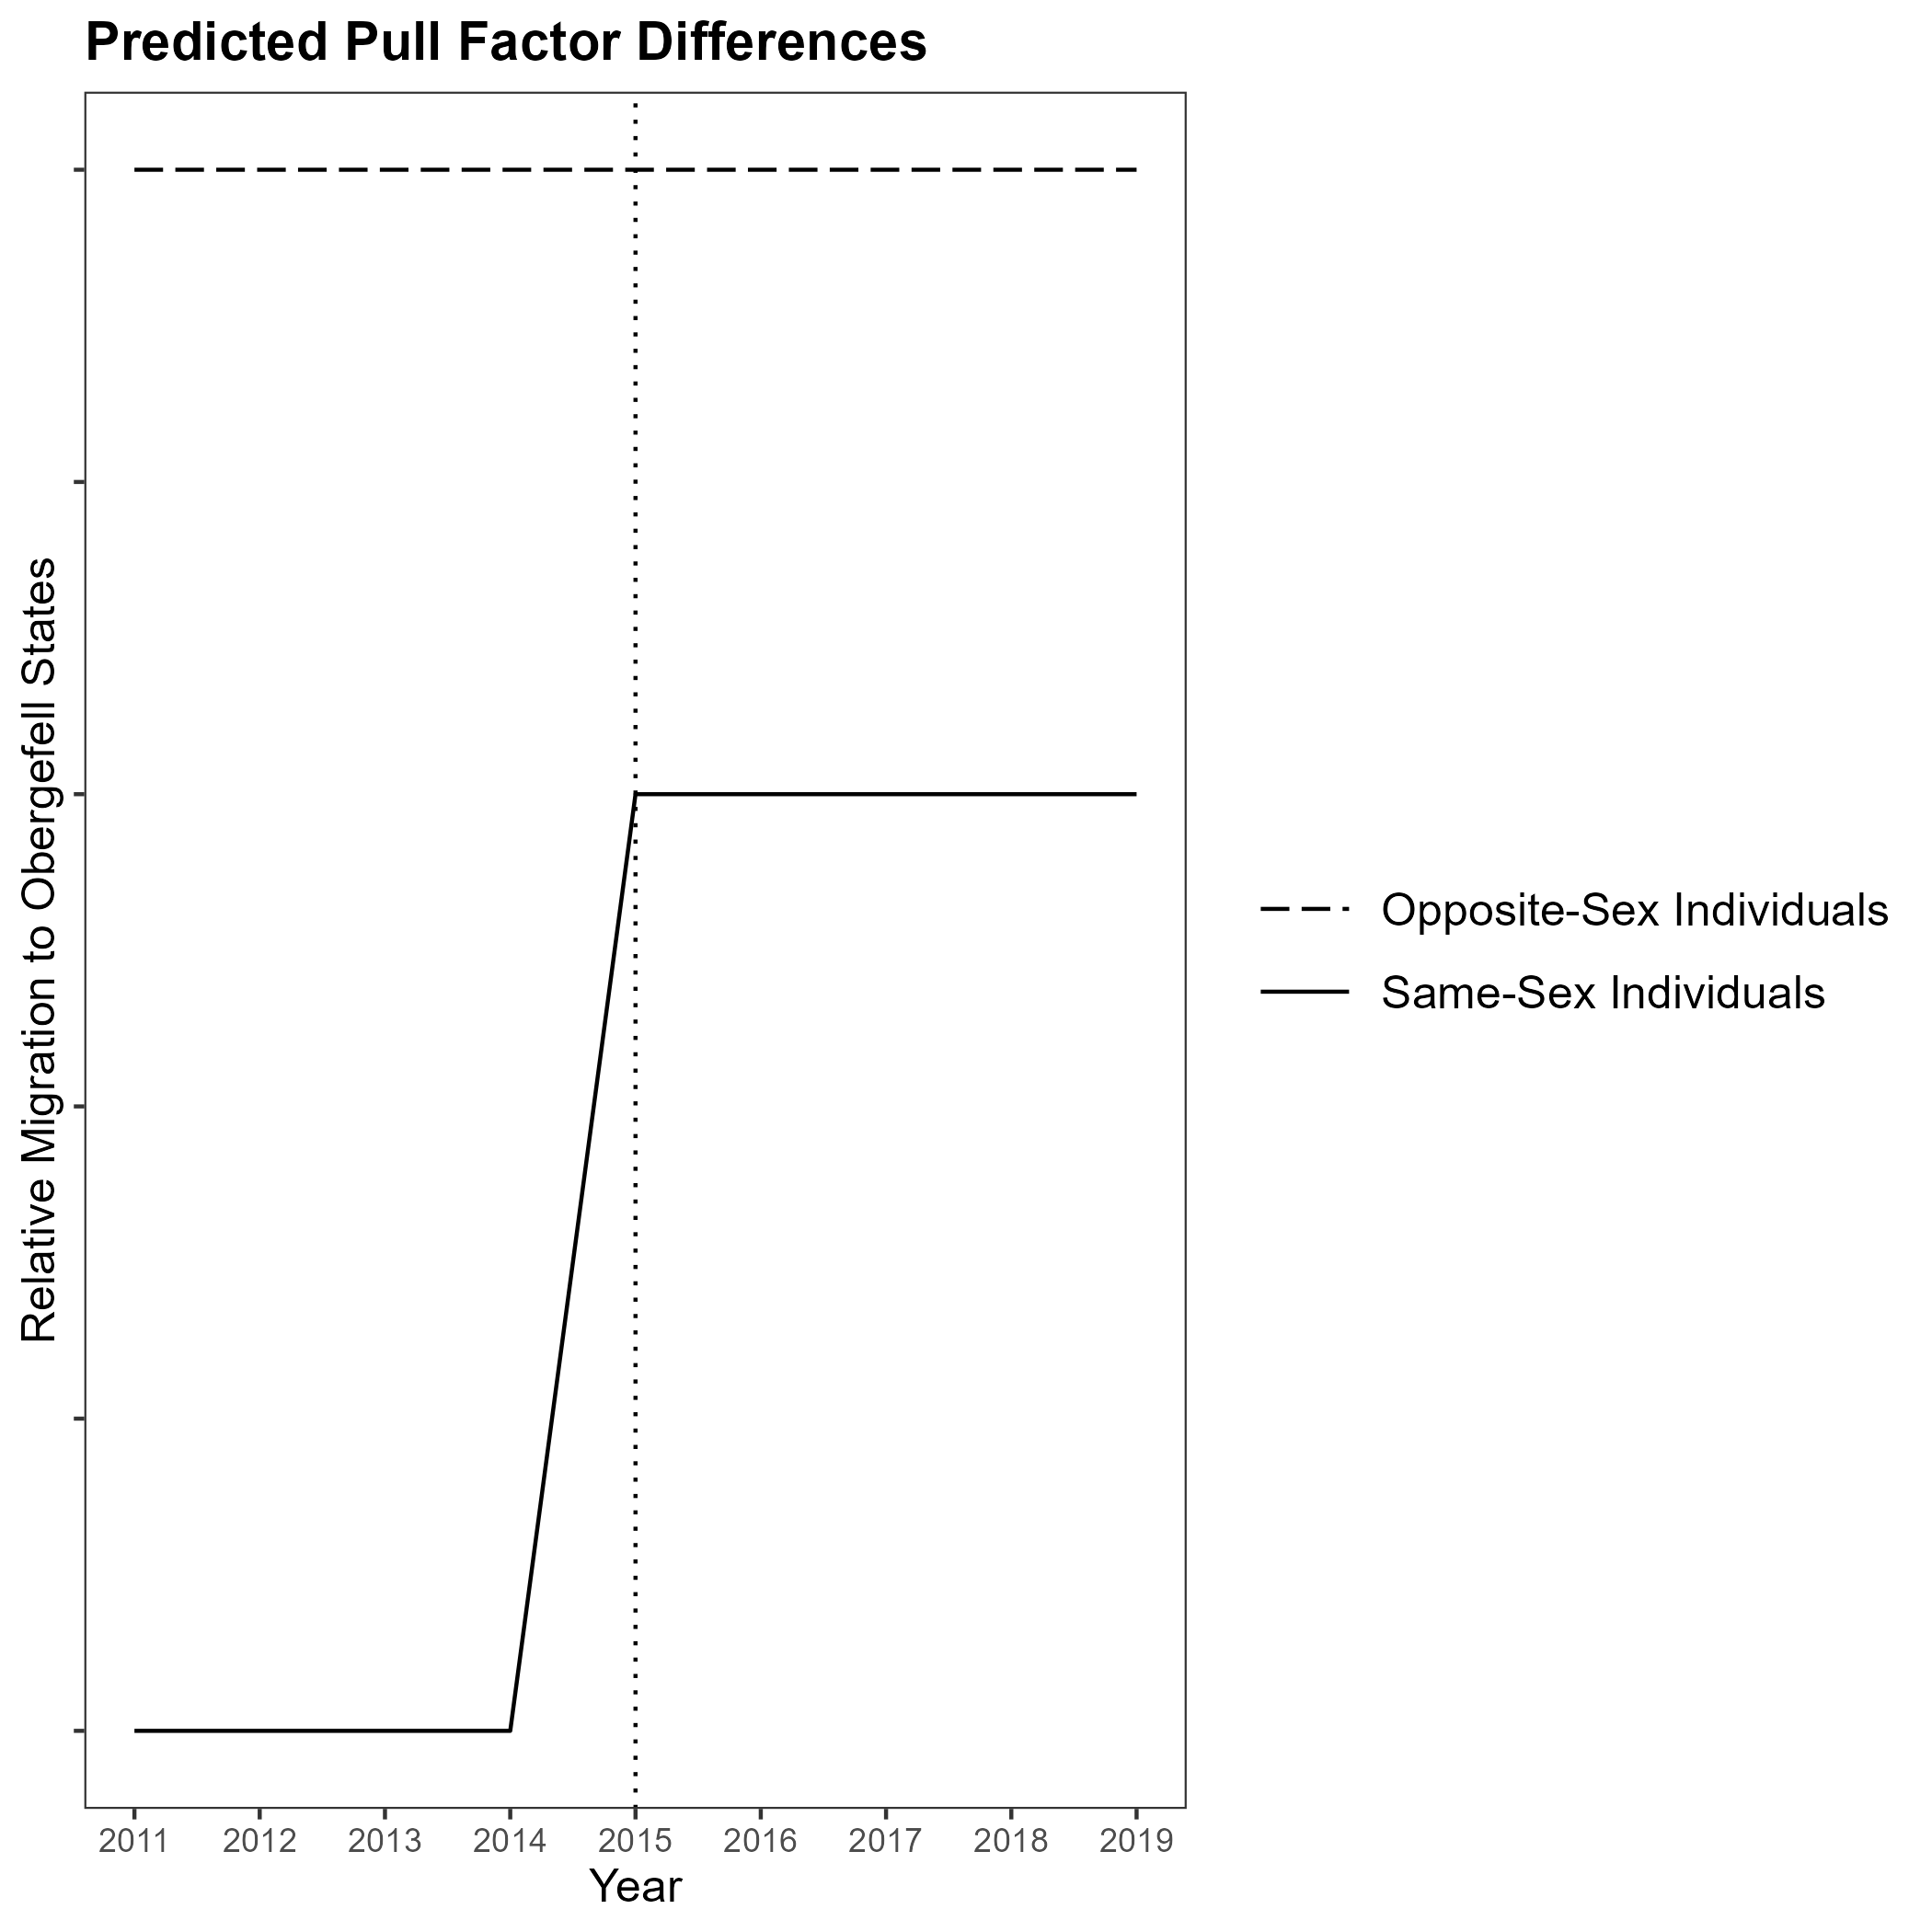
\includegraphics[width=0.75\linewidth]{outputs/summary_stats/ex_post_diffs.png}
    \centering
    \caption{}
    \label{fig: ex_post_diffs}
\end{figure}

\begin{figure}[htbp]
    \centering
    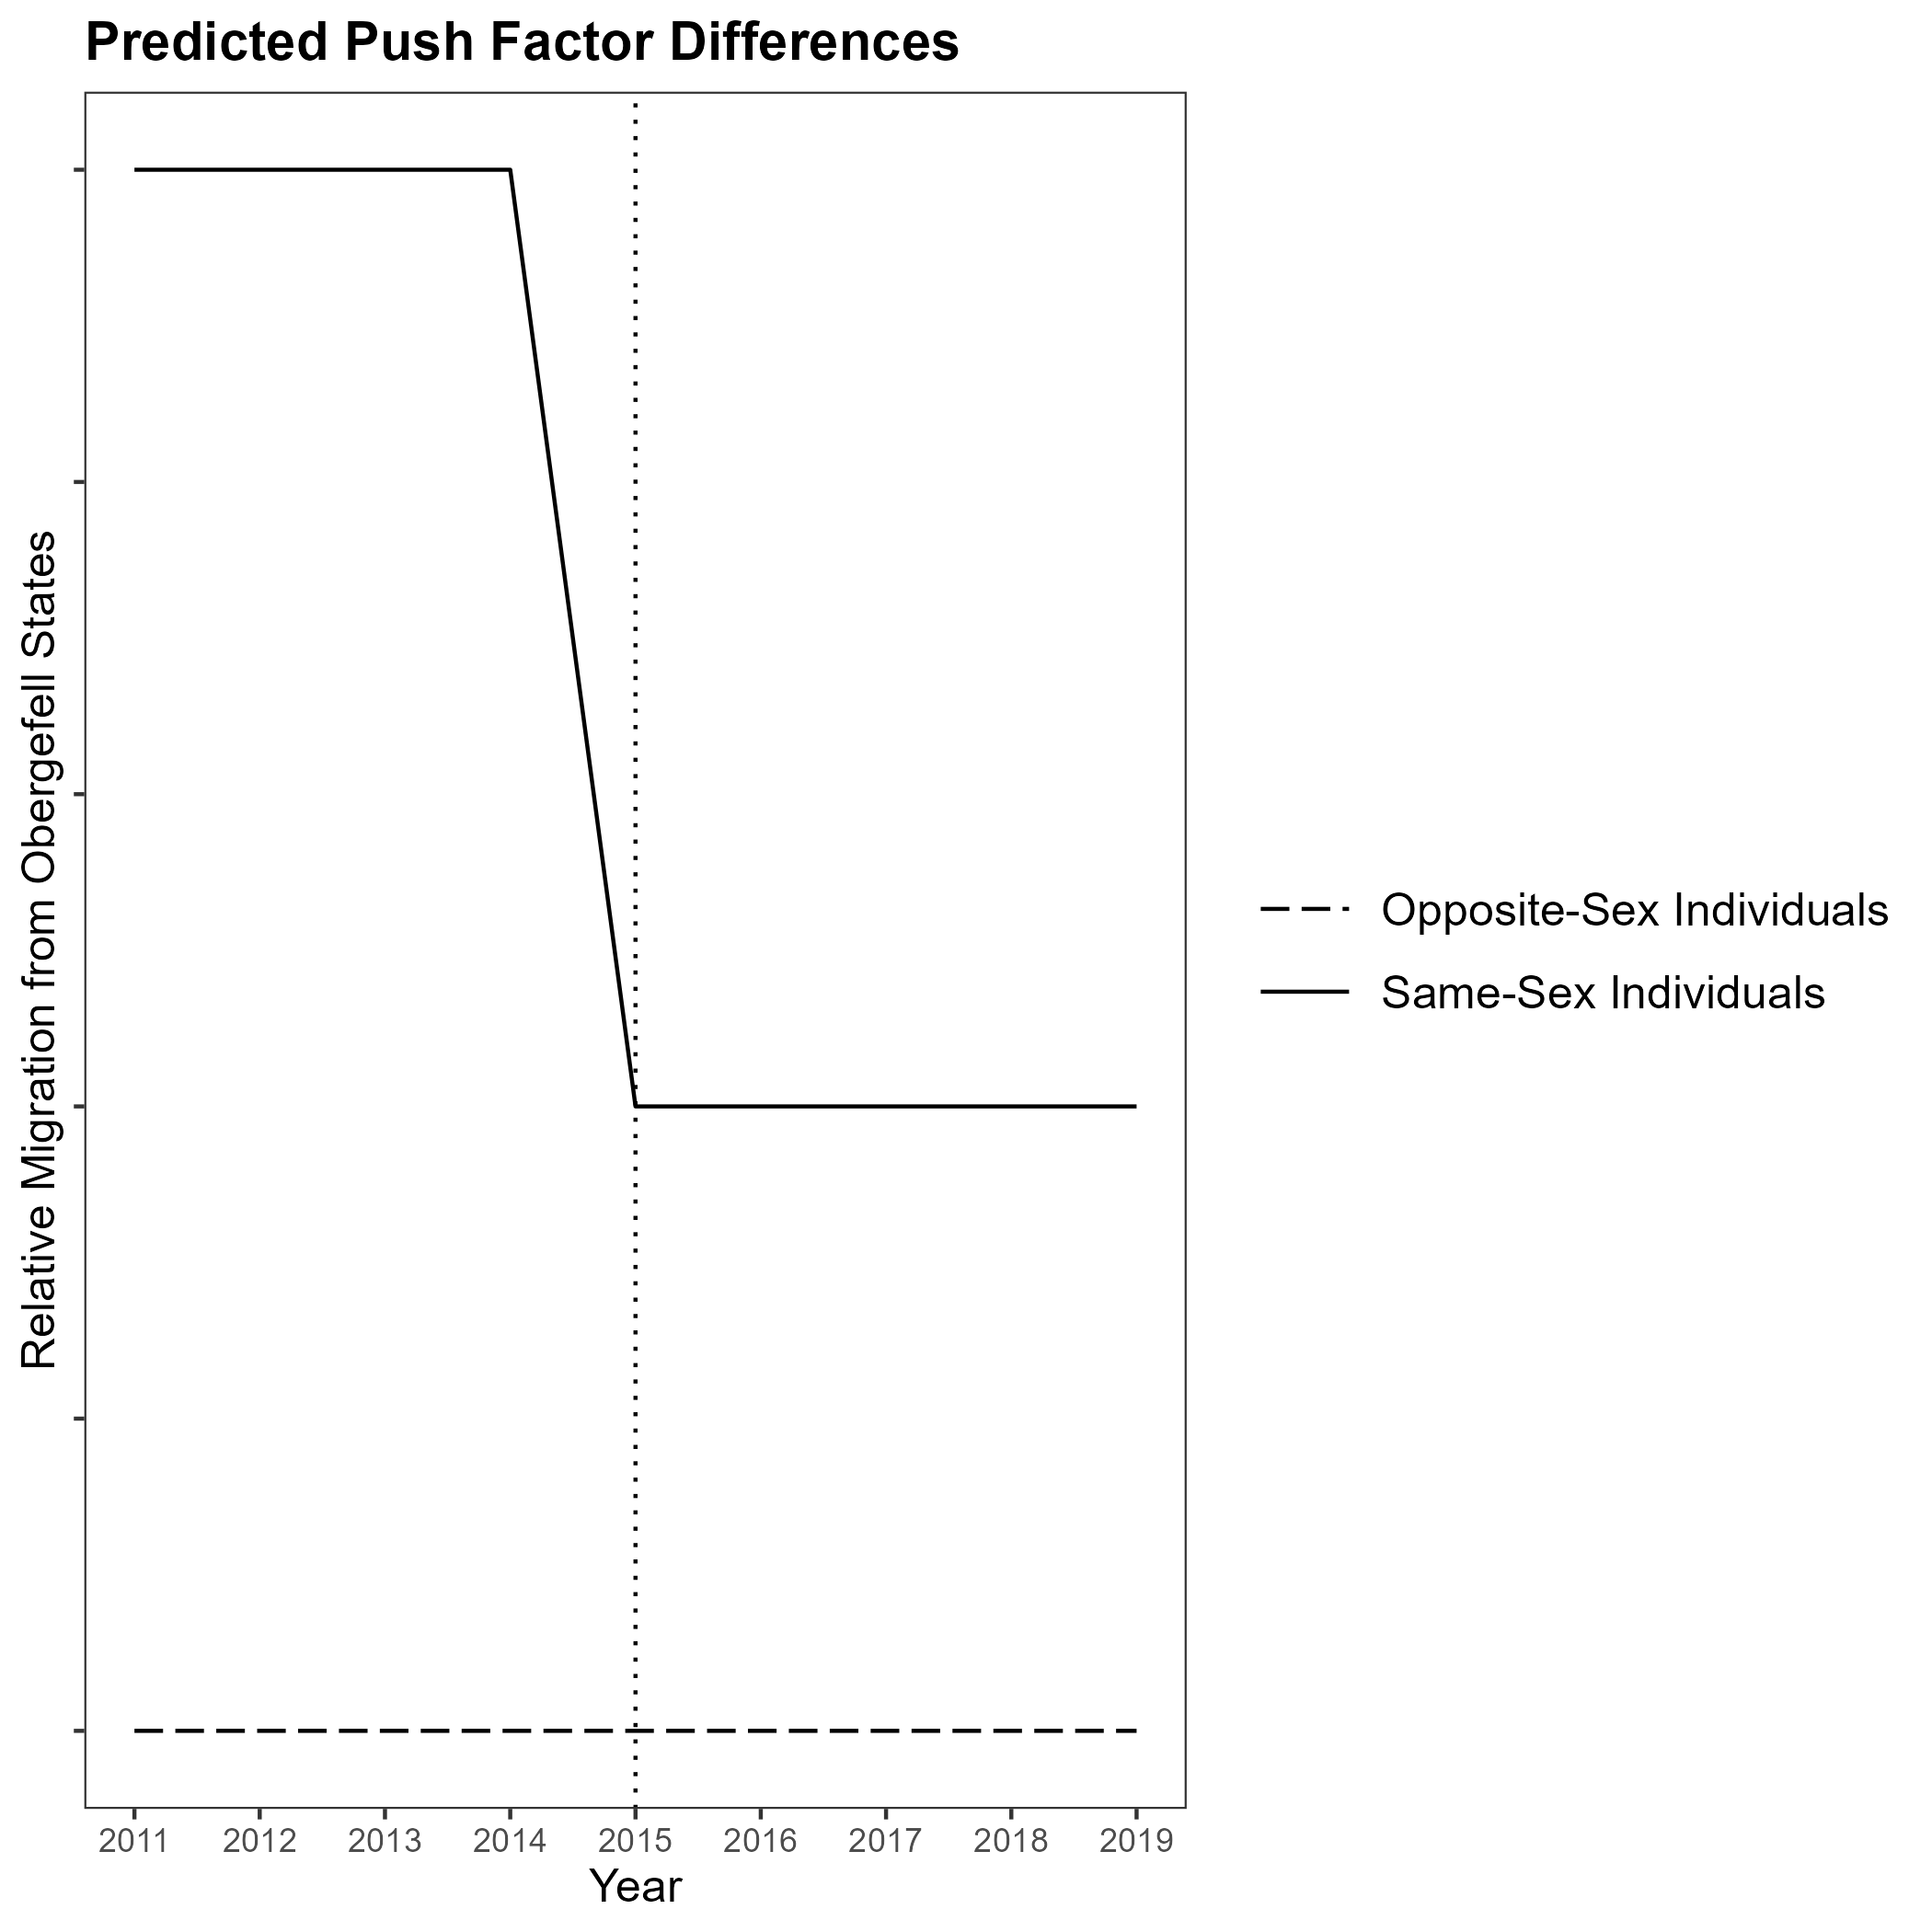
\includegraphics[width=0.75\linewidth]{outputs/summary_stats/ex_ante_diffs.png}
    \caption{}
    \label{fig: ex_ante_diffs}
\end{figure}


\FloatBarrier
\subsection{Main Model} %ok still need to fix centering
I present results from my main pull factor model in table \ref{tab: expost_model} and from my main push factor model in table \ref{tab: exante_model}. In both tables, Column 1 reports the regression coefficient from a model that includes fixed effects for state, year, relationship type, and their interactions. Column 2 reports the regression coefficient of a model with these fixed effects and controls for sex, race, education level, the presence of children in the household, income level, and age. Column 3 reports the regression coefficients of a model with additional controls for an individual’s birth state. I will primarily focus discussion on column 3 coefficients, as they incorporate the most comprehensive set of controls.

\begin{figure}[htbp]
    \centering
    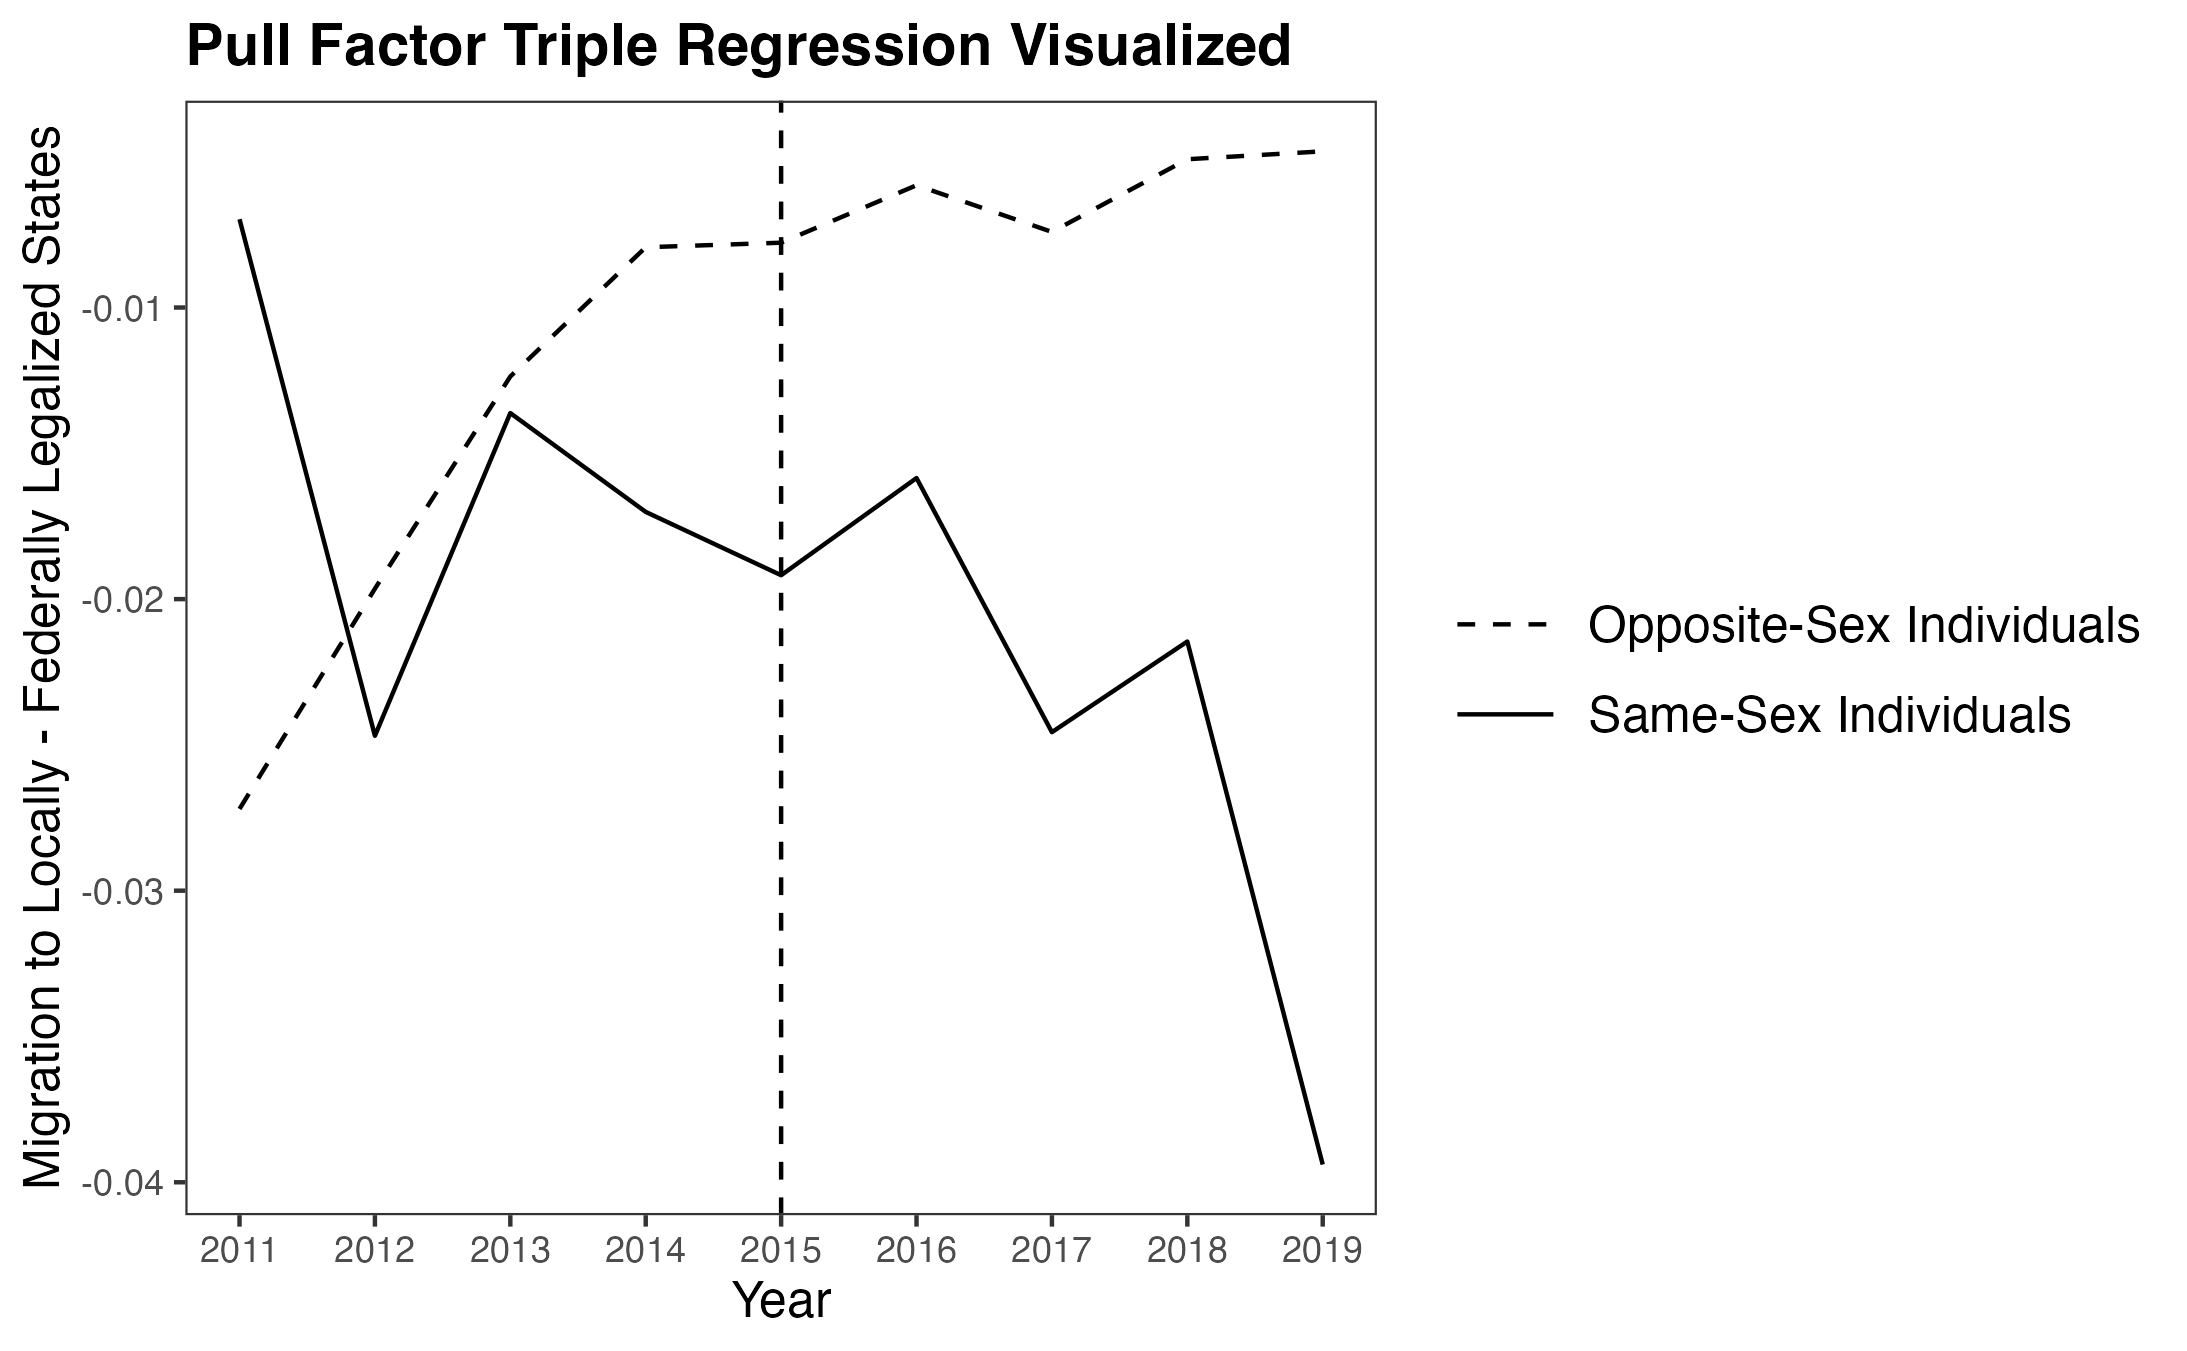
\includegraphics[width=0.75\linewidth]{outputs/summary_stats/post_diffs.png}
    \caption{}
    \label{fig: post_diffs}
\end{figure}

\begin{figure}[htbp]
    \centering
    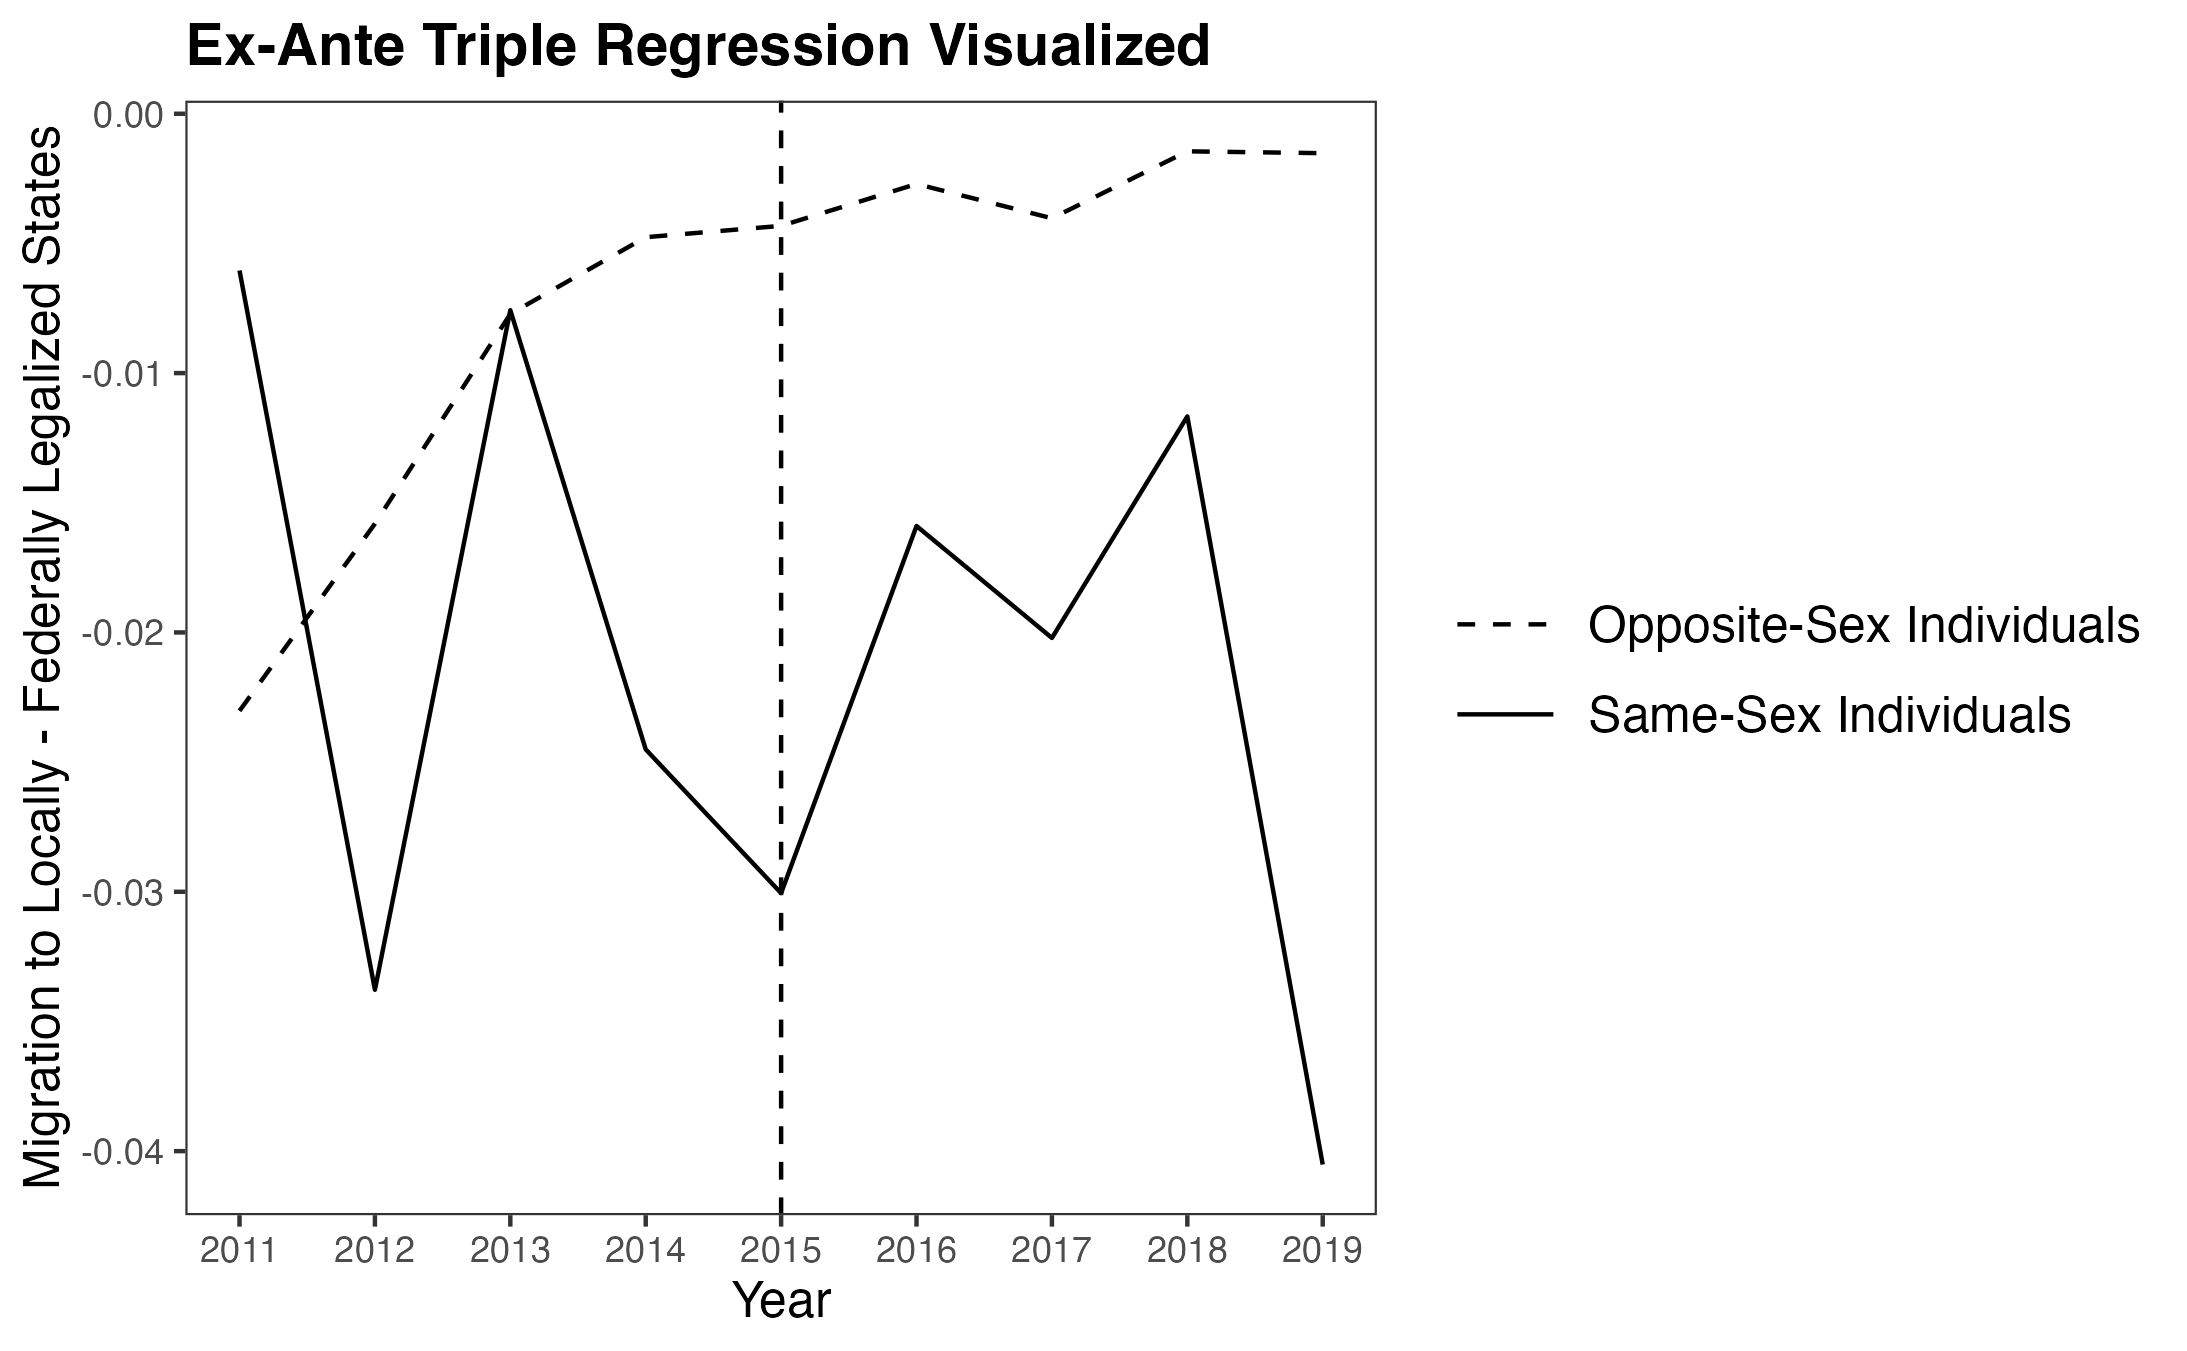
\includegraphics[width=0.75\linewidth]{outputs/summary_stats/ante_diffs.png}
    \caption{}
    \label{fig: ante_diffs}
\end{figure}

Before I discuss results, it is important to note that triple difference regressions assume parallel differences across groups. Figures \ref{fig: post_diffs} and \ref{fig: ante_diffs} show that this assumption is violated for these two main models. This might be related to how I define \textit{Obergefell}-legalized states: between 2011 and 2015, the composition of these states shifts as they rapidly adopt marriage equality at the state level. As a result, migration differences are influenced by varying definitions of \textit{Obergefell}-legalized states over time. This means that any results should be interpreted with caution.
%keep thinking about this 

\begin{table}[htbp]
    \centering
    \caption{Main Pull Factor Model}
    \label{tab: expost_model}
    \begin{tabular}{lccc}
\multicolumn{4}{c}{Ex-Post Model} \\ \hline
 & (1) & (2) & (3) \\
VARIABLES & migrant & migrant & migrant \\ \hline
 &  &  &  \\
1.in\_samesex\#1.expost\_old\_legal\#1.post\_2015 & -0.015* & -0.013* & 0.013 \\
 & (0.007) & (0.006) & (0.033) \\
Constant & 0.106*** & 0.394*** & 3.356*** \\
 & (0.001) & (0.008) & (0.080) \\
 &  &  &  \\
Observations & 956,236,912 & 956,236,912 & 956,236,912 \\
 R-squared & 0.004 & 0.070 & 0.921 \\ \hline
\multicolumn{4}{c}{ Robust standard errors in parentheses} \\
\multicolumn{4}{c}{ *** p$<$0.01, ** p$<$0.05, * p$<$0.1} \\
\multicolumn{4}{c}{ Model 1 includes interaction terms and fixed effects only.} \\
\multicolumn{4}{c}{ )} \\
\multicolumn{4}{c}{ )} \\
\multicolumn{4}{c}{ )} \\
\multicolumn{4}{c}{ )} \\
\end{tabular}

\end{table}
\begin{table}[htbp]
    \centering
    \caption{Main Push Factor Model}
    \label{tab: exante_model}
    \begin{tabular}{lccc}
\multicolumn{4}{c}{Ex-Ante Model} \\ \hline
 & (1) & (2) & (3) \\
VARIABLES & migrant & migrant & migrant \\ \hline
 &  &  &  \\
1.in\_samesex\#1.exante\_old\_legal\#1.post\_2015 & -0.016 & -0.014 & 0.014 \\
 & (0.009) & (0.008) & (0.030) \\
Constant & 0.106*** & 0.394*** & 3.757*** \\
 & (0.001) & (0.007) & (0.123) \\
 &  &  &  \\
Observations & 956,236,912 & 956,236,912 & 956,236,912 \\
 R-squared & 0.003 & 0.069 & 0.912 \\ \hline
\multicolumn{4}{c}{ Robust standard errors in parentheses} \\
\multicolumn{4}{c}{ *** p$<$0.01, ** p$<$0.05, * p$<$0.1} \\
\multicolumn{4}{c}{p{\textwidth}}{ Model 1 includes interaction terms and fixed effects only. \newline
Model 2 includes interaction terms, fixed effects, and controls for sex, race, education, age, and income. \newline
Model 3 includes interaction terms, fixed effects, and controls for sex, race, education, age, income, and birthstate. \newline
Models 1 and 2 use a weighted sample. Model 3 uses a weighted and collapsed sample.} \\
\multicolumn{4}{c}{ )} \\
\multicolumn{4}{c}{ )} \\
\multicolumn{4}{c}{ )} \\
\multicolumn{4}{c}{ )} \\
\end{tabular}

\end{table}

In the pull factor model, column 3 coefficients are positive and statistically insignificant. A 95 percent confidence interval includes the null result (although this is not the case for model 1). This suggests that there is some support that \textit{Obergefell v. Hodges} increased relative gay migration to states that had not previously legalized same-sex marriage. This would suggest that \textit{Obergefell} legalization shared some similarities with earlier, state-wide legalization. However, this evidence should be interpreted with caution because of the relatively large standard error and statistical insignificance. These attributes could be related more to the small fraction of individuals in same-sex relationships in my sample- at about one percent- then the relationship between \textit{Obergefell v. Hodges} and migration, but more caution is still warranted.

In the push factor model, model 3 coefficients are positive and statistically insignificant. A 95 percent confidence interval includes the null result. This suggests that there is some support that \textit{Obergefell v. Hodges} also increased relative gay migration from states that had not previously legalized same-sex marriage. This would suggest that \textit{Obergefell} legalization also shared some differences with earlier, state-wide legalization. Perhaps, while \textit{Obergefell} legalization made all states look more similar from the outside, underlying social or institutional differences, visible only within states, persisted. However, for similar reasons as above, this evidence should also be interpreted with more caution.
%watch repetition
%think about if it is ok to drop “last paragraph” here detailing heterogeneity checks

\FloatBarrier
\subsection{Sex Heterogeneity}
%hmmm how start this off
%this is really not eloquent
Research by \citet{1} and \cite{12} found that marriage legalization impacted migration patterns of gay men more than gay women. They suggest that this difference could be partially explained by the varying levels of discrimination faced by each group, as gay men may experience higher levels of discrimination.  If gay men face more discrimination than gay women, they might be more sensitive to changes in marriage equality.

\begin{table}[htbp]
    \centering
    \caption{Pull Factor Model: Men}
    \label{tab: male_expost_model}
    \begin{tabular}{lccc}
\hline
 & (1) & (2) & (3) \\
VARIABLES & Model 1 & Model 2 & Model 3 \\ \hline
 &  &  &  \\
$\hat{\beta_1}$ & 0.014 & 0.007 & 0.008 \\
 & (0.009) & (0.038) & (0.043) \\
Constant & 0.102*** & 3.971*** & 3.826*** \\
 & (0.000) & (0.125) & (0.102) \\
 &  &  &  \\
Observations & 17,816 & 17,816 & 17,816 \\
 R-squared & 0.004 & 0.912 & 0.917 \\ \hline
\multicolumn{4}{c}{ Robust standard errors in parentheses} \\
\multicolumn{4}{c}{ *** p$<$0.01, ** p$<$0.05, * p$<$0.1} \\
\multicolumn{4}{p{0.6\linewidth}}{\footnotesize Column 1 reports the regression coefficient of a model with state, year, and relationship-type fixed effects including corresponding interactions; column 2 reports the regression coefficient of a model with these fixed effects and controls for sex, race, education level, the presence of children in the household, income level, and age; and column 3 reports the regression coefficients of a model with these fixed effects, controls, and controls for an individual’s birth state.} \\
\end{tabular}

\end{table}
%fix formatting still- see Mac default/archive
\begin{table}[htbp]
    \centering
    \caption{Push Factor Model: Men}
    \label{tab: male_exante_model}
    \begin{tabular}{lccc}
\multicolumn{4}{c}{Ex-Ante Model: Male} \\ \hline
 & (1) & (2) & (3) \\
VARIABLES & Model 1 & Model 2 & Model 3: Male \\ \hline
 &  &  &  \\
ante\_treatment & -0.009 & -0.005 & -0.004 \\
 & (0.010) & (0.035) & (0.039) \\
Constant & 0.099*** & 4.002*** & 3.978*** \\
 & (0.000) & (0.089) & (0.100) \\
 &  &  &  \\
Observations & 17,816 & 17,816 & 17,816 \\
 R-squared & 0.004 & 0.908 & 0.909 \\ \hline
\multicolumn{4}{c}{ Robust standard errors in parentheses} \\
\multicolumn{4}{c}{ *** p$<$0.01, ** p$<$0.05, * p$<$0.1} \\
\multicolumn{4}{c}{ See below.} \\
\end{tabular}

\end{table}
%\FloatBarrier
Here, I run the same regressions as above, but only look at men. Tables \ref{tab: male_expost_model} and \ref{tab: male_exante_model} report regression results for the pull factor and push factor models respectively. Results for a women-only specification can be found in the appendix (Tables \ref{tab: female_expost_model} and \ref{tab: female_exante_model}).
%\FloatBarrier
\begin{figure}[htbp]
    \centering
    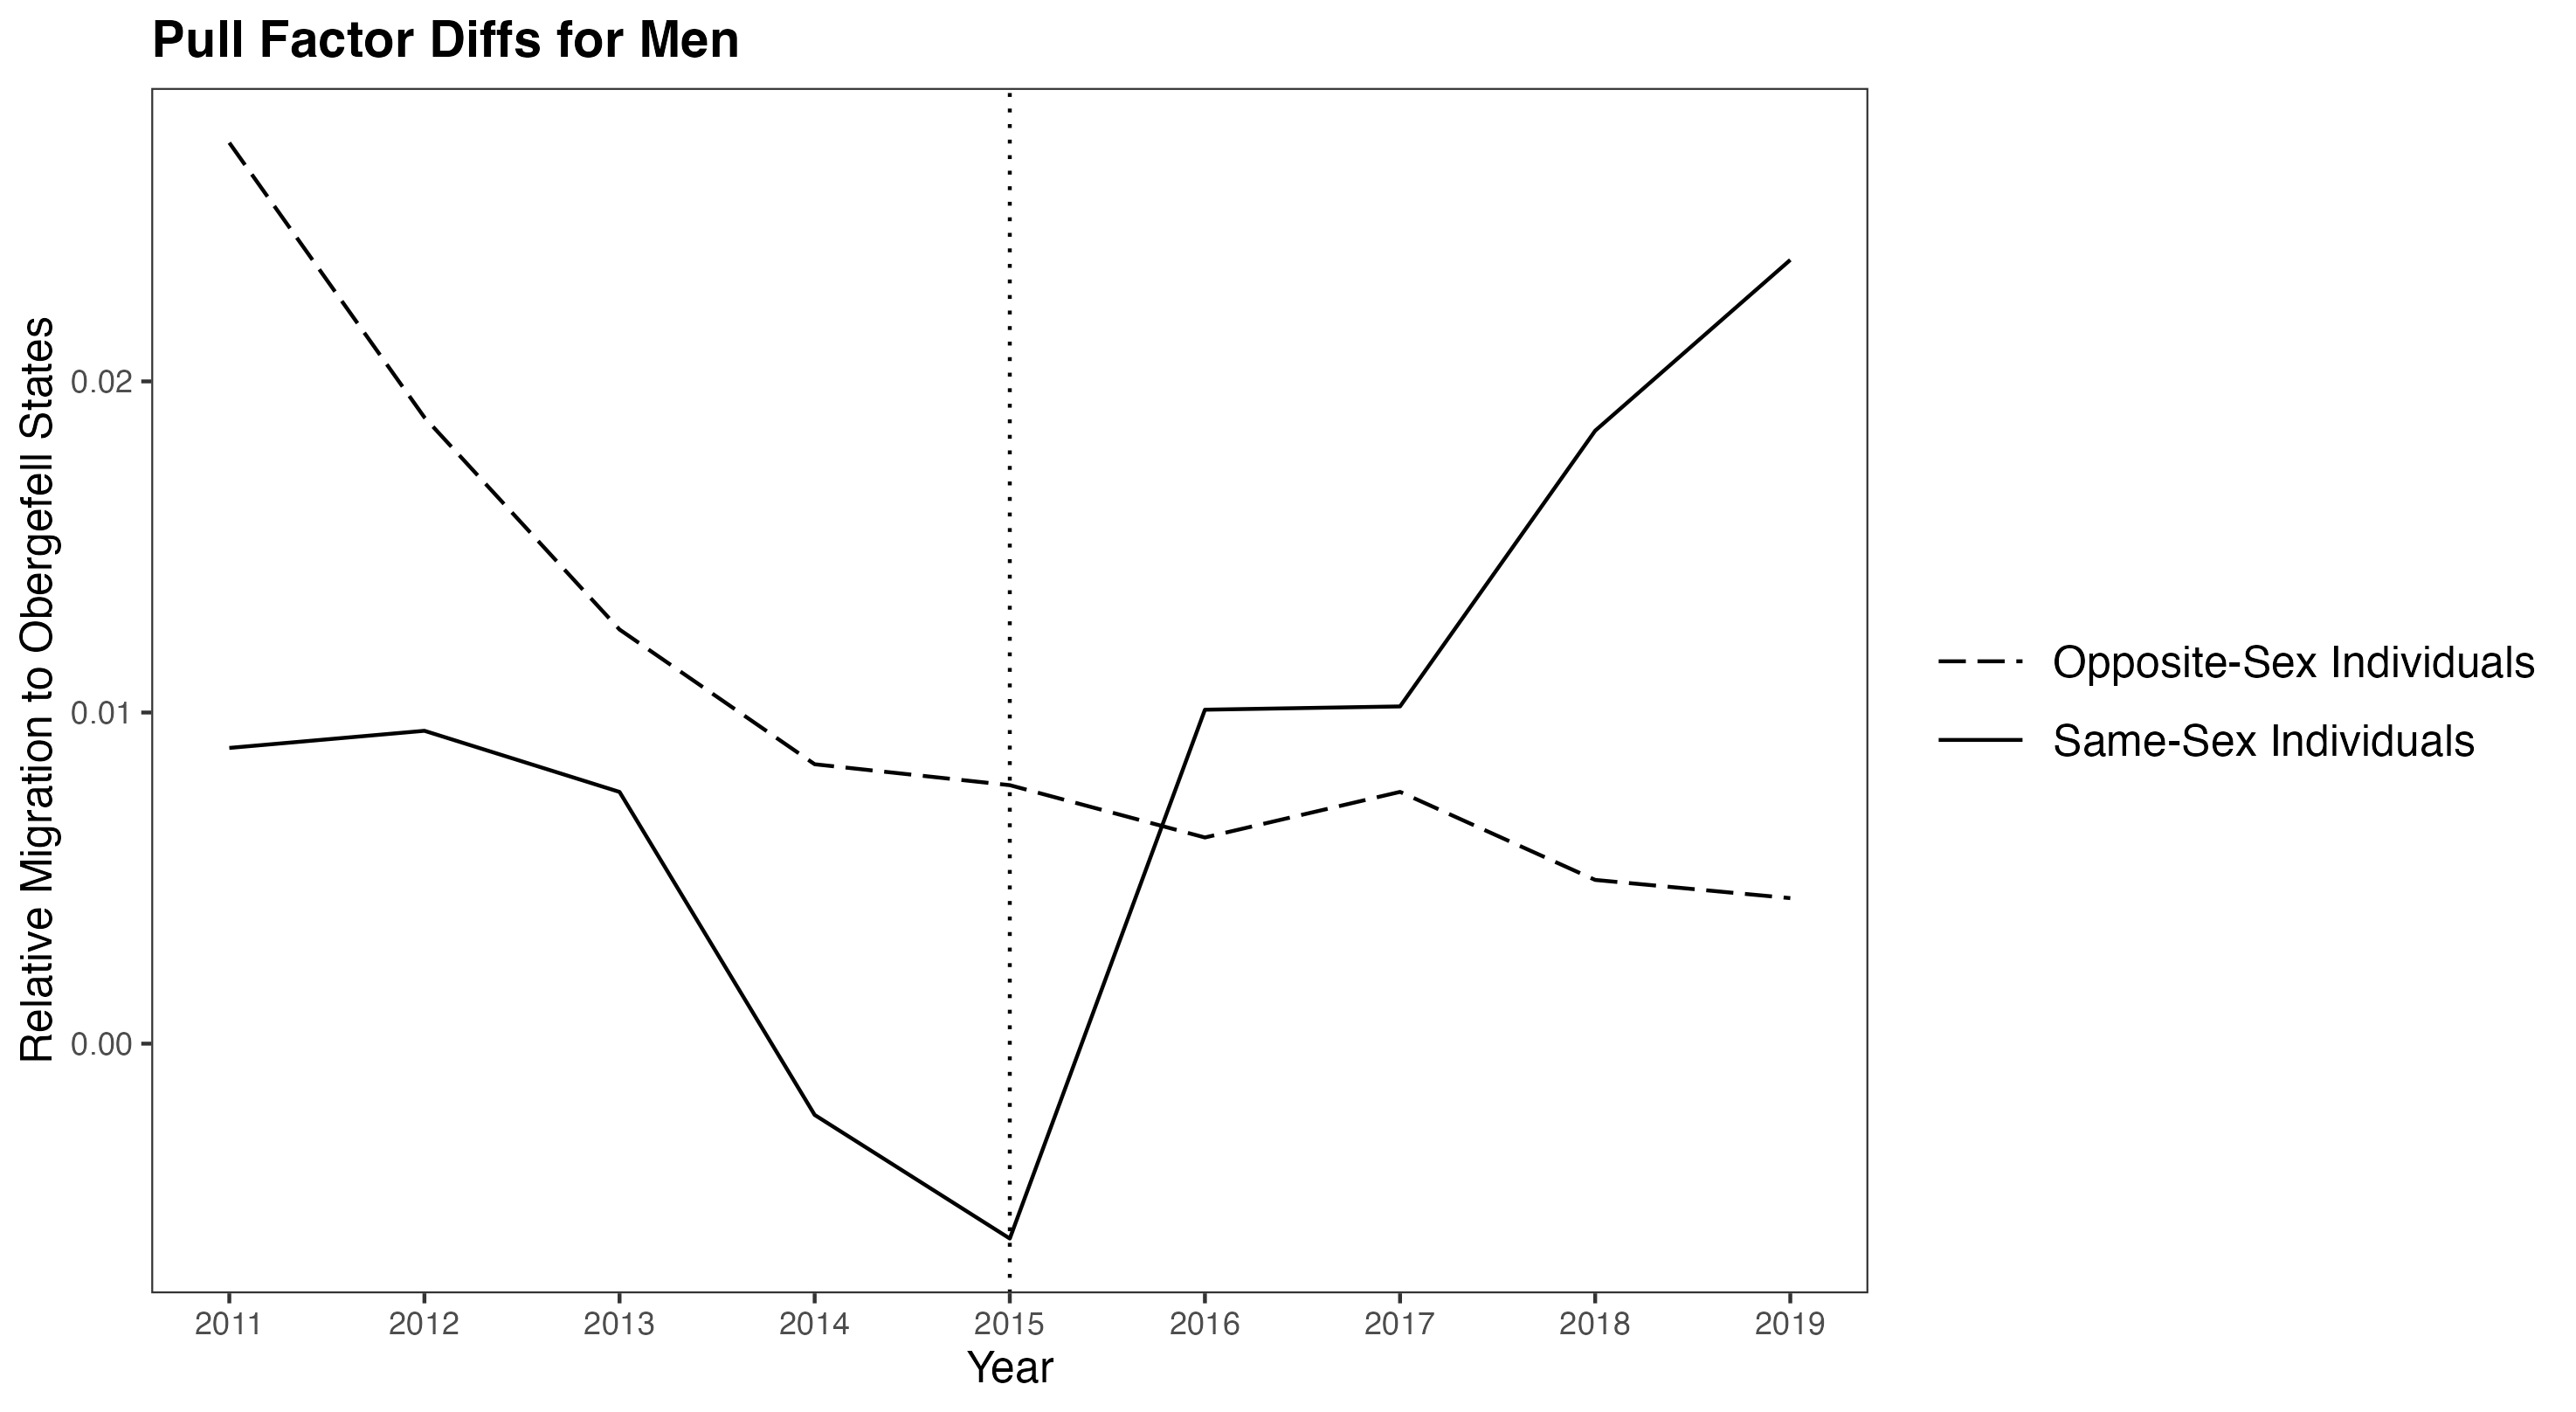
\includegraphics[width=1\linewidth]{outputs/summary_stats/men_post_diffs.png}
    \caption{}
    \label{fig: men_post_diffs}
\end{figure}
\begin{figure}[htbp]
    \centering
    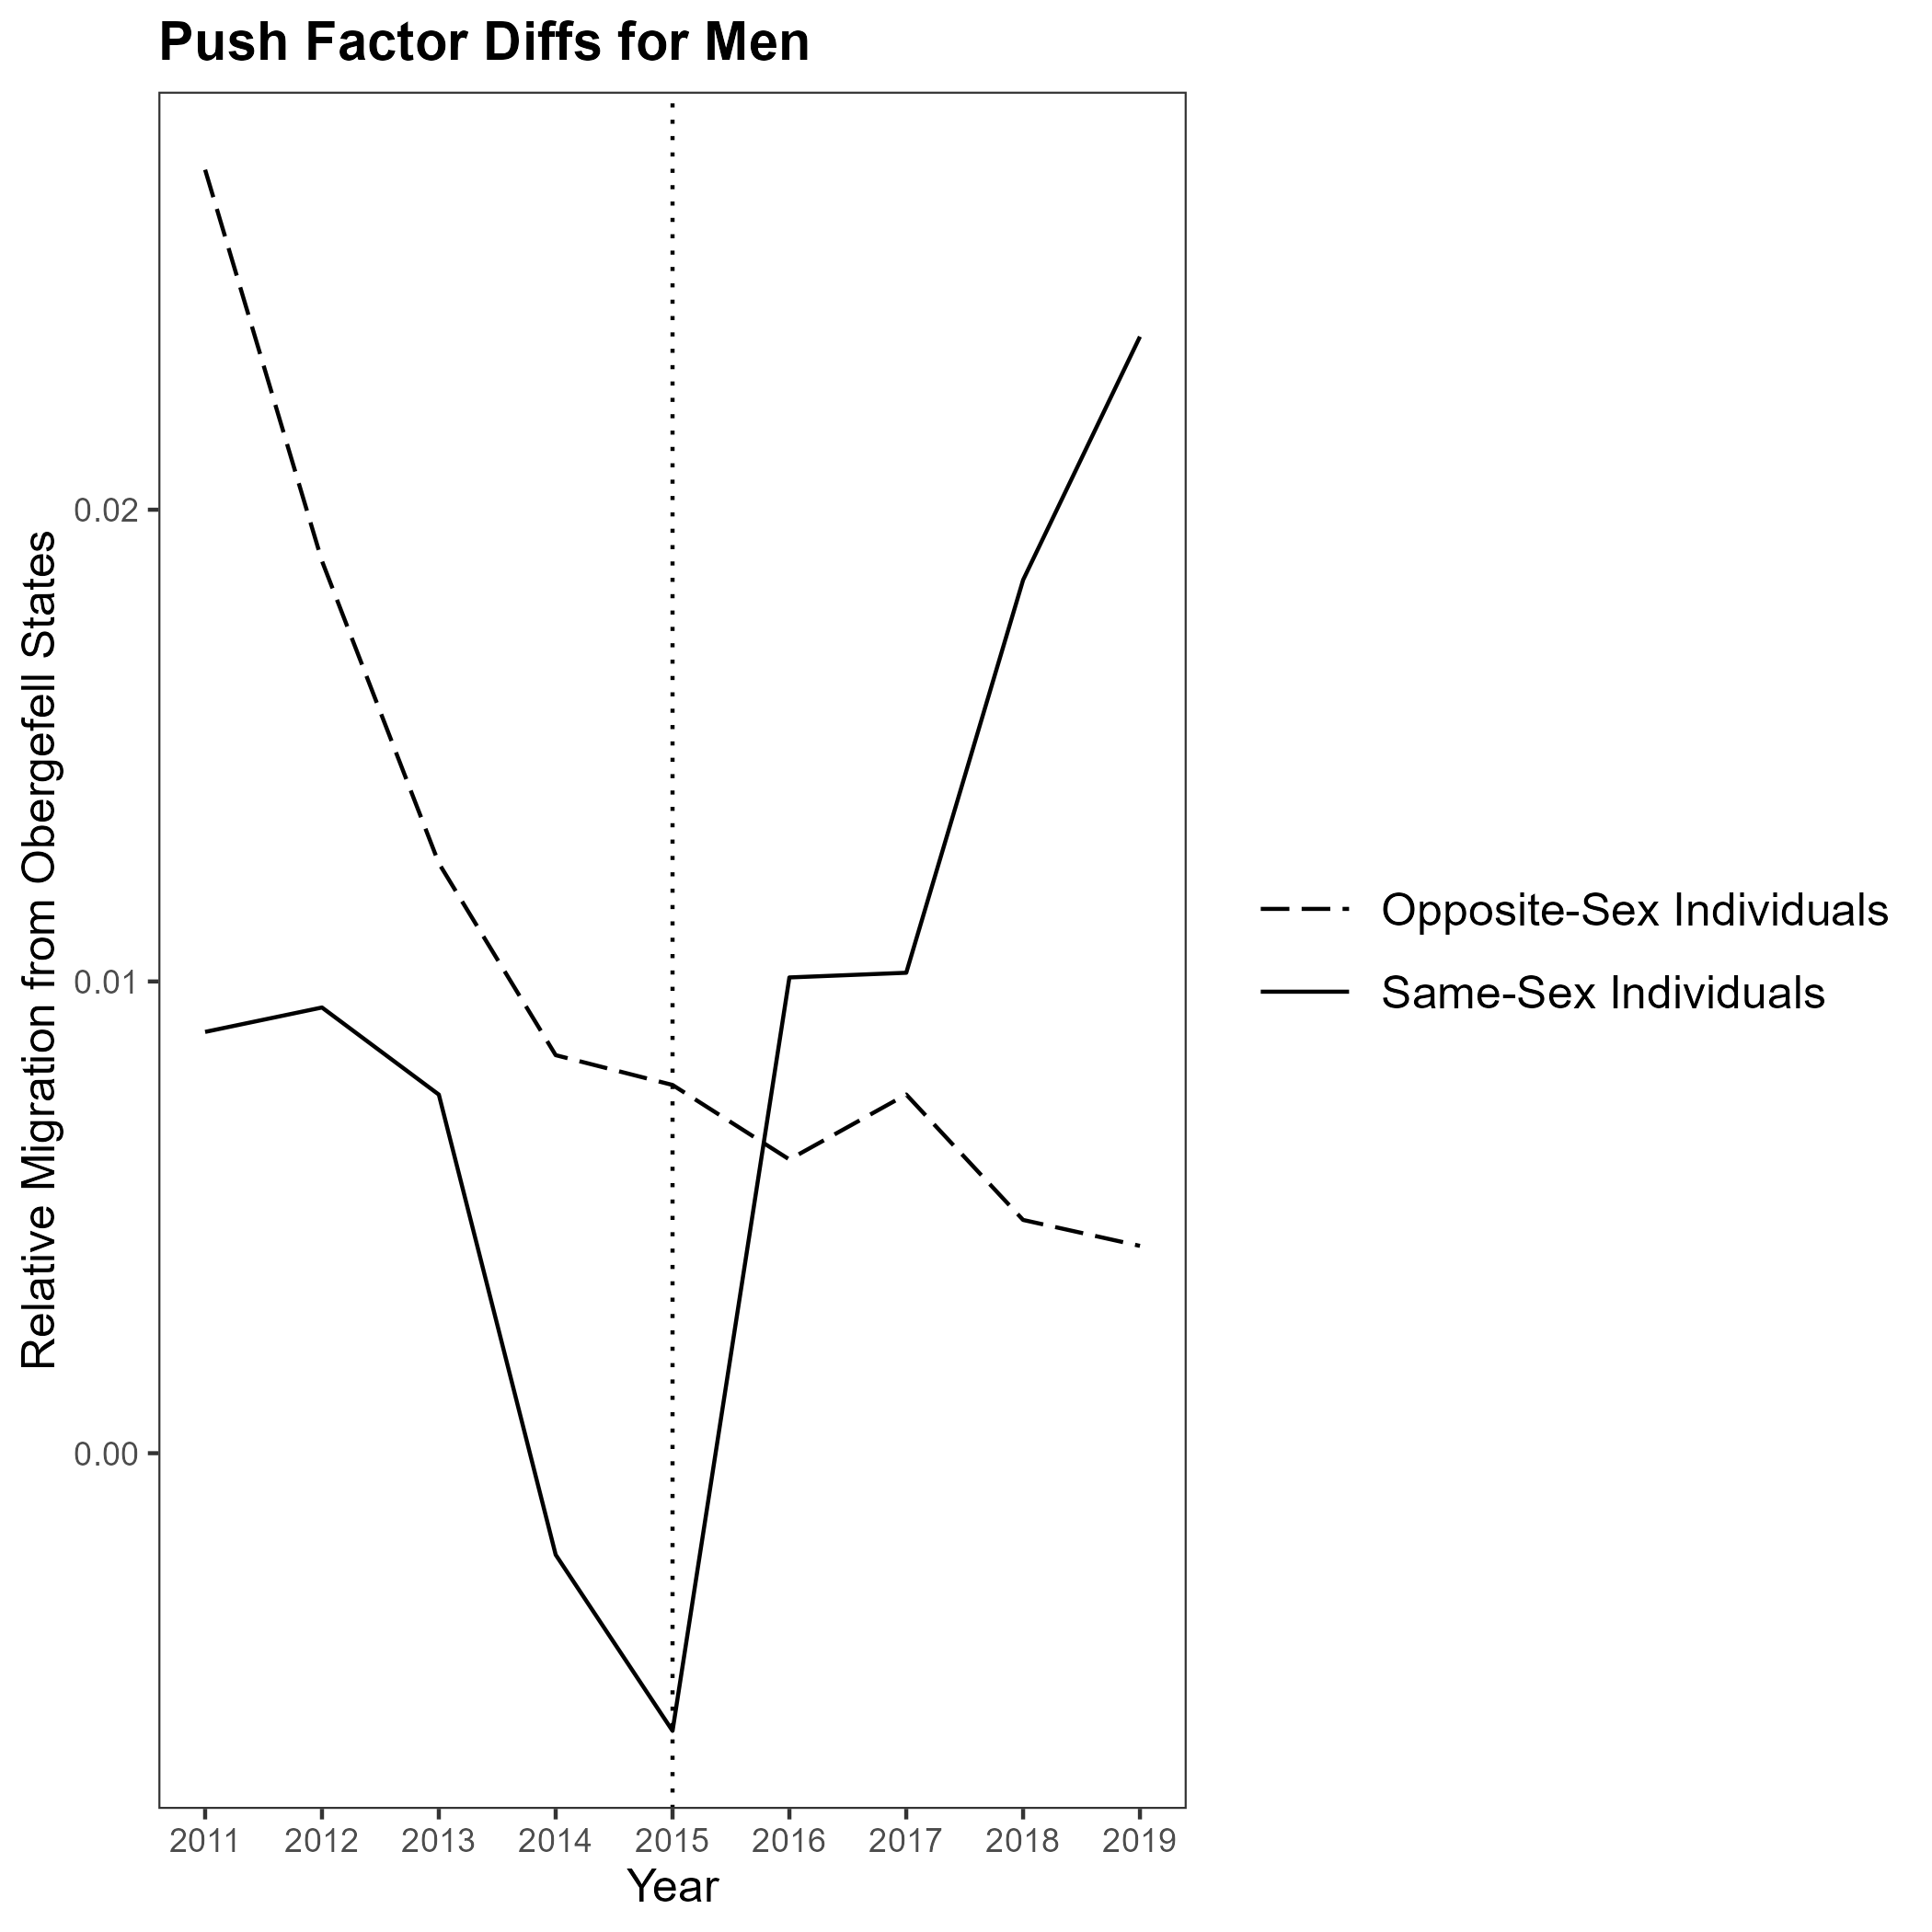
\includegraphics[width=1\linewidth]{outputs/summary_stats/men_ante_diffs.png}
    \caption{}
    \label{fig: men_ante_diffs}
\end{figure}

%separate out by gender to be clearer
%need more comment on parallel trends here
%comment on model 1?
%watch say gay men/men in same-sex relationships
As can be seen in figures \ref{fig: men_post_diffs} and \ref{fig: men_ante_diffs}, parallel trends seem to hold for the men-only sample (figures for the women-only sample can be found in the appendix). This suggests compositional variation obscured trends in the main model, and less caution should be taken in utilizing a triple difference model to understand the relationship between gay men and marriage equality. This confirms results from \citet{1} and \citet{12}. However, similar to the main model, both push and pull factor column 3 coefficients are positive, statistically insignificant, and have 95 percent confidence intervals that include the null result (again, similarly, the pull factor column 1 coefficient has a smaller confidence interval). The larger coefficient magnitudes in the men-only sample compared to the main model suggest that the observed effects in the full sample are primarily driven by men in same-sex relationships. For men in same-sex relationships, there is some evidence that \textit{Obergefell}-legalization increased migration to states relative to those that legalized earlier, but decreased migration out of those states.

\FloatBarrier
\subsection{Region Heterogeneity}

%state which way bias could go?
\textit{Obergefell v. Hodges} only introduced marriage equality to states in the south and midwest, as defined by the Census. Approximately 50 percent of my sample lived in these regions, with individuals in same-sex relationships representing a notably smaller proportion compared to those in different-sex relationships (table \ref{region_1})\footnote{Table \ref{region_2} in the appendix includes statistics on the west and northeast.}. Many inter-state migrants travel across regions. However, as \citet{1} notes, distance likely affects migration decisions. Individuals further from \textit{Obergefell}-legalized states might be less sensitive to the effect of \textit{Obergefell v. Hodges} than individuals closer. Accounting for an individual’s region might help proxy the effect of distance.
\begin{table}[htbp]

\caption{Summary Statistics by Region (1)}
\label{region_1} %added
\centering
\begin{tabular}[t]{rrrrr}
\toprule
\multicolumn{1}{c}{ } & \multicolumn{2}{c}{\% in the Midwest} & \multicolumn{2}{c}{\% in the South} \\
\cmidrule(l{3pt}r{3pt}){2-3} \cmidrule(l{3pt}r{3pt}){4-5}
Year & Same-Sex & Different-Sex & Same-Sex & Different-Sex\\
\midrule
2011 & 20 & 25 & 33 & 38\\
2012 & 20 & 25 & 34 & 38\\
2013 & 19 & 25 & 34 & 38\\
2014 & 20 & 25 & 35 & 39\\
2015 & 19 & 25 & 35 & 38\\
2016 & 19 & 25 & 36 & 38\\
2017 & 19 & 25 & 36 & 38\\
2018 & 19 & 25 & 36 & 38\\
2019 & 18 & 24 & 37 & 38\\
\bottomrule
\end{tabular}
\vspace{0.5em}
\begin{minipage}{0.85\textwidth} % Adjust width as needed
\small \textbf{Note:} The Midwest includes Illinois, Indiana, Michigan, Ohio, Wisconsin, Iowa, Kansas, Minnesota, Missouri, Nebraska, North Dakota, and South Dakota. The South includes Delaware, District of Columbia, Florida, Georgia, Maryland, North Carolina, South Carolina, Virginia, West Virginia, Alabama, Kentucky, Mississippi, Tennessee, Arkansas, Louisiana, Oklahoma/Indian Territory, and Texas. These definitions are set by the ACS.
\end{minipage}
\end{table}


%oi how to report tables without clogging everything up
I do this by running the main pull factor regression on a sample of individuals in the south and midwest, respectively, and running the main push factor regression on a sample of individuals coming from the south and midwest, respectively. Tables \ref{tab: south_expost_model} and \ref{tab: south_exante_model} report results for the southern models and tables \ref{tab: midwest_expost_model} and \ref{tab: midwest_exante_model} report results for the midwestern models. Tables for the west and northeast can be found in the appendix (These include tables \ref{tab: west_expost_model}, \ref{tab: west_exante_model}, \ref{tab: northeast_expost_model}, and \ref{tab: northeast_exante_model}.).


\begin{figure}[htbp]
    \centering
    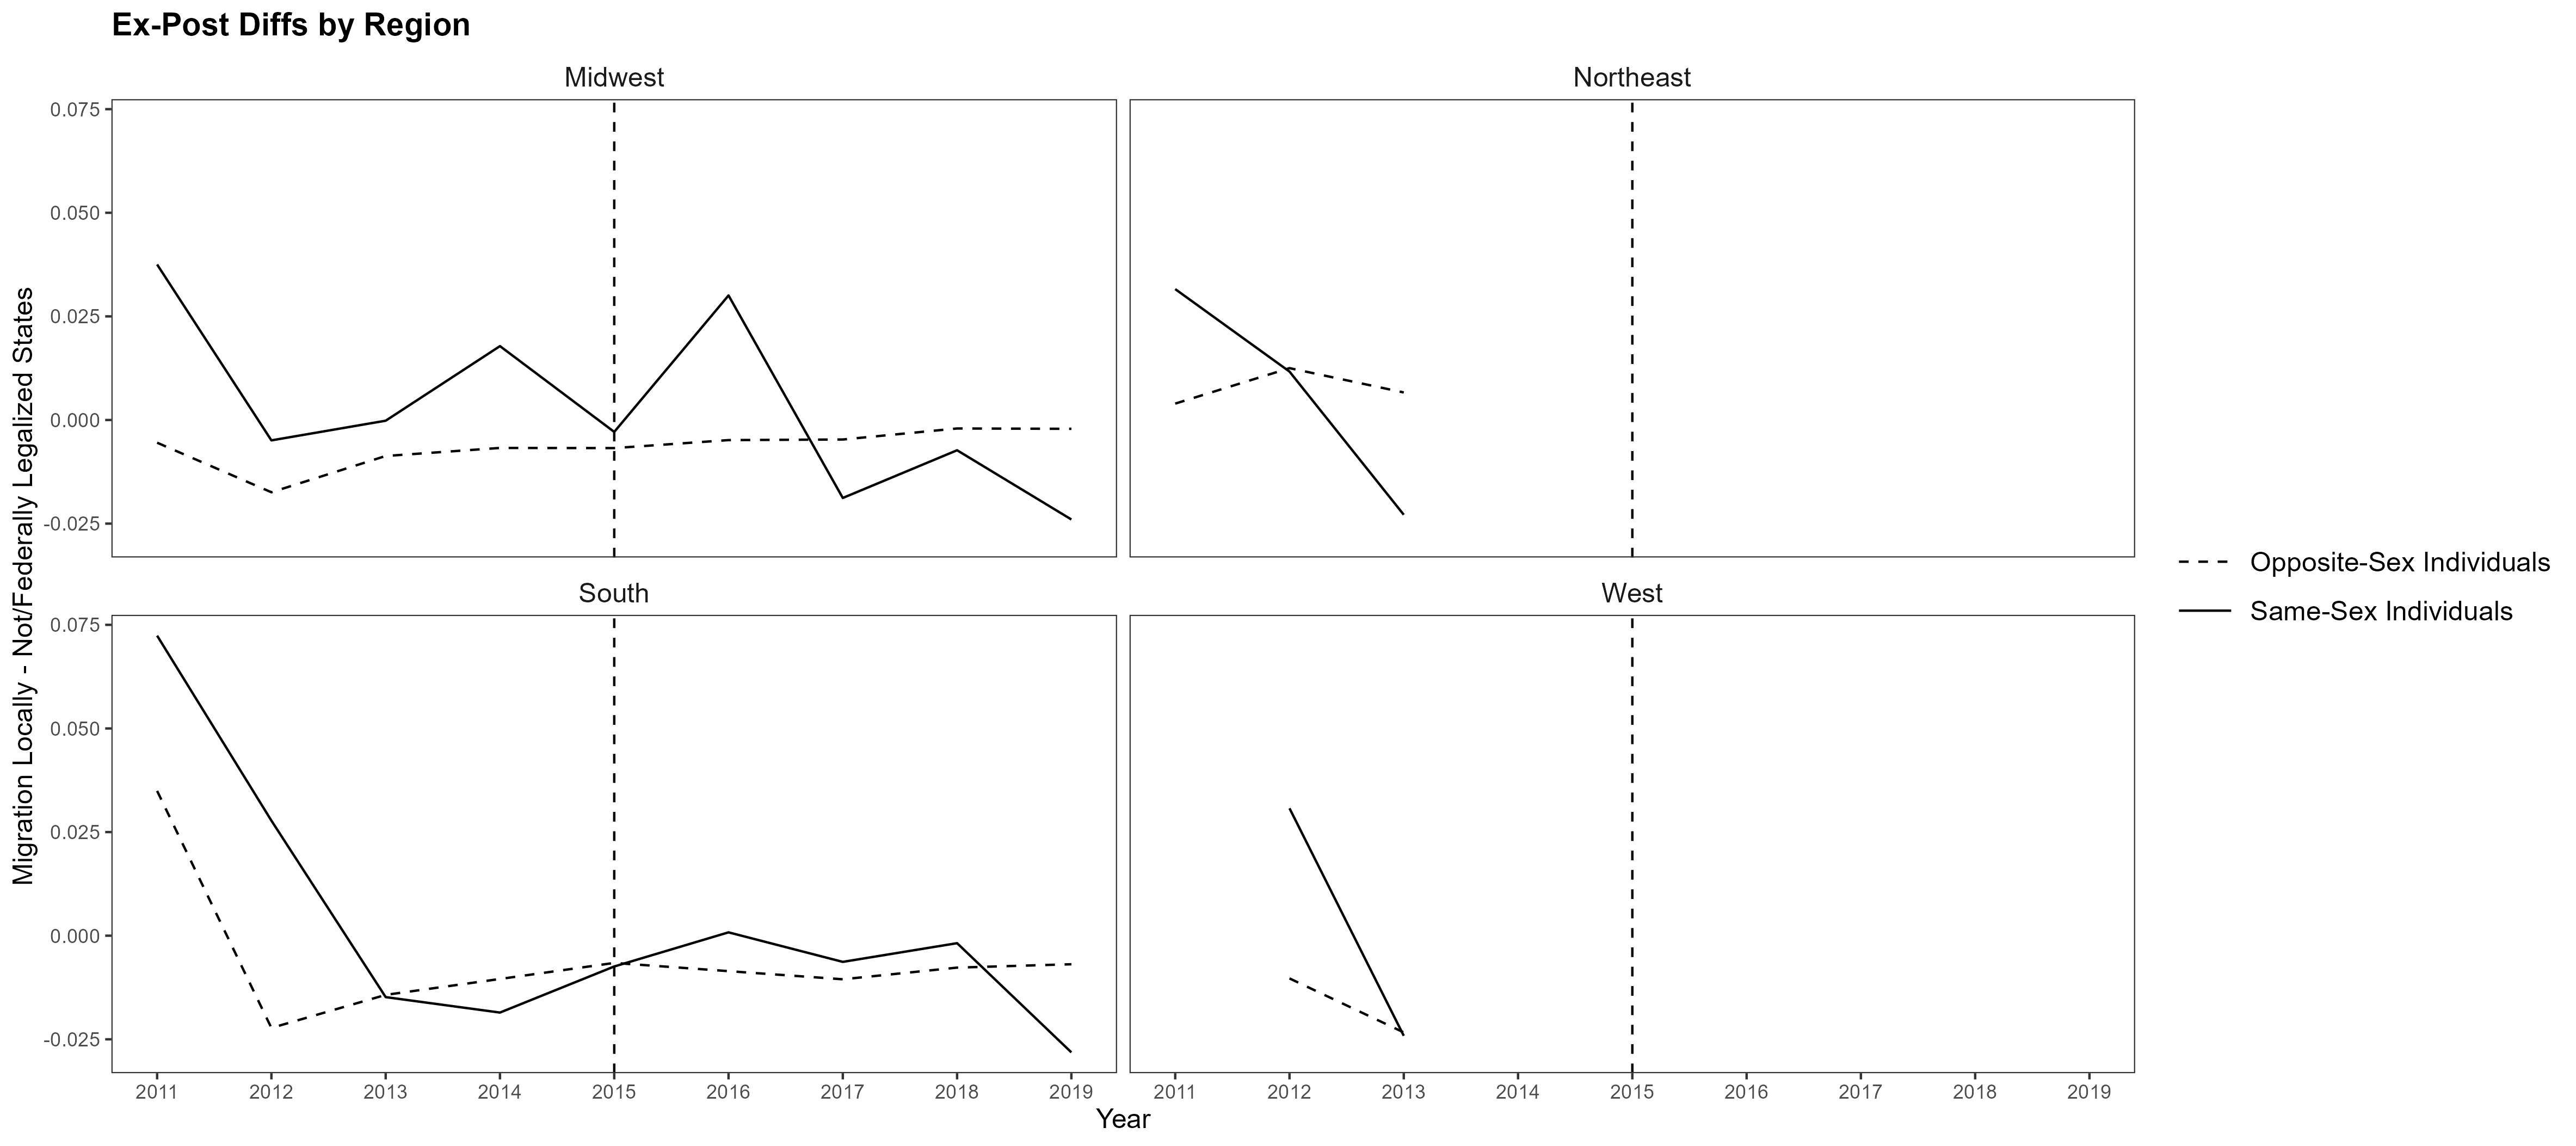
\includegraphics[width=1\linewidth]{outputs/summary_stats/region_post_diffs.png}
    \caption{}
    \label{fig: region_post_diffs}
\end{figure}

\begin{figure}[htbp]
    \centering
    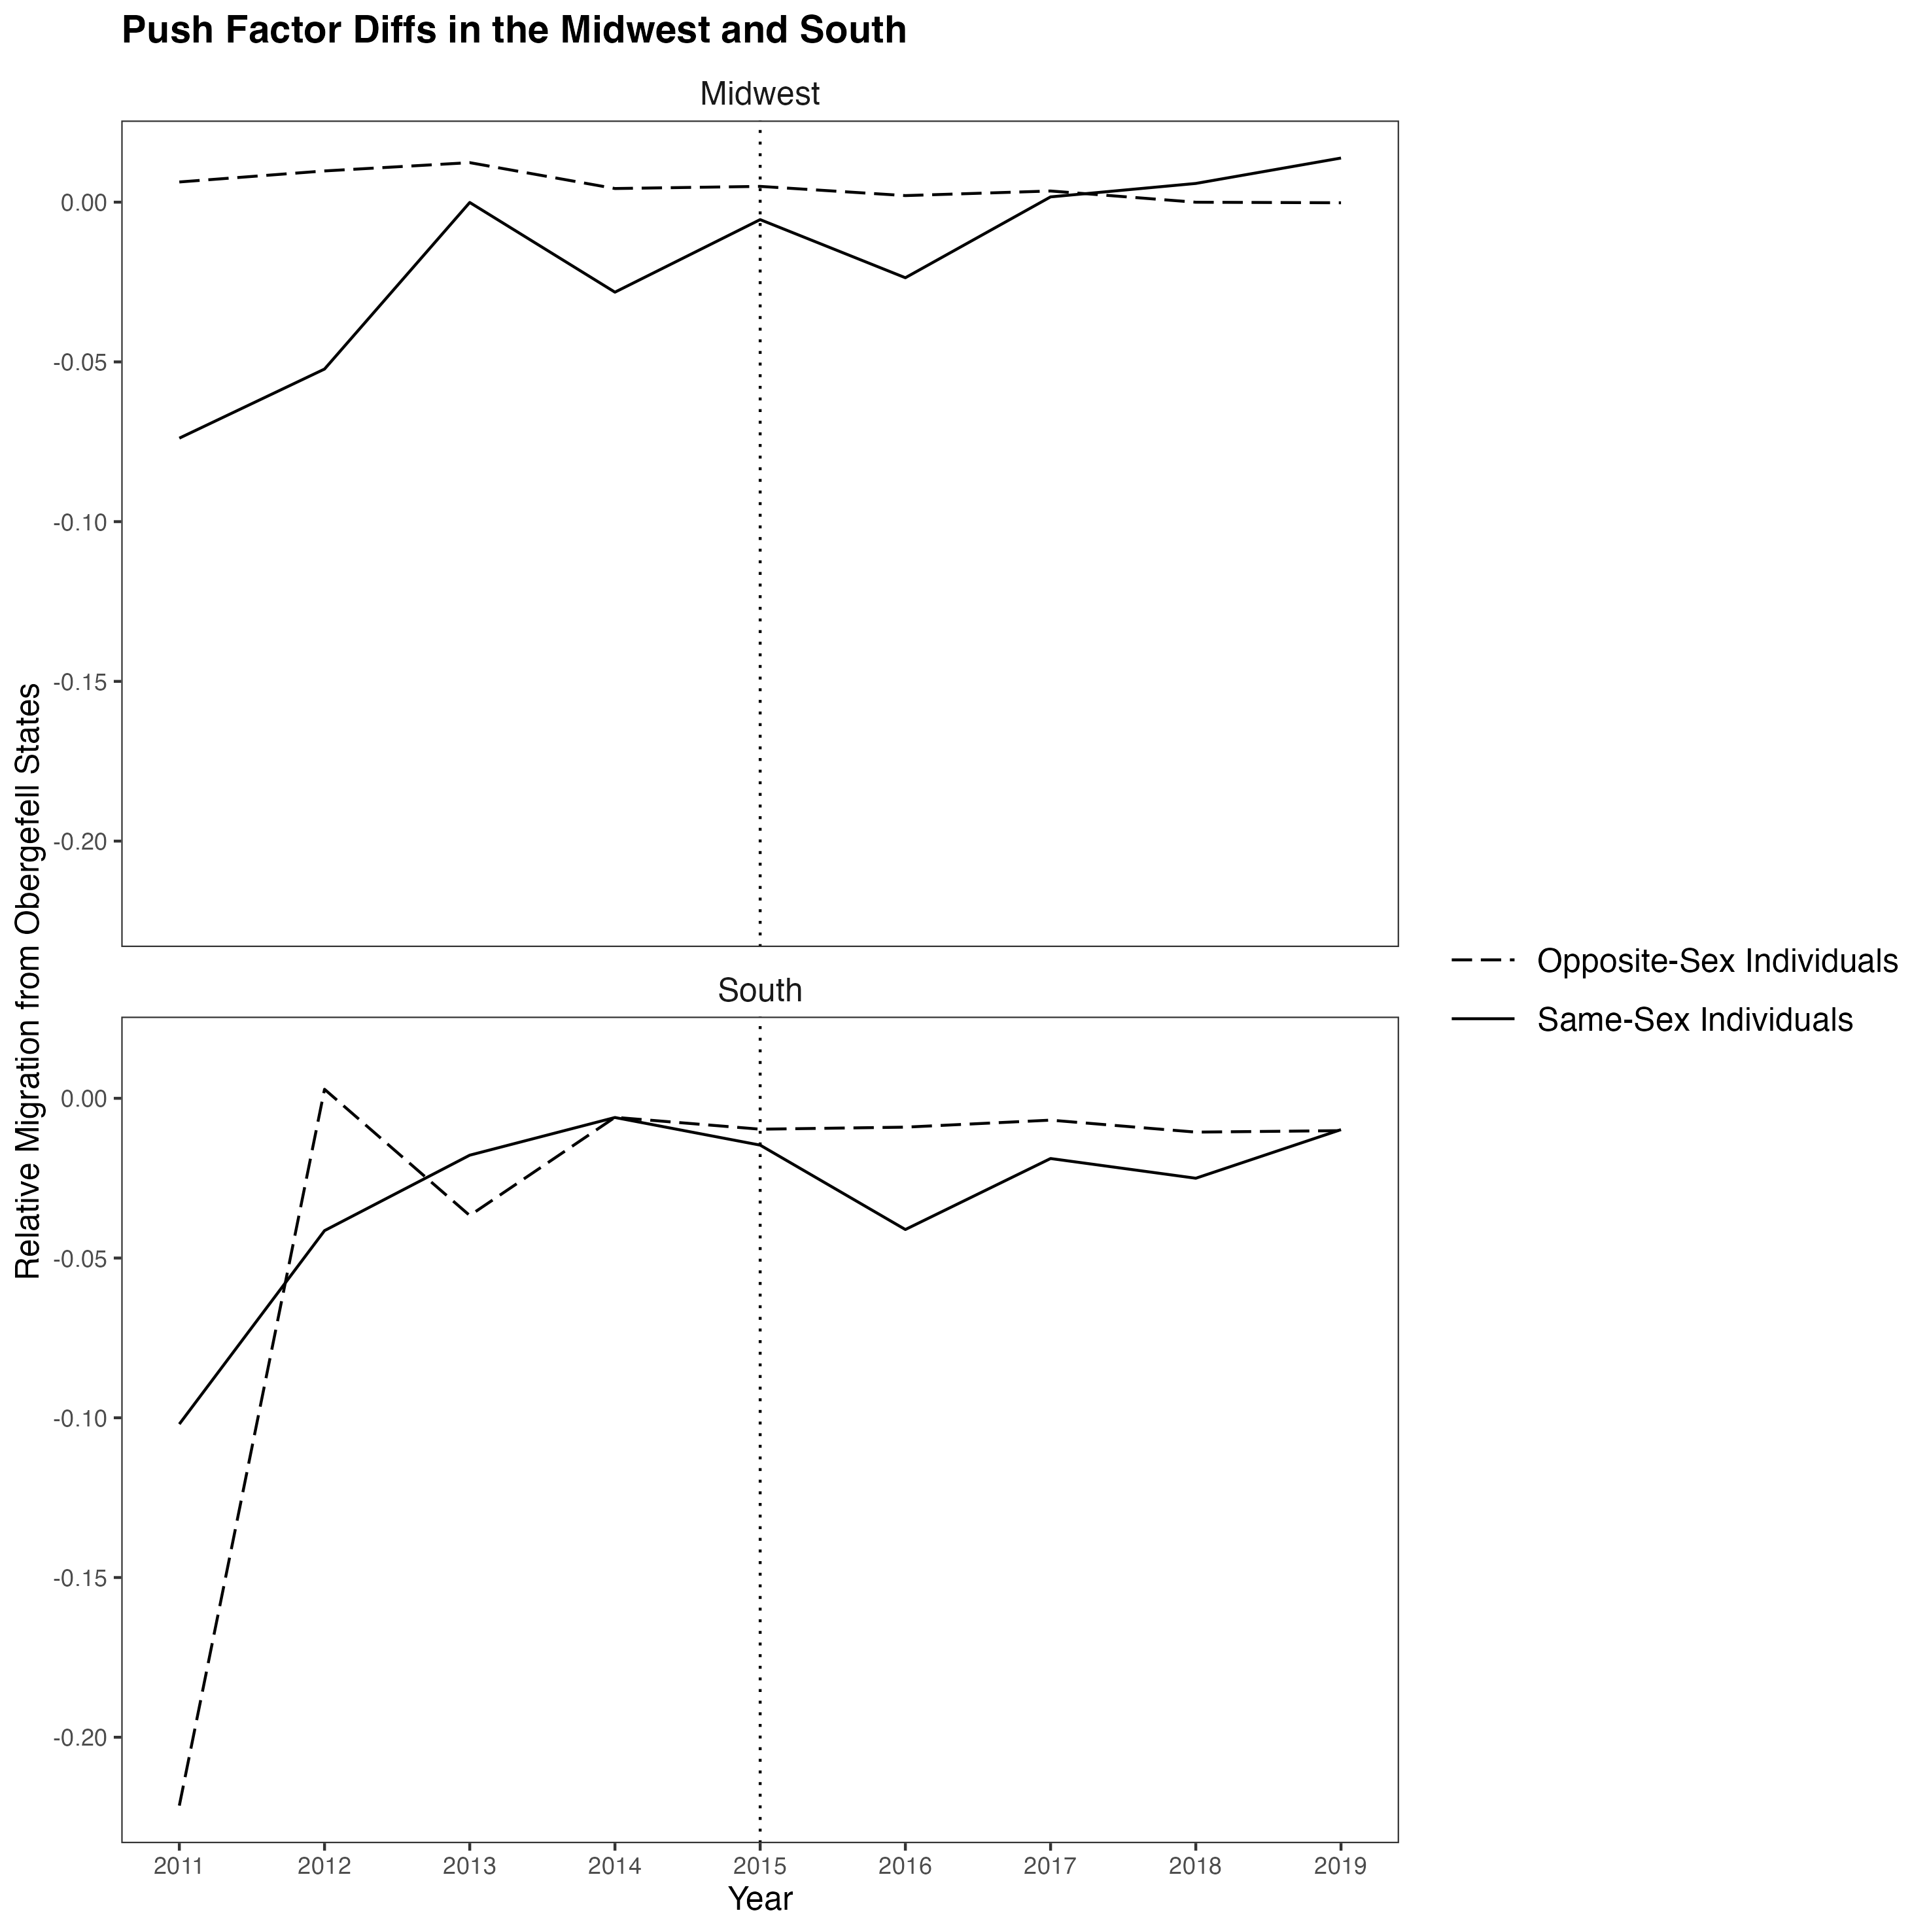
\includegraphics[width=1\linewidth]{outputs/summary_stats/region_ante_diffs.png}
    \caption{}
    \label{fig: region_ante_diffs}
\end{figure}

\floatBarrier
%separate for south/midwest?
%add in cites
%add in more about sigs?
As figures \ref{fig: region_post_diffs} and \ref{fig: region_ante_diffs} show, parallel trends hold for the south and midwest. Like in the case of sex, this suggests that less caution need be taken in utilizing a triple difference model to understand the relationship between those in the south and midwest and marriage equality (Figures for the west and northeast can be found in the appendix). 
%say more here?
\begin{table}[htbp]
    \centering
    \caption{Pull Factor Model: South}
    \label{tab: south_expost_model}
    \begin{tabular}{lccc}
\hline
 & (1) & (2) & (3) \\
VARIABLES & Model 1 & Model 2 & Model 3 \\ \hline
 &  &  &  \\
$\hat{\beta_1}$ & 0.009 & 0.057 & 0.061 \\
 & (0.014) & (0.045) & (0.053) \\
Constant & 0.103*** & 4.433*** & 4.132*** \\
 & (0.000) & (0.289) & (0.194) \\
 &  &  &  \\
Observations & 7,073 & 7,073 & 7,073 \\
 R-squared & 0.002 & 0.919 & 0.930 \\ \hline
\multicolumn{4}{c}{ Robust standard errors in parentheses} \\
\multicolumn{4}{c}{ *** p$<$0.01, ** p$<$0.05, * p$<$0.1} \\
\multicolumn{4}{p{0.6\linewidth}}{\footnotesize Column 1 reports the regression coefficient of a model with state, year, and relationship-type fixed effects including corresponding interactions; column 2 reports the regression coefficient of a model with these fixed effects and controls for sex, race, education level, the presence of children in the household, income level, and age; and column 3 reports the regression coefficients of a model with these fixed effects, controls, and controls for an individual’s birth state.} \\
\end{tabular}

\end{table}
\begin{table}[htbp]
    \centering
    \caption{Pull Factor Model: Midwest}
    \label{tab: midwest_expost_model}
    \begin{tabular}{lccc}
\hline
 & (1) & (2) & (3) \\
VARIABLES & Model 1 & Model 2 & Model 3 \\ \hline
 &  &  &  \\
$\hat{\beta_1}$ & 0.011 & -0.003 & -0.003 \\
 & (0.017) & (0.062) & (0.057) \\
Constant & 0.080*** & 3.771*** & 3.405*** \\
 & (0.000) & (0.126) & (0.369) \\
 &  &  &  \\
Observations & 4,486 & 4,486 & 4,486 \\
 R-squared & 0.002 & 0.940 & 0.942 \\ \hline
\multicolumn{4}{c}{ Robust standard errors in parentheses} \\
\multicolumn{4}{c}{ *** p$<$0.01, ** p$<$0.05, * p$<$0.1} \\
\multicolumn{4}{p{0.8\linewidth}}{\small Column 1 reports the regression coefficient of a model with state, year, and relationship-type fixed effects including corresponding interactions; column 2 reports the regression coefficient of a model with these fixed effects and controls for sex, race, education level, the presence of children in the household, income level, and age; and column 3 reports the regression coefficients of a model with these fixed effects, controls, and controls for an individual’s birth state.} \\
\end{tabular}

\end{table}
Similar to the main model, pull factor column 3 coefficients are positive and statistically insignificant. However, they are larger in magnitude with a relatively smaller confidence interval. Pull factor column 3 coefficients for the midwest are small and statistically insignificant (although positive in column 1).  As in the main model, the 95 percent confidence interval includes the null result. This suggests there is some evidence more individuals in same-sex relationships moved to southern \textit{Obergefell}-legalized states after 2015, but less moved to midwestern \textit{Obergefell}-legalized states after 2015. This could be related to regional migration trends as a whole, as migration to the South has increased while migration to the Midwest has declined since 2015 (CITE). 

\begin{table}[htbp] %finagling to get formatting to work
    \centering
    \caption{Push Factor Model: South}
    \label{tab: south_exante_model}
    \begin{tabular}{lccc}
\multicolumn{4}{c}{Ex-Ante Model: South} \\ \hline
 & (1) & (2) & (3) \\
VARIABLES & Model 1 & Model 2 & Model 3 \\ \hline
 &  &  &  \\
ante\_treatment & 0.003 & 0.061 & 0.057 \\
 & (0.017) & (0.045) & (0.046) \\
Constant & 0.100*** & 4.092*** & 4.012*** \\
 & (0.000) & (0.127) & (0.156) \\
 &  &  &  \\
Observations & 6,807 & 6,807 & 6,807 \\
 R-squared & 0.002 & 0.934 & 0.937 \\ \hline
\multicolumn{4}{c}{ Robust standard errors in parentheses} \\
\multicolumn{4}{c}{ *** p$<$0.01, ** p$<$0.05, * p$<$0.1} \\
\multicolumn{4}{c}{ See below.} \\
\end{tabular}

\end{table}
\begin{table}[htbp] %finagling to get formatting to work
    \centering
    \caption{Push Factor Model: Midwest}
    \label{tab: midwest_exante_model}
    \begin{tabular}{lccc}
\multicolumn{4}{c}{Ex-Ante Model: Midwest} \\ \hline
 & (1) & (2) & (3) \\
VARIABLES & Model 1 & Model 2 & Model 3 \\ \hline
 &  &  &  \\
ante\_treatment & 0.003 & -0.017 & 0.004 \\
 & (0.017) & (0.046) & (0.048) \\
Constant & 0.095*** & 4.167*** & 4.651*** \\
 & (0.000) & (0.159) & (0.367) \\
 &  &  &  \\
Observations & 4,684 & 4,684 & 4,684 \\
 R-squared & 0.002 & 0.917 & 0.924 \\ \hline
\multicolumn{4}{c}{ Robust standard errors in parentheses} \\
\multicolumn{4}{c}{ *** p$<$0.01, ** p$<$0.05, * p$<$0.1} \\
\end{tabular}

\end{table}

Similar to the main model, push factor column 3 coefficients for the south and midwest are positive and statistically insignificant (although negative for column 2 for the midwest). Like above, however, the southern coefficient is noticeably larger with a relatively smaller confidence interval. This suggests there is some evidence more individuals in same-sex relationships moved out of southern and midwestern \textit{Obergefell}-legalized states after 2015. Consistent with the main model, this then suggests that there could have been an in-state reaction to marriage equality less visible outside the \textit{Obergefell}-legalized states in these regions. These results would also suggest this effect was more pronounced in the south than the midwest.
%would be cool to pull in outside evidence of laws/blowback in these regions


\FloatBarrier
\subsection{Flow Heterogeneity}

%WEAKEST SECTION - KEEP THINKING- and update corresponding sections as needed

%give section new name?
%put this after popular support?
%sigh clarity what I’m actually testing for…see empirical section 3 outcomes put in somewhere above
In the main model, I follow \citet{1} and \citet{12} and do not differentiate between migration from \textit{Obergefell}- and non-\textit{Obergefell}- legalized states in the pull model and migration to \textit{Obergefell}- and non-\textit{Obergefell}- legalized states in the push model.  In my discussion of these results, I suggest that the differing effects of \textit{Obergefell v. Hodges} as a push and pull factor respectively may stem from how individuals in \textit{Obergefell}-legalized states perceive these states compared to those living in non-\textit{Obergefell}-legalized states.  In this section, I test this theory using flow heterogeneity.  Specifically, I test whether individuals from states that had legalized same-sex marriage earlier were more likely to move to \textit{Obergefell}-legalized states after 2015, and whether individuals from \textit{Obergefell}-legalized states were more likely to move to states that legalized earlier, after 2015.
%better

\begin{table}[htbp]
    \centering
    \caption{Pull Factor Model: From a State that Legalized Before 2015}
    \label{tab: flocal_expost_model}
    \begin{tabular}{lccc}
\hline
 & (1) & (2) & (3) \\
VARIABLES & Model 1 & Model 2 & Model 3 \\ \hline
 &  &  &  \\
post\_treatment & 0.025** & 0.015 & 0.004 \\
 & (0.011) & (0.023) & (0.030) \\
Constant & 0.000*** & 2.095*** & 2.102*** \\
 & (0.000) & (0.350) & (0.352) \\
 &  &  &  \\
Observations & 19,755 & 19,755 & 19,755 \\
 R-squared & 0.046 & 0.511 & 0.548 \\ \hline
\multicolumn{4}{c}{\small Robust standard errors in parentheses} \\
\multicolumn{4}{c}{\small *** p$<$0.01, ** p$<$0.05, * p$<$0.1} \\
\multicolumn{4}{p{0.8\linewidth}}{\small Column 1 reports the
regression coefficient of a model with only state and year fixed effects; column 2 reports the
regression coefficient of a model with these fixed effects and controls for sex, race, education
level, the presence of children in the household, income level, and age; and column 3 reports
the regression coefficients of a model with these fixed effects, controls, and controls for an
individual’s birth state.} \\
\end{tabular}

\end{table}
\begin{table}[htbp] %finagling to get formatting right
    \centering
    \caption{Push Factor Model: To a State that Legalized Before 2015}
    \label{tab: tlocal_exante_model}
    \begin{tabular}{lccc}
\multicolumn{4}{c}{To Locally Legalized} \\ \hline
 & (1) & (2) & (3) \\
VARIABLES & Model 1 & Model 2 & Model 3 \\ \hline
 &  &  &  \\
ante\_treatment & -0.024** & -0.020 & -0.012 \\
 & (0.010) & (0.023) & (0.031) \\
Constant & 0.001*** & 2.048*** & 2.110*** \\
 & (0.000) & (0.348) & (0.368) \\
 &  &  &  \\
Observations & 19,755 & 19,755 & 19,755 \\
 R-squared & 0.048 & 0.516 & 0.541 \\ \hline
\multicolumn{4}{c}{ Robust standard errors in parentheses} \\
\multicolumn{4}{c}{ *** p$<$0.01, ** p$<$0.05, * p$<$0.1} \\
\end{tabular}

\end{table}

Table \ref{tab: flocal_expost_model} displays regression results from a modified pull factor model. Instead of the outcome variable being whether an individual migrated or not, the outcome variable is if an individual migrated from a state that had legalized same-sex marriage before \textit{Obergefell v. Hodges} or not. Table \ref{tab: tlocal_exante_model} displays regression results from a modified push factor model. Instead of the outcome variable being whether an individual migrated or not, the outcome variable is if an individual migrated to a state that had legalized same-sex marriage before \textit{Obergefell v. Hodges} or not. Further specifications- covering the from and to \textit{Obergefell}-legalized cases- can be found in the appendix (tables \ref{tab: ffed_expost_model} and \ref{tab: tfed_exante_model}).

\begin{figure}[htbp]
    \centering
    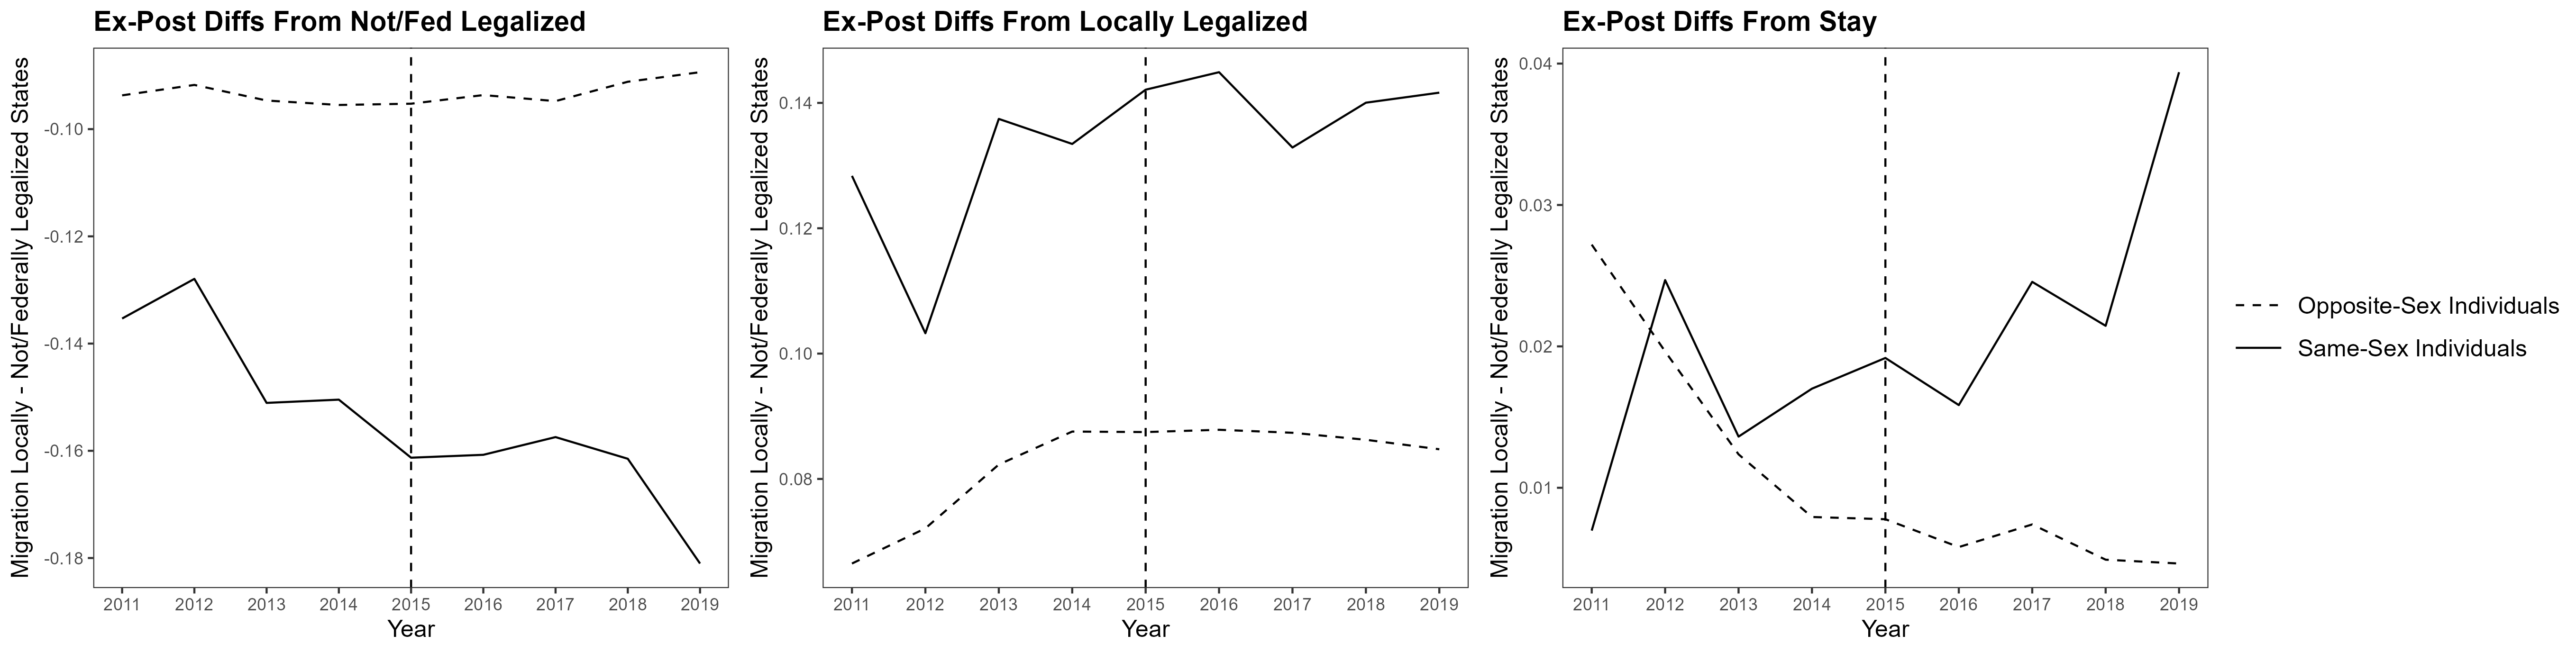
\includegraphics[width=1\linewidth]{outputs/summary_stats/flows_post_diffs.png}
    \caption{}
    \label{fig: flows_post_diffs}
\end{figure}
\begin{figure}[htbp]
    \centering
    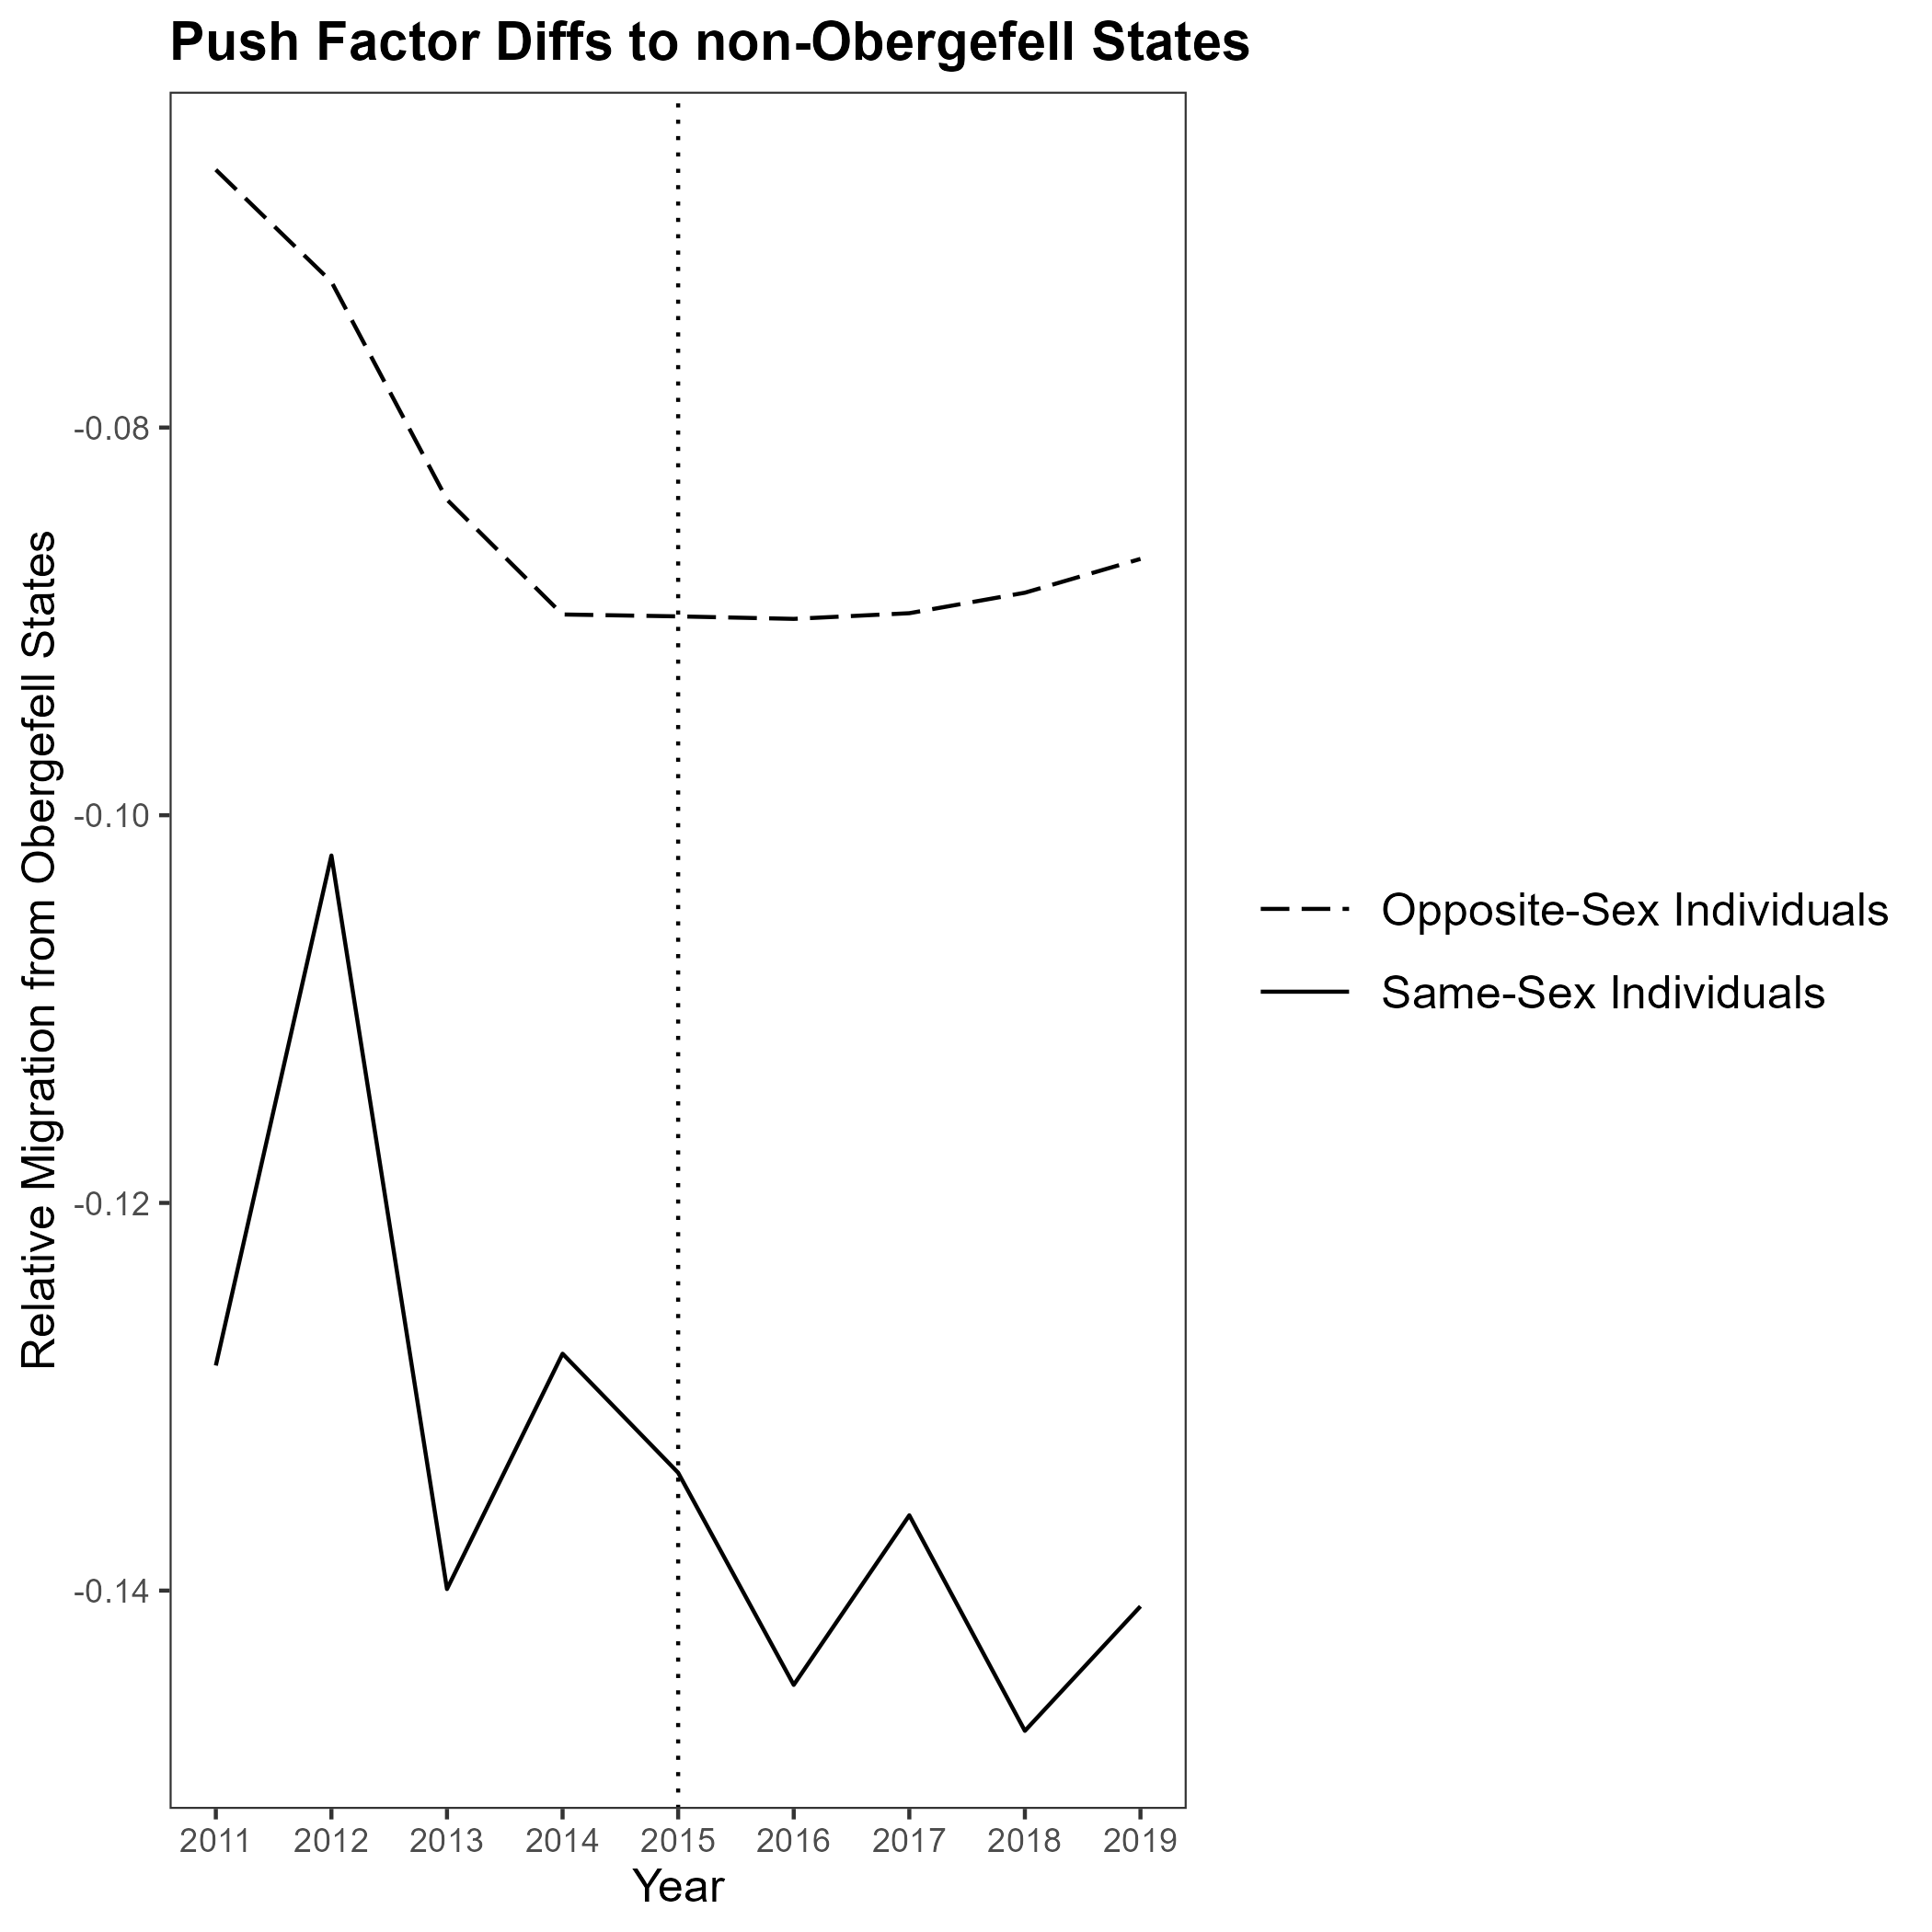
\includegraphics[width=1\linewidth]{outputs/summary_stats/flows_ante_diffs.png}
    \caption{}
    \label{fig: flows_ante_diffs}
\end{figure}

%need to update figures
Figures \ref{fig: flows_post_diffs} and \ref{fig: flows_post_diffs} illustrate that parallel trends hold to some degree (figures for the other models can be found in the appendix). This suggests that underlying trends are obfuscated to some degree in the main model by migration source or destination heterogeneity. The pull factor column 3 coefficient is negative and statistically insignificant (however, the column 1 coefficient is). The 95 percent confidence interval includes the null result. This implies that fewer individuals migrated from non-\textit{Obergefell}-legalized states to \textit{Obergefell}-legalized states after 2015.  Similarly, the push factor column 3 coefficient is negative and statistically insignificant (however, the column 1 coefficient is). The 95 percent confidence interval includes the null result. However, it is relatively large. This implies that fewer individuals migrated to \textit{Obergefell}-legalized states from non-\textit{Obergefell}-legalized states after 2015. Together, these results contradict my earlier theory. Perhaps, other differences between these state types keep individuals from moving between them.

%WEAKEST SECTION - KEEP THINKING

\FloatBarrier
\subsection{Social Acceptance}

While I include state fixed effects in my model, I do not explicitly account for the level of popular support for gay people in each state. If there are varying levels of popular support for gay people across \textit{Obergefell}- legalized states, that could also complicate the analysis of the effect of \textit{Obergefell v. Hodges}. If gay people have less popular support, that could obfuscate the effect of \textit{Obergefell}-legalization.
%improve connection to material

\begin{spacing}{1}
\begin{longtable}{|c|c|}
\caption{Support for Gay Men and Lesbian Women by State in 2016}
\label{tab: pop_support}
\hline
\textbf{State} & \textbf{Popular Support}\\
\hline
Alaska & 40\\
North Dakota & 45\\
Alabama & 46\\
Maine & 48\\
West Virginia & 48\\
Arkansas & 49\\
Oklahoma & 50\\
Virginia & 51\\
South Carolina & 51\\
Texas & 52\\
South Dakota & 52\\
Mississippi & 52\\
Ohio & 53\\
Indiana & 54\\
Tennessee & 54\\
Missouri & 55\\
North Carolina & 55\\
Georgia & 56\\
Iowa & 56\\
Nebraska & 57\\
Maryland & 58\\
Louisiana & 58\\
Michigan & 58\\
Florida & 59\\
Kentucky & 59\\
Montana & 59\\
Idaho & 60\\
Kansas & 60\\
Wisconsin & 61\\
Illinois & 61\\
Colorado & 61\\
Nevada & 62\\
Pennsylvania & 62\\
Utah & 62\\
Minnesota & 62\\
New Mexico & 62\\
Arizona & 63\\
Rhode Island & 63\\
Hawaii & 64\\
Washington & 64\\
Delaware & 64\\
California & 69\\
New Jersey & 70\\
New York & 70\\
Oregon & 70\\
Connecticut & 71\\
Wyoming & 72\\
Vermont & 72\\
Massachusetts & 76\\
New Hampshire & 77\\
District of Columbia & 83\\
\hline
\multicolumn{2}{p{0.8\linewidth}}{\small \textbf{Note:} Support levels represent a weighted average of responses to the question: "How would you rate gay men and lesbians?" Values closer to 100 indicate \textit{more} support; values closer to 0 indicate \textit{less} support.} \\ 
\end{longtable}
\end{spacing}


Table \ref{tab: pop_support} displays state-wide support for individuals in same-sex relationships in 2016. Larger values indicate less support while smaller values indicate more support. Data comes from \citet{29}. In the following regressions, I interact this measure for popular support with the triple difference term from my main model. I do not include popular support as a separate control as popular support should be captured by state-fixed effects.

\hfill
\break
%<pull eqn>
Social Acceptance Pull Factor Regression:
\begin{equation}
\begin{aligned}
\text{m}_{itg} &= \gamma_t + \gamma_g + \gamma_s + \gamma_{tg} + \gamma_{ts} + \gamma_{sg} \\
&\quad + \beta_1 \cdot (\text{support}_g \times \text{samesex}_i \times \text{post2015}_t \times \text{Obergefell legalized}_g) \\
&\quad + X_{it} + \epsilon_{itg}
\end{aligned}
\end{equation}

\hfill
\break
Social Acceptance Push Factor Regression:
\begin{equation}
\begin{aligned}
\text{m}_{ith} &= \gamma_t + \gamma_h + \gamma_s + \gamma_{th} + \gamma_{ts} + \gamma_{sh} \\
&\quad + \beta_2 \cdot (\text{support}_h \times \text{samesex}_i \times \text{post2015}_t \times \text{Obergefell legalized}_h) \\
&\quad + X_{it} + \epsilon_{ith}
\end{aligned}
\end{equation}

Table \ref{tab: popsupport_expost_model} reports results from the social acceptance pull factor model. Similar to the main model, the column 3 coefficient is positive and statistically insignificant. The 95 percent confidence interval includes the null result. Unlike the main model, the column 3 coefficient is significantly larger. Table \ref{tab: popsupport_exante_model} reports results from the social acceptance push factor model. Similar patterns hold as in the pull model. This implies that relatively more same-sex individuals move to a \textit{Obergefell}-legalized state after 2015 when the state has more support for gay people. However, this also implies relatively more same-sex individuals leave a \textit{Obergefell}-legalized state after 2015 when the state has more support for gay people. 

\begin{table}[htbp] %maybe put on top
    \centering
    \caption{Pull Factor Model: Popular Support}
    \label{tab: popsupport_expost_model}
    \begin{tabular}{lccc}
\multicolumn{4}{c}{Ex-Post Model - Anti Popular Support} \\ \hline
 & (1) & (2) & (3) \\
VARIABLES & Model 1 & Model 2 & Model 3 \\ \hline
 &  &  &  \\
post\_treatment & 0.019 & 0.010 & 0.010 \\
 & (0.013) & (0.047) & (0.055) \\
Constant & 0.103*** & 4.063*** & 3.913*** \\
 & (0.000) & (0.131) & (0.108) \\
 &  &  &  \\
Observations & 19,755 & 19,755 & 19,755 \\
 R-squared & 0.005 & 0.922 & 0.927 \\ \hline
\multicolumn{4}{c}{ Robust standard errors in parentheses} \\
\multicolumn{4}{c}{ *** p$<$0.01, ** p$<$0.05, * p$<$0.1} \\
\multicolumn{4}{p{0.8\linewidth}}{\small Column 1 reports the
regression coefficient of a model with only state and year fixed effects; column 2 reports the
regression coefficient of a model with these fixed effects and controls for sex, race, education
level, the presence of children in the household, income level, and age; and column 3 reports
the regression coefficients of a model with these fixed effects, controls, and controls for an
individual’s birth state.} \\
\end{tabular}

\end{table}
\begin{table}[htbp]
    \centering
    \caption{Push Factor Model: Popular Support}
    \label{tab: popsupport_exante_model}
    \begin{tabular}{lccc}
\multicolumn{4}{c}{Ex-Ante Model - Popular Support} \\ \hline
 & (1) & (2) & (3) \\
VARIABLES & Model 1 & Model 2 & Model 3 \\ \hline
 &  &  &  \\
$\hat{\beta_2}$ & 0.012 & 0.015 & 0.011 \\
 & (0.016) & (0.043) & (0.044) \\
Constant & 0.100*** & 4.142*** & 4.087*** \\
 & (0.000) & (0.084) & (0.108) \\
 &  &  &  \\
Observations & 19,755 & 19,755 & 19,755 \\
 R-squared & 0.004 & 0.919 & 0.921 \\ \hline
\multicolumn{4}{c}{ Robust standard errors in parentheses} \\
\multicolumn{4}{c}{ *** p$<$0.01, ** p$<$0.05, * p$<$0.1} \\
\multicolumn{4}{p{0.8\linewidth}}{\small Column 1 reports the regression coefficient of a model with state, year, and relationship-type fixed effects including corresponding interactions; column 2 reports the regression coefficient of a model with these fixed effects and controls for sex, race, education level, the presence of children in the household, income level, and age; and column 3 reports the regression coefficients of a model with these fixed effects, controls, and controls for an individual’s birth state.} \\
\end{tabular}

\end{table}

These results should be held with caution like all of my results; further, like the main model, parallel trends does not hold. However, this result simply implies that legalization and popular support capture similar phenomena, both of which (albeit weakly) relate to the idea that after 2015, more individuals in same-sex relationships relatively moved to \textit{Obergefell}-legalized states and left \textit{Obergefell} legalized states.
%ok I got tired and this got messy, re-read and unify later

\FloatBarrier %hmm float issues with this
\section{Conclusion}

In this paper, I investigated to what extent migration patterns of individuals in same-sex and different-sex relationships converged after 2015. I did this by comparing migration trends to and from states that independently legalized same-sex marriage before 2015 with those where legalization was federally mandated by \textit{Obergefell v. Hodges}. I added to the literature by specifically addressing \textit{Obergefell} legalization, and whether it affected holdout states differently than earlier legalization affected early adopters.
%is differently the right way to phrase this?
%does intro need to harp on what is novel more?

Using a triple differences empirical design, I found that individuals in same-sex relationships were more likely to move to states with federally-mandated marriage equality after 2015, relative to individuals in different-sex relationships and states that legalized same-sex marriage earlier. However, individuals in same-sex relationships were also more likely to move out of these states after 2015. These results should be taken with caution; necessary model assumptions were not consistently met, and results were characterized by large p-values and standard errors that included the null result.
%does this mean anything?

This provides some evidence that \textit{Obergefell}-legalization made holdout states more appealing for individuals in same-sex relationships to move to, but not necessarily to stay in. This could suggest that \textit{Obergefell} legalization improved the perception of holdout states by those living outside of them, if not those living in them. However, as seen in the flow heterogeneity regressions (section 4.4), increases in migration to \textit{Obergefell}-legalized states seemed to be driven by migrants from other \textit{Obergefell}-legalized states and increases in migration out of \textit{Obergefell}-legalized states seemed to be driven by migrants moving to other \textit{Obergefell} legalized states. 

The imprecision of my results highlights the importance of future research using datasets with richer representation of same-sex couples and the broader LGBTQ+ community. There are significant limitations to using census-identified co-habiting same-sex couples to proxy same-sex couples and the broader LGBTQ+ community. There are relatively few same-sex couples identified, and those that are might not reflect same-sex couples or the LGBTQ+ community at large. The implication that \textit{Obergefell}-legalization both pulled in individuals in same-sex relationships to states and pushed them out is puzzling, and also indicates the importance of further research. This research could investigate broader migration patterns between \texit{Obergefell}-legalized and non-\textit{Obergefell}-legalized states, differences in how individuals evaluate places to move to and where they currently live, and other implications of \textit{Obergefell v. Hodges}. 
%include LGBTQ+ community here? include more numbers?
%need to justify these possible research choices?
%oi clean up comments?
%oop get at overall migration levels too

Regardless of their imprecision, these results hold important implications. There is some evidence that \textit{Obergefell v. Hodges} had an economically significant effect on individuals in same-sex relationships. This should be of note for policy makers: social policy likely has an effect on peoples' behavior. Legal rights are often seen as abstract; however, they often have tangible consequences. State leaders interested in making their states more attractive for current and future residents- and the life, business, and tax dollars they bring- should be mindful that social policy may play a role in individuals' decisions about where to live. 
%oop lost one percent discussion


Over the past twenty years, the legal landscape for individuals in same-sex relationships has changed dramatically in the United States. This has meant significant advances in civil rights, and corresponding changes in behavior. However, history is still being written. Laws and social norms affecting LGBTQ+ individuals continue to change, shaping how they live, work, and migrate. As society adapts, understanding the impact of these legal and cultural changes will continue to be important. For that, further research will continue to be useful.
%keep thinking

\newpage
% References section
\bibliographystyle{chicago}
\bibliography{Drafting/thesis_bibliography}

\newpage
\appendix
\FloatBarrier
\section{More Summary Statistics}

\begin{table}

\caption{Summary Statistics by Region (2)}
\label{region_2} %added
\centering
\begin{tabular}[t]{rrrrr}
\toprule
\multicolumn{1}{c}{ } & \multicolumn{2}{c}{\% in the West} & \multicolumn{2}{c}{\% in the Northeast} \\
\cmidrule(l{3pt}r{3pt}){2-3} \cmidrule(l{3pt}r{3pt}){4-5}
Year & Same-Sex & Opposite-Sex & Same-Sex & Opposite-Sex\\
\midrule
2011 & 27.132 & 20.213 & 19.489 & 17.055\\
2012 & 26.721 & 20.257 & 19.596 & 16.961\\
2013 & 26.781 & 20.332 & 20.001 & 16.872\\
2014 & 25.497 & 20.475 & 19.774 & 16.758\\
2015 & 26.558 & 20.576 & 19.919 & 16.620\\
\addlinespace
2016 & 27.304 & 20.784 & 18.359 & 16.411\\
2017 & 26.843 & 20.822 & 18.519 & 16.467\\
2018 & 26.159 & 21.015 & 18.721 & 16.403\\
2019 & 26.867 & 21.149 & 17.840 & 16.312\\
\bottomrule
\end{tabular}
\end{table}


\begin{landscape}
\begin{table}

\caption{Summary Statistics for Main Variables (2)}
\centering
\begin{tabular}[t]{rrrrrrrrr}
\toprule
\multicolumn{1}{c}{ } & \multicolumn{2}{c}{Mean Age} & \multicolumn{2}{c}{\% College} & \multicolumn{2}{c}{\% White} & \multicolumn{2}{c}{Mean Income} \\
\cmidrule(l{3pt}r{3pt}){2-3} \cmidrule(l{3pt}r{3pt}){4-5} \cmidrule(l{3pt}r{3pt}){6-7} \cmidrule(l{3pt}r{3pt}){8-9}
Year & Same-Sex & Opposite-Sex & Same-Sex & Opposite-Sex & Same-Sex & Opposite-Sex & Same-Sex & Opposite-Sex\\
\midrule
2011 & 46.722 & 50.049 & 99.429 & 99.483 & 86.179 & 88.156 & 50335.01 & 44533.11\\
2012 & 46.537 & 50.265 & 99.222 & 99.511 & 86.173 & 88.088 & 51139.41 & 45857.95\\
2013 & 47.561 & 50.413 & 99.229 & 99.432 & 85.612 & 87.823 & 52174.04 & 47459.77\\
2014 & 47.266 & 50.576 & 99.270 & 99.450 & 84.799 & 87.628 & 54609.46 & 48670.56\\
2015 & 47.069 & 50.759 & 99.093 & 99.464 & 84.578 & 87.558 & 54834.15 & 50661.86\\
\addlinespace
2016 & 47.122 & 50.950 & 99.160 & 99.469 & 83.841 & 87.315 & 57084.24 & 52100.23\\
2017 & 46.969 & 51.084 & 99.233 & 99.484 & 83.302 & 87.212 & 57693.76 & 53684.30\\
2018 & 46.639 & 51.164 & 99.279 & 99.479 & 82.547 & 86.968 & 58369.55 & 55735.39\\
2019 & 45.026 & 51.332 & 99.243 & 99.436 & 81.405 & 86.766 & 60204.72 & 58419.54\\
\bottomrule
\end{tabular}
\end{table}

\end{landscape}


\FloatBarrier
\newpage
\section{Additional Difference Charts}
%age
%\begin{figure}[htbp]
%    \centering
%    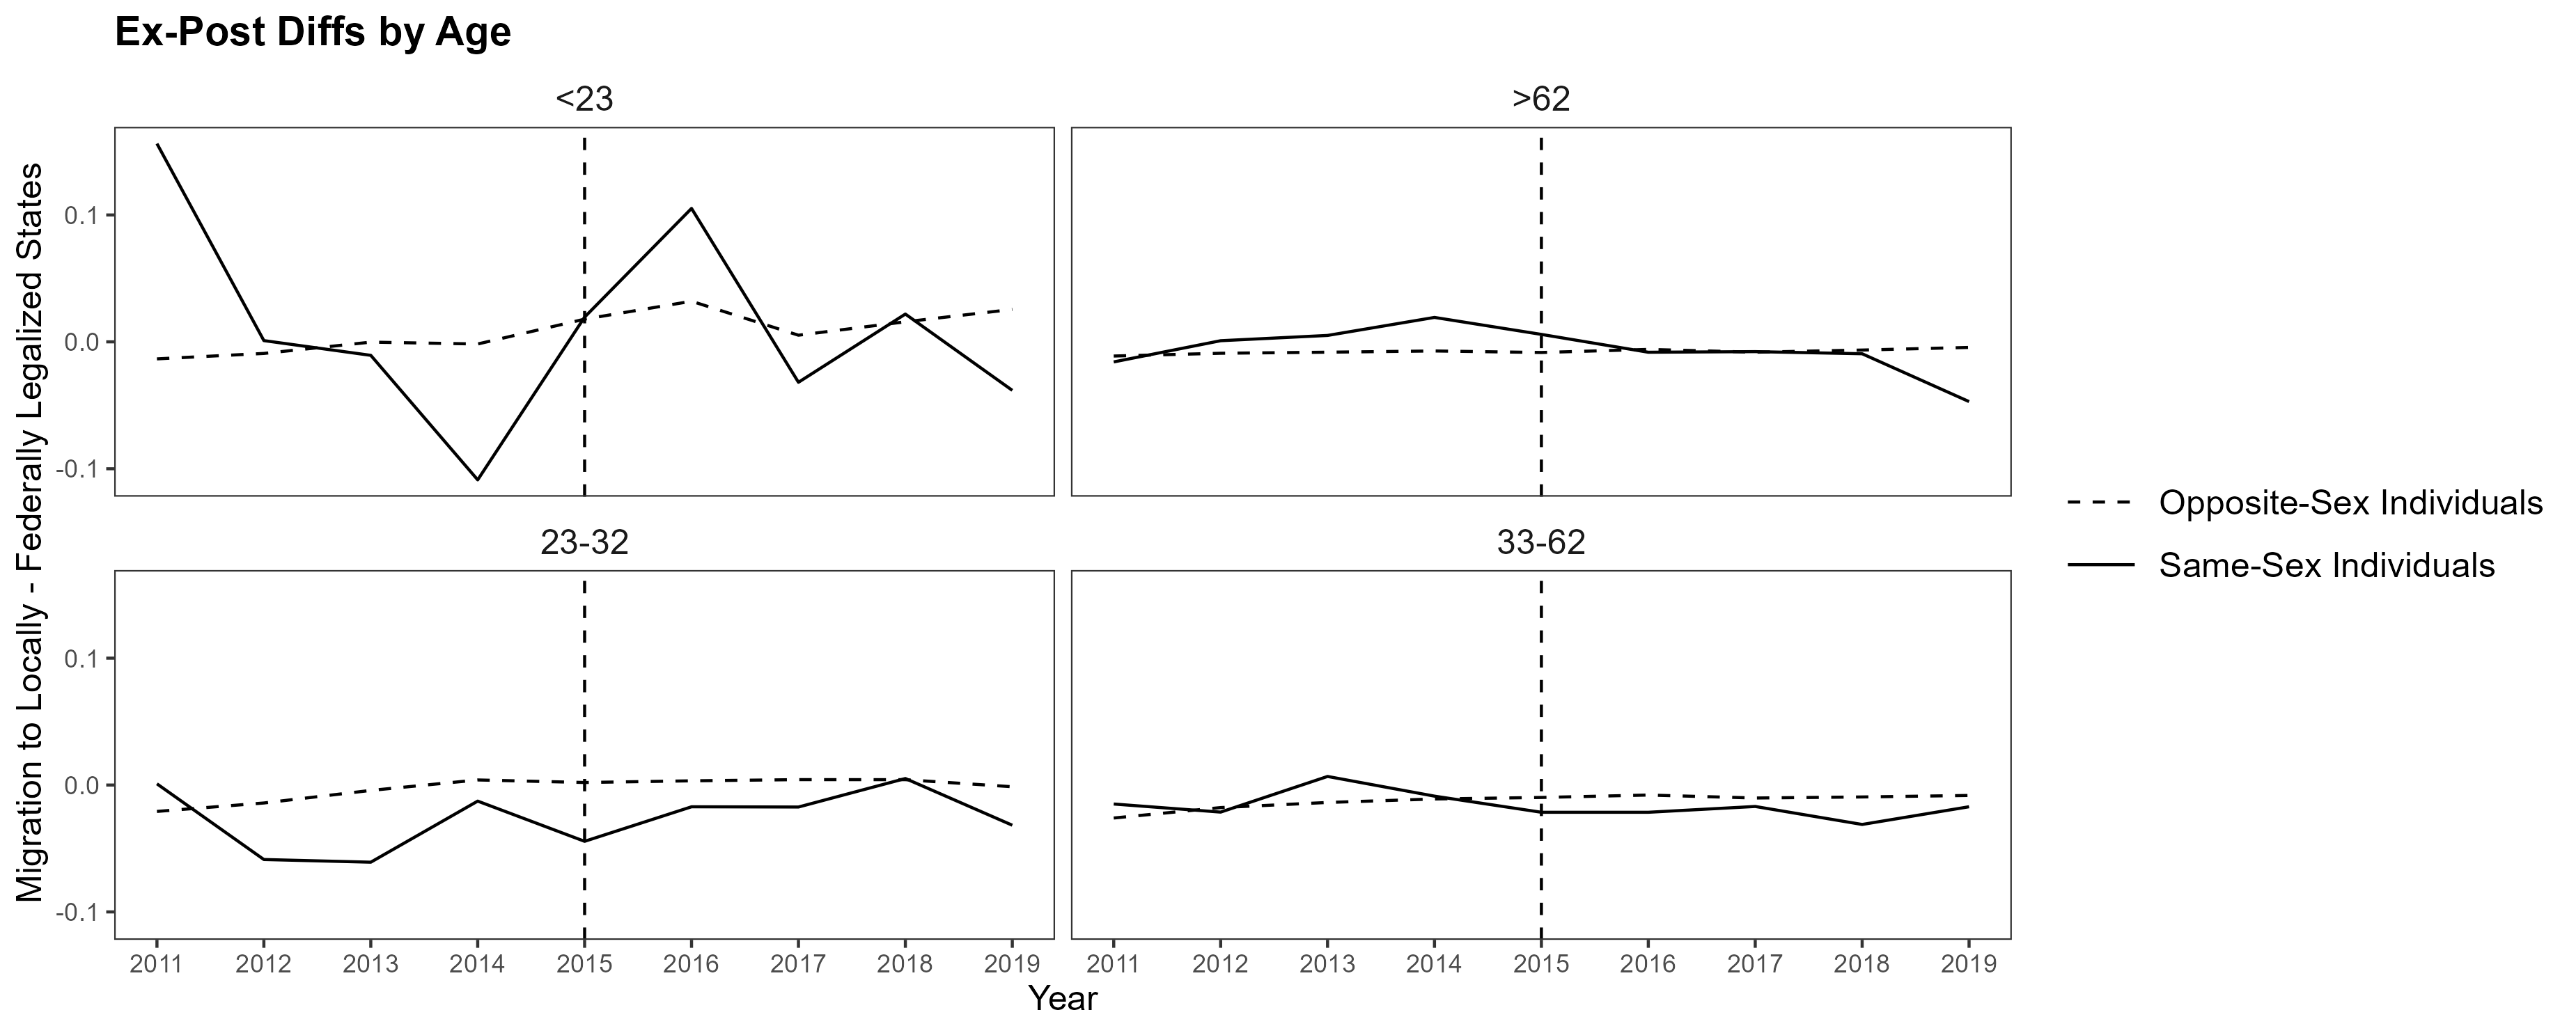
\includegraphics[width=0.75\linewidth]{outputs/summary_stats/age_post_diffs.png}
 %   \caption{}
 %   \label{}
%\end{figure}

%\begin{figure}[htbp]
%    \centering
%    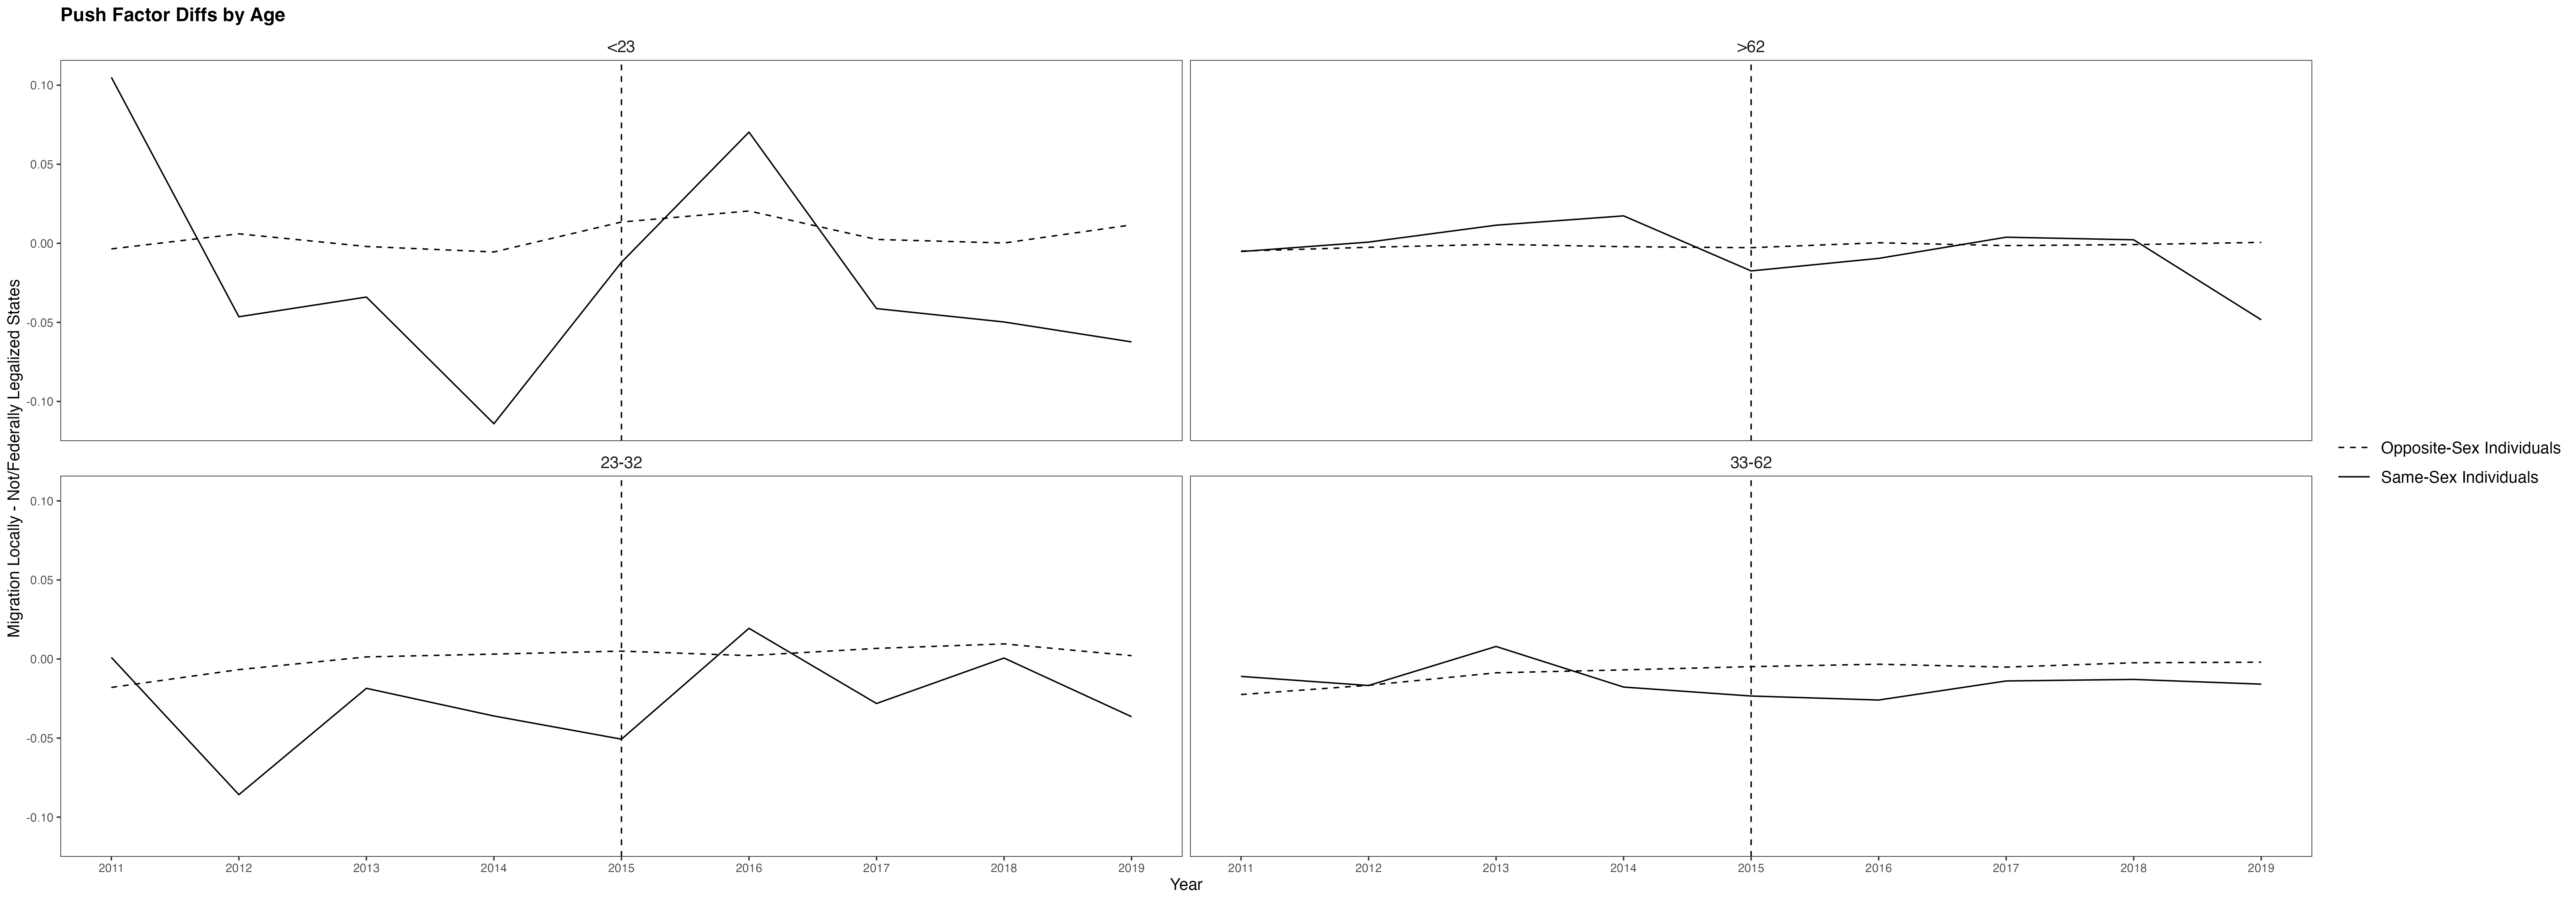
\includegraphics[width=0.75\linewidth]{outputs/summary_stats/age_ante_diffs.png}
%    \caption{}
%    \label{fig: fig:enter-label}
%\end{figure}


%child
%\begin{figure}[htbp]
%    \centering
%    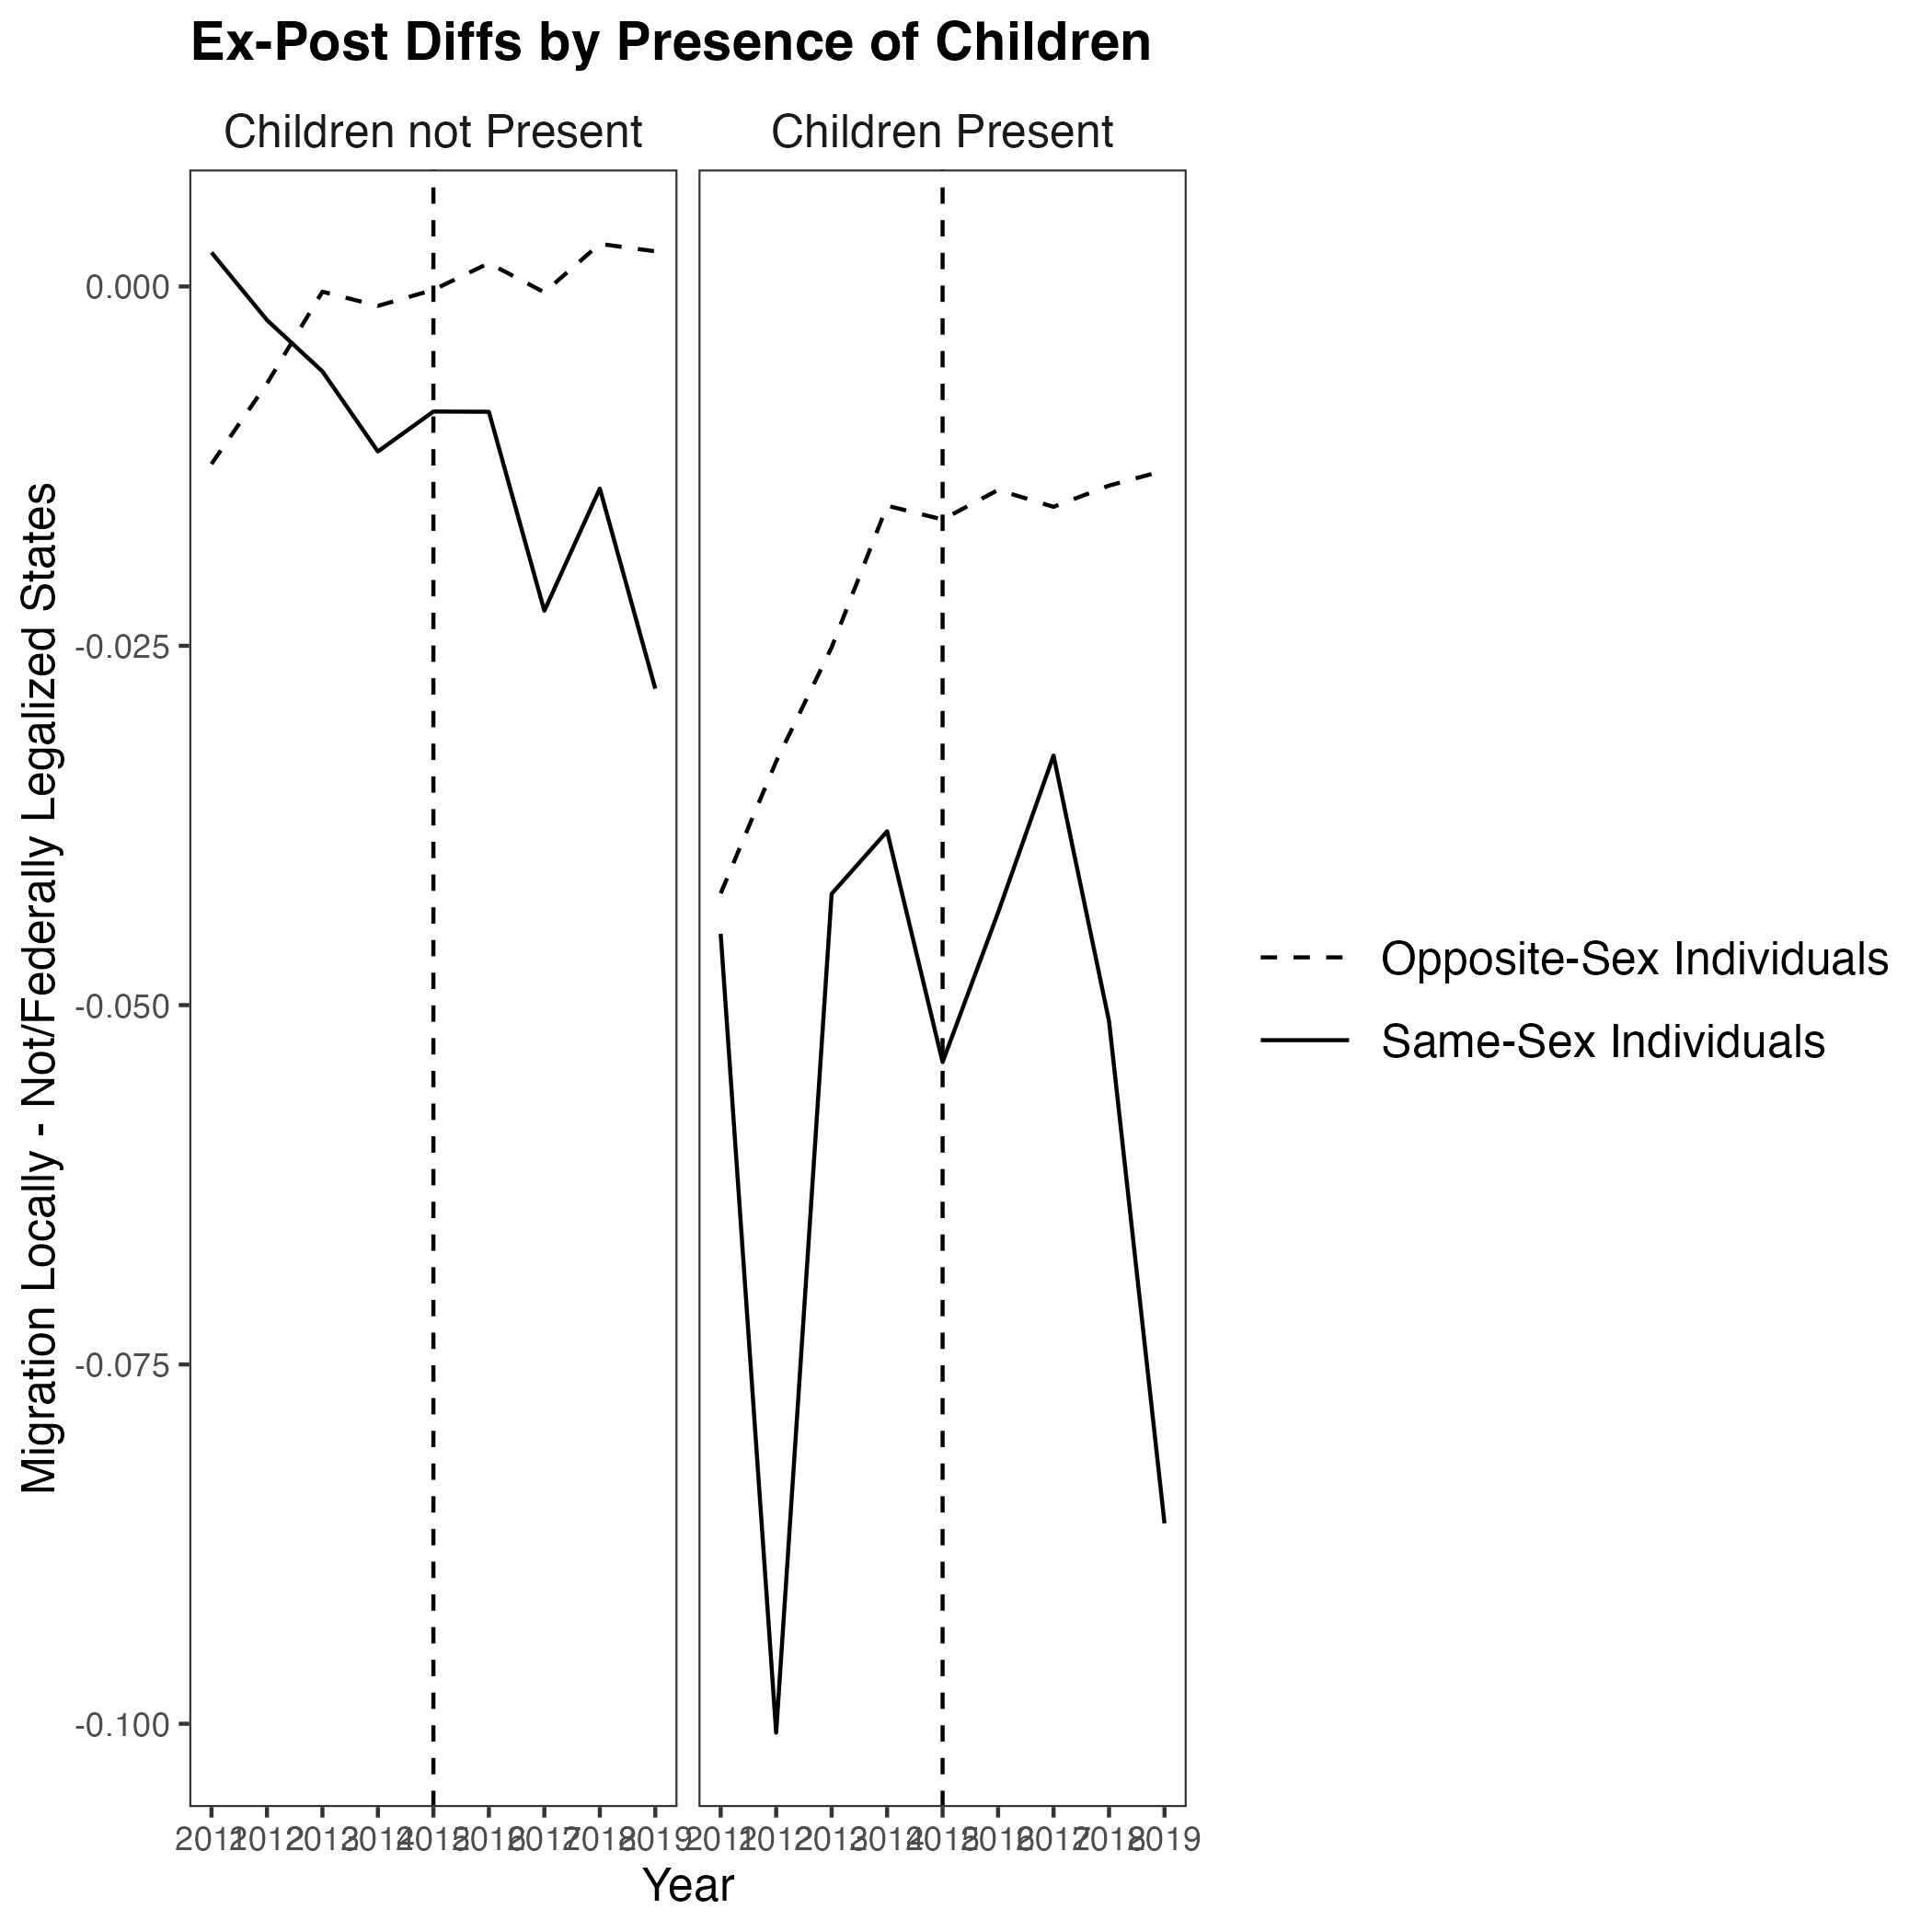
\includegraphics[width=0.75\linewidth]{outputs/summary_stats/child_post_diffs.png}
%    \caption{}
%    \label{fig: fig:enter-label}
%\end{figure}

%\begin{figure}[htbp]
%    \centering
%    \includegraphics[width=0.75\linewidth]%{outputs/summary_stats/child_ante_diffs.png}
%    \caption{}
%    \label{fig: fig:enter-label}
%\end{figure}

%Education
%\begin{figure}[htbp]
%    \centering
%    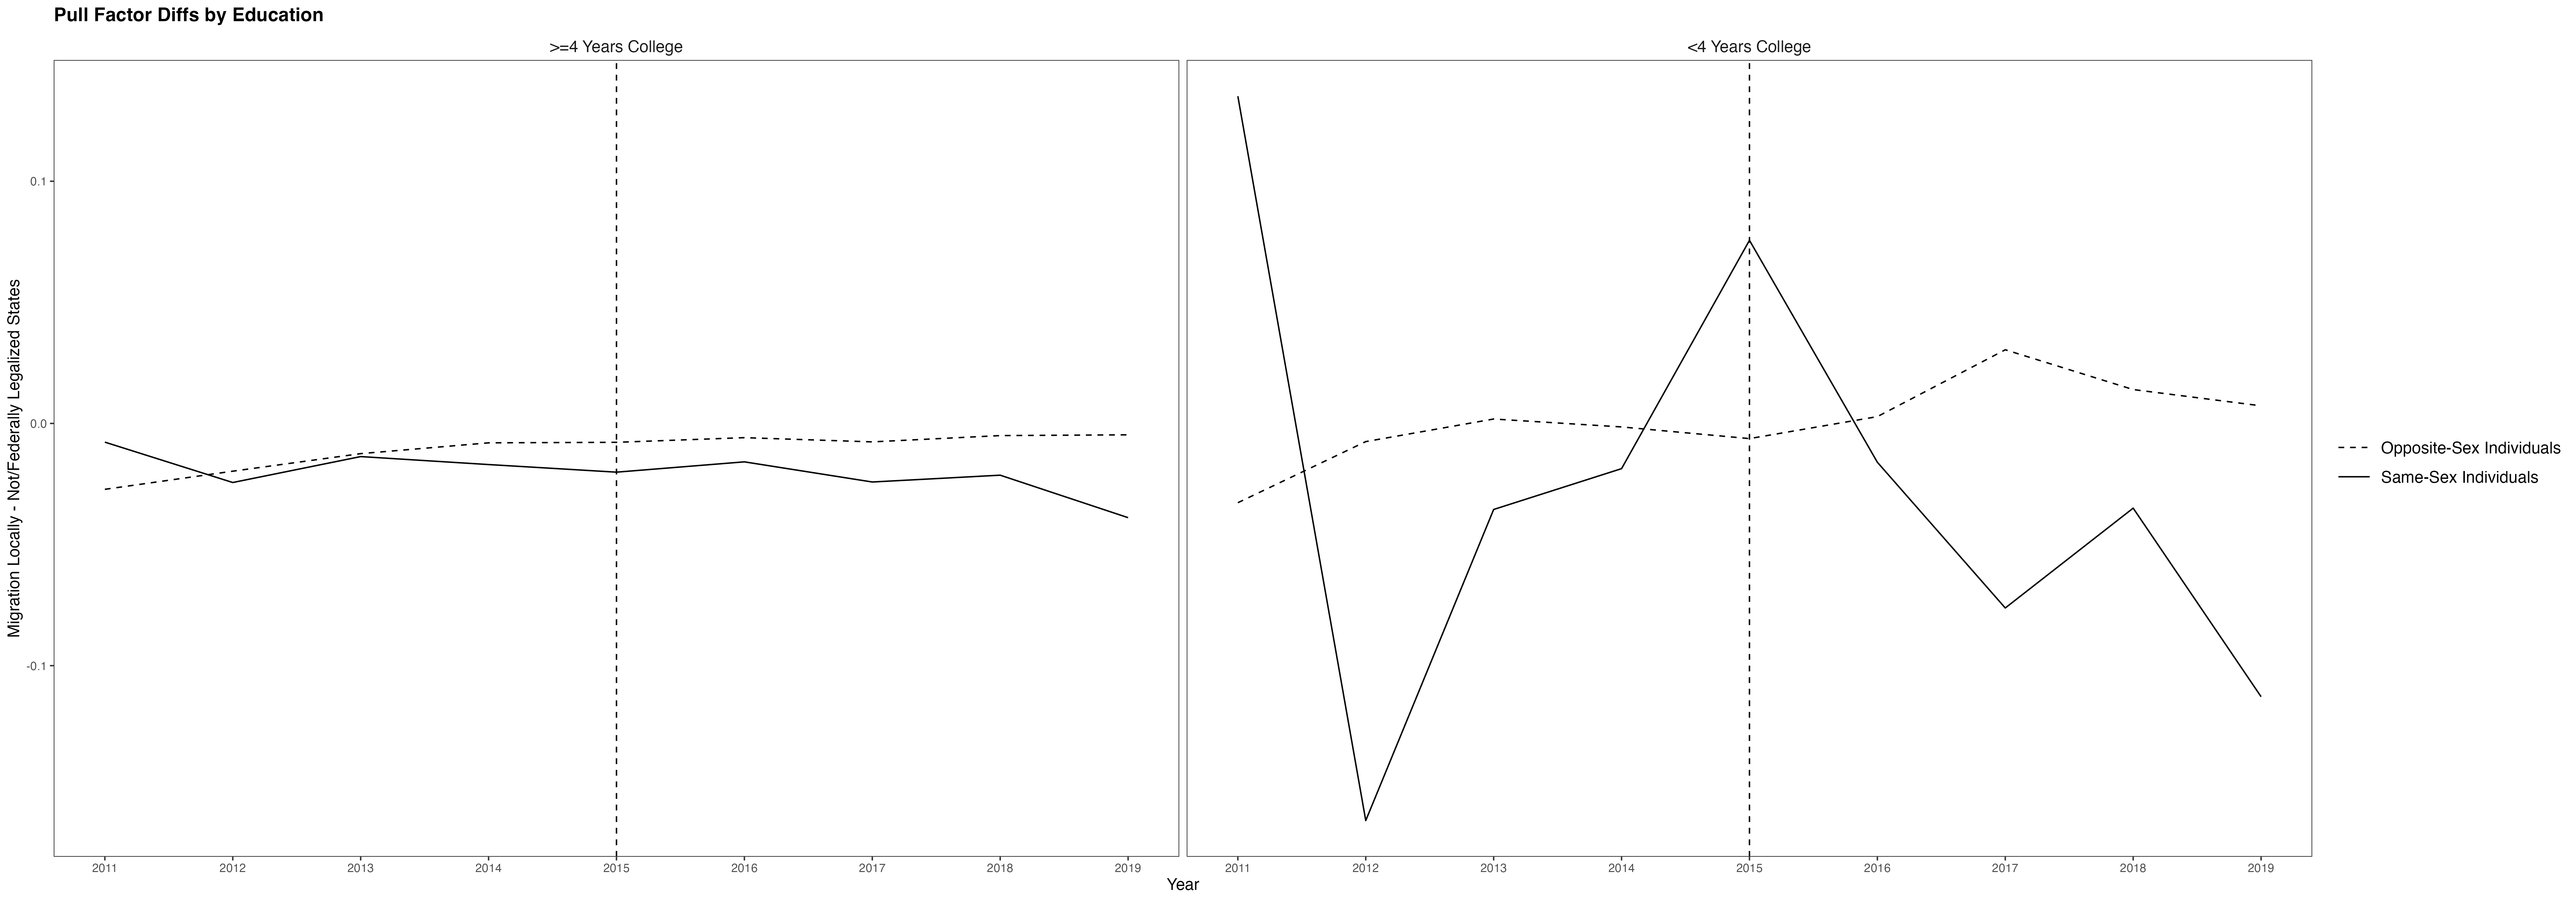
\includegraphics[width=0.75\linewidth]{outputs/summary_stats/educ_post_diffs.png}
%    \caption{}
%    \label{fig: fig:enter-label}
%\end{figure}

%\begin{figure}[htbp]
%    \centering
%    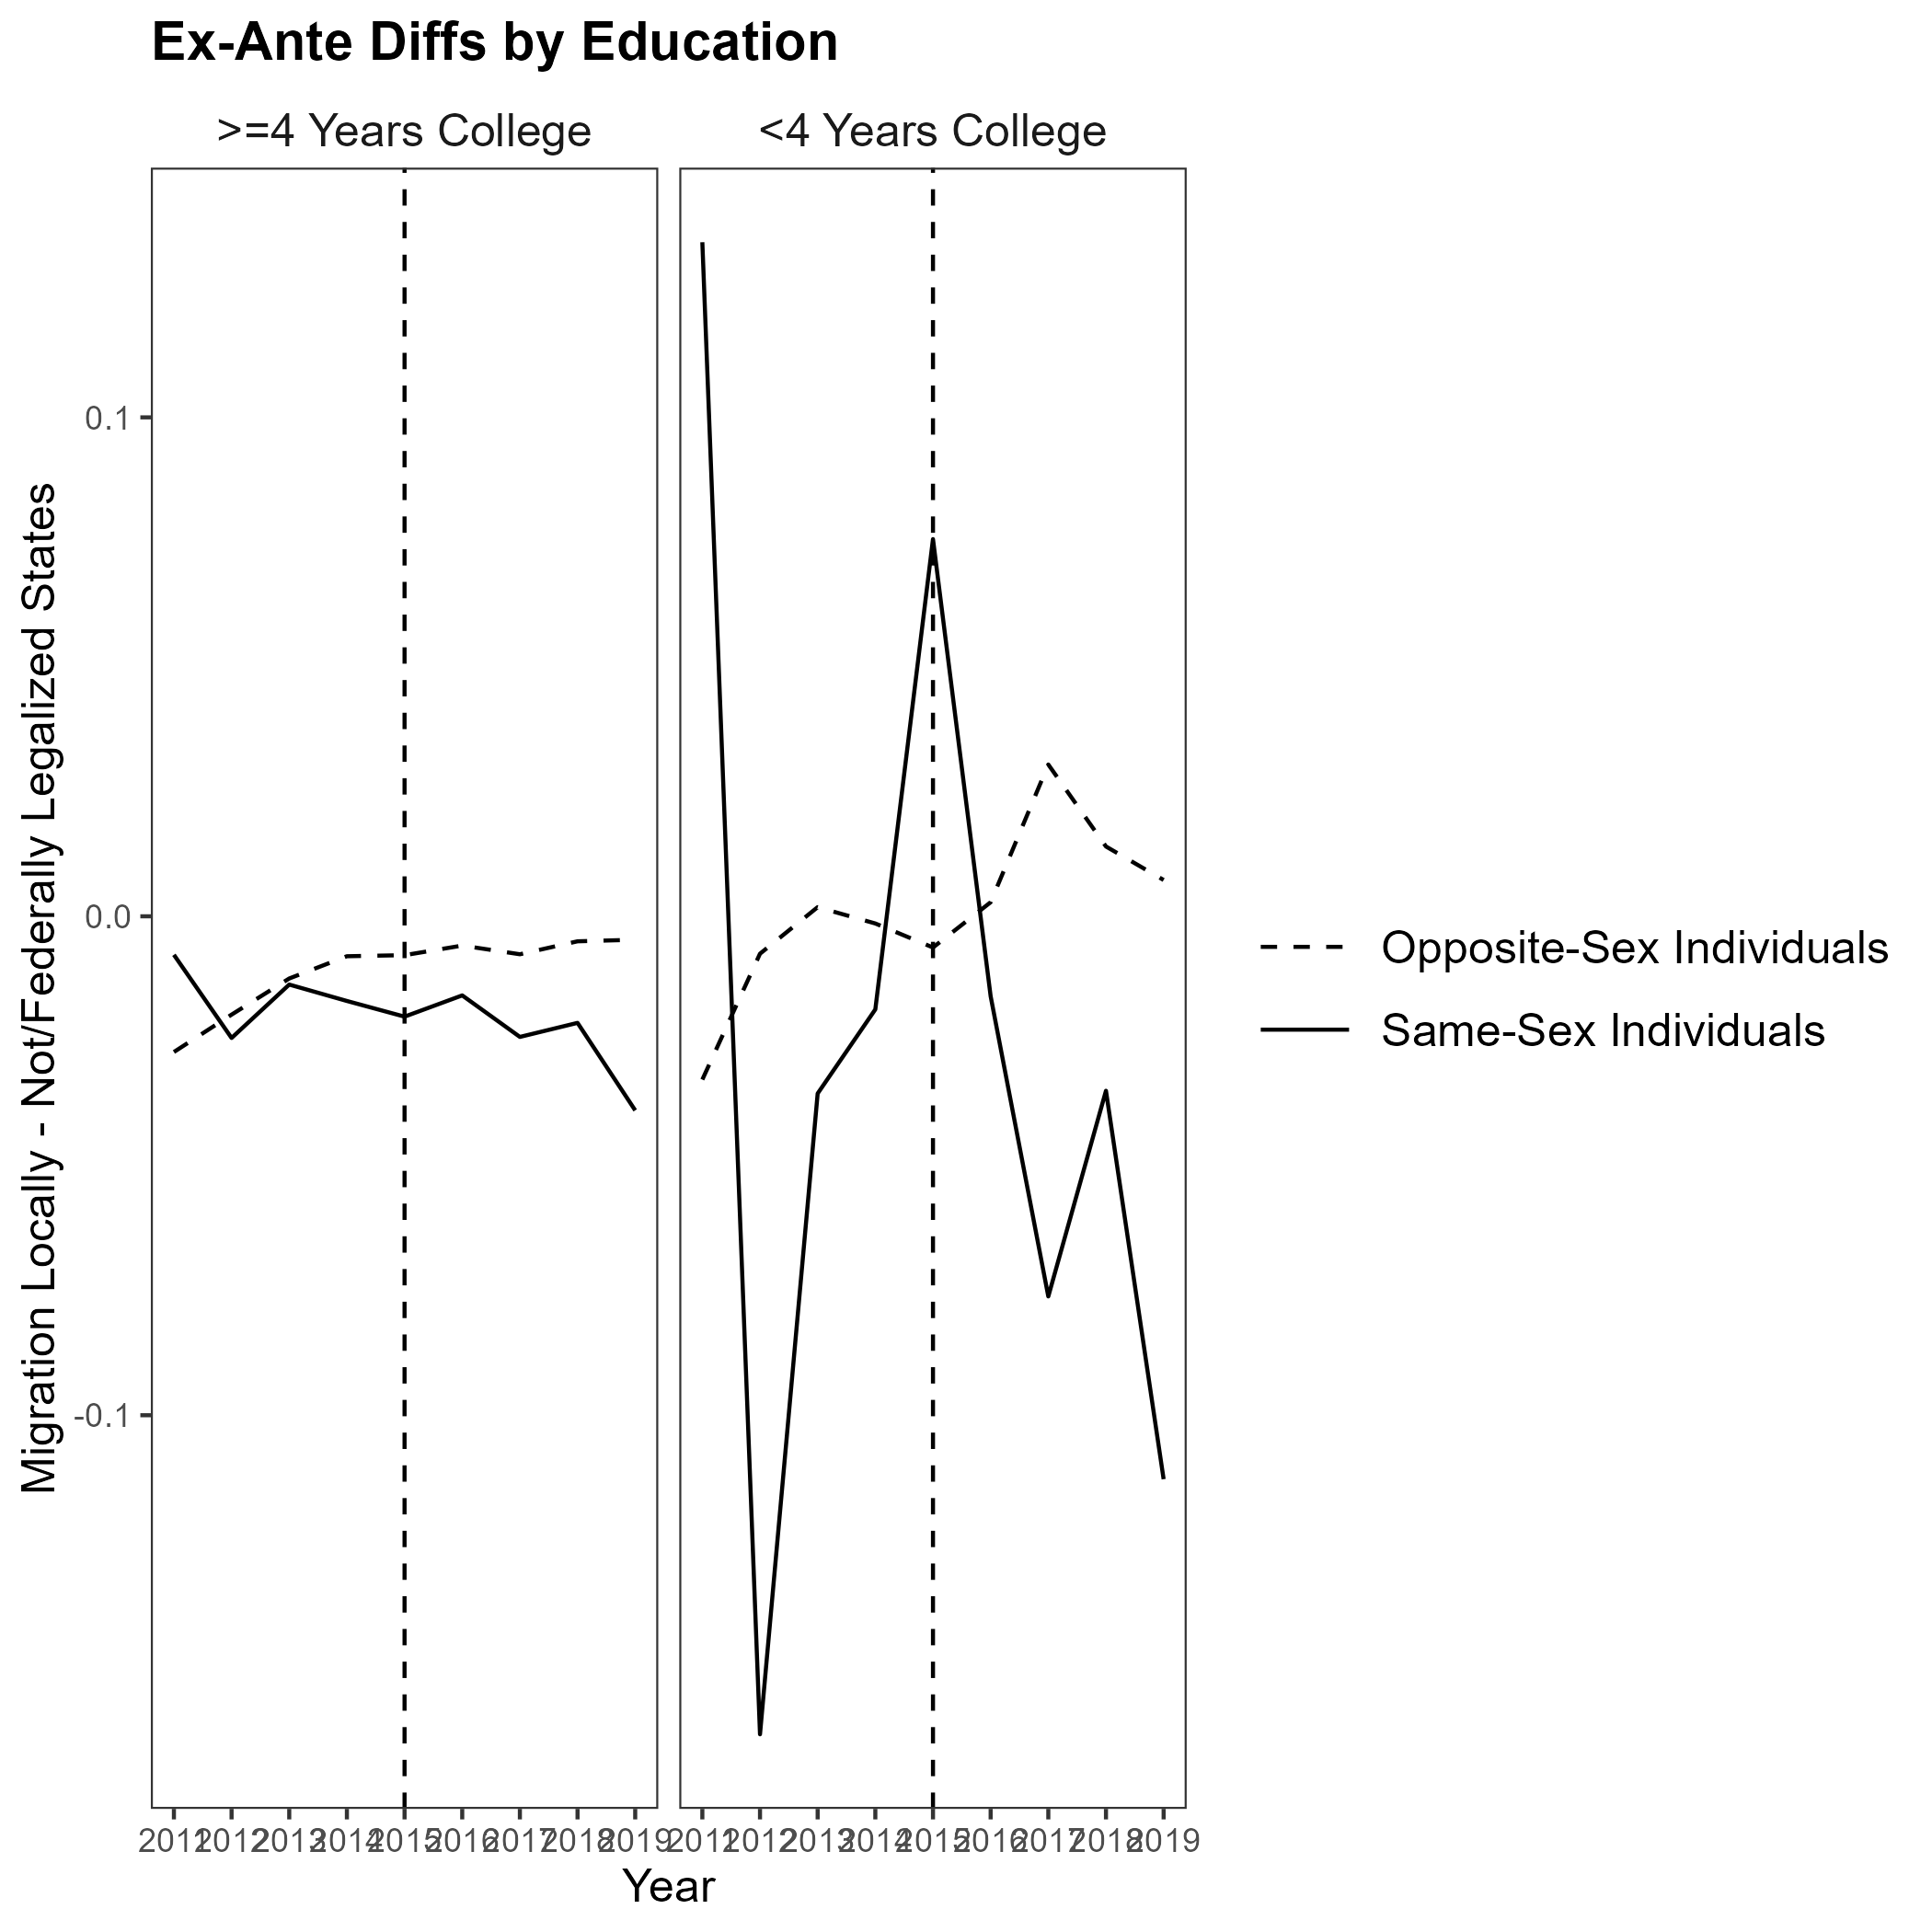
\includegraphics[width=0.75\linewidth]{outputs/summary_stats/educ_ante_diffs.png}
%    \caption{}
%    \label{fig: fig:enter-label}
%\end{figure}

%income
%\begin{figure}[htbp]
%    \centering
%    \includegraphics[width=0.75\linewidth]%{outputs/summary_stats/inc_post_diffs.png}
%    \caption{}
%    \label{fig: fig:enter-label}
%\end{figure}

%\begin{figure}[htbp]
%    \centering
%    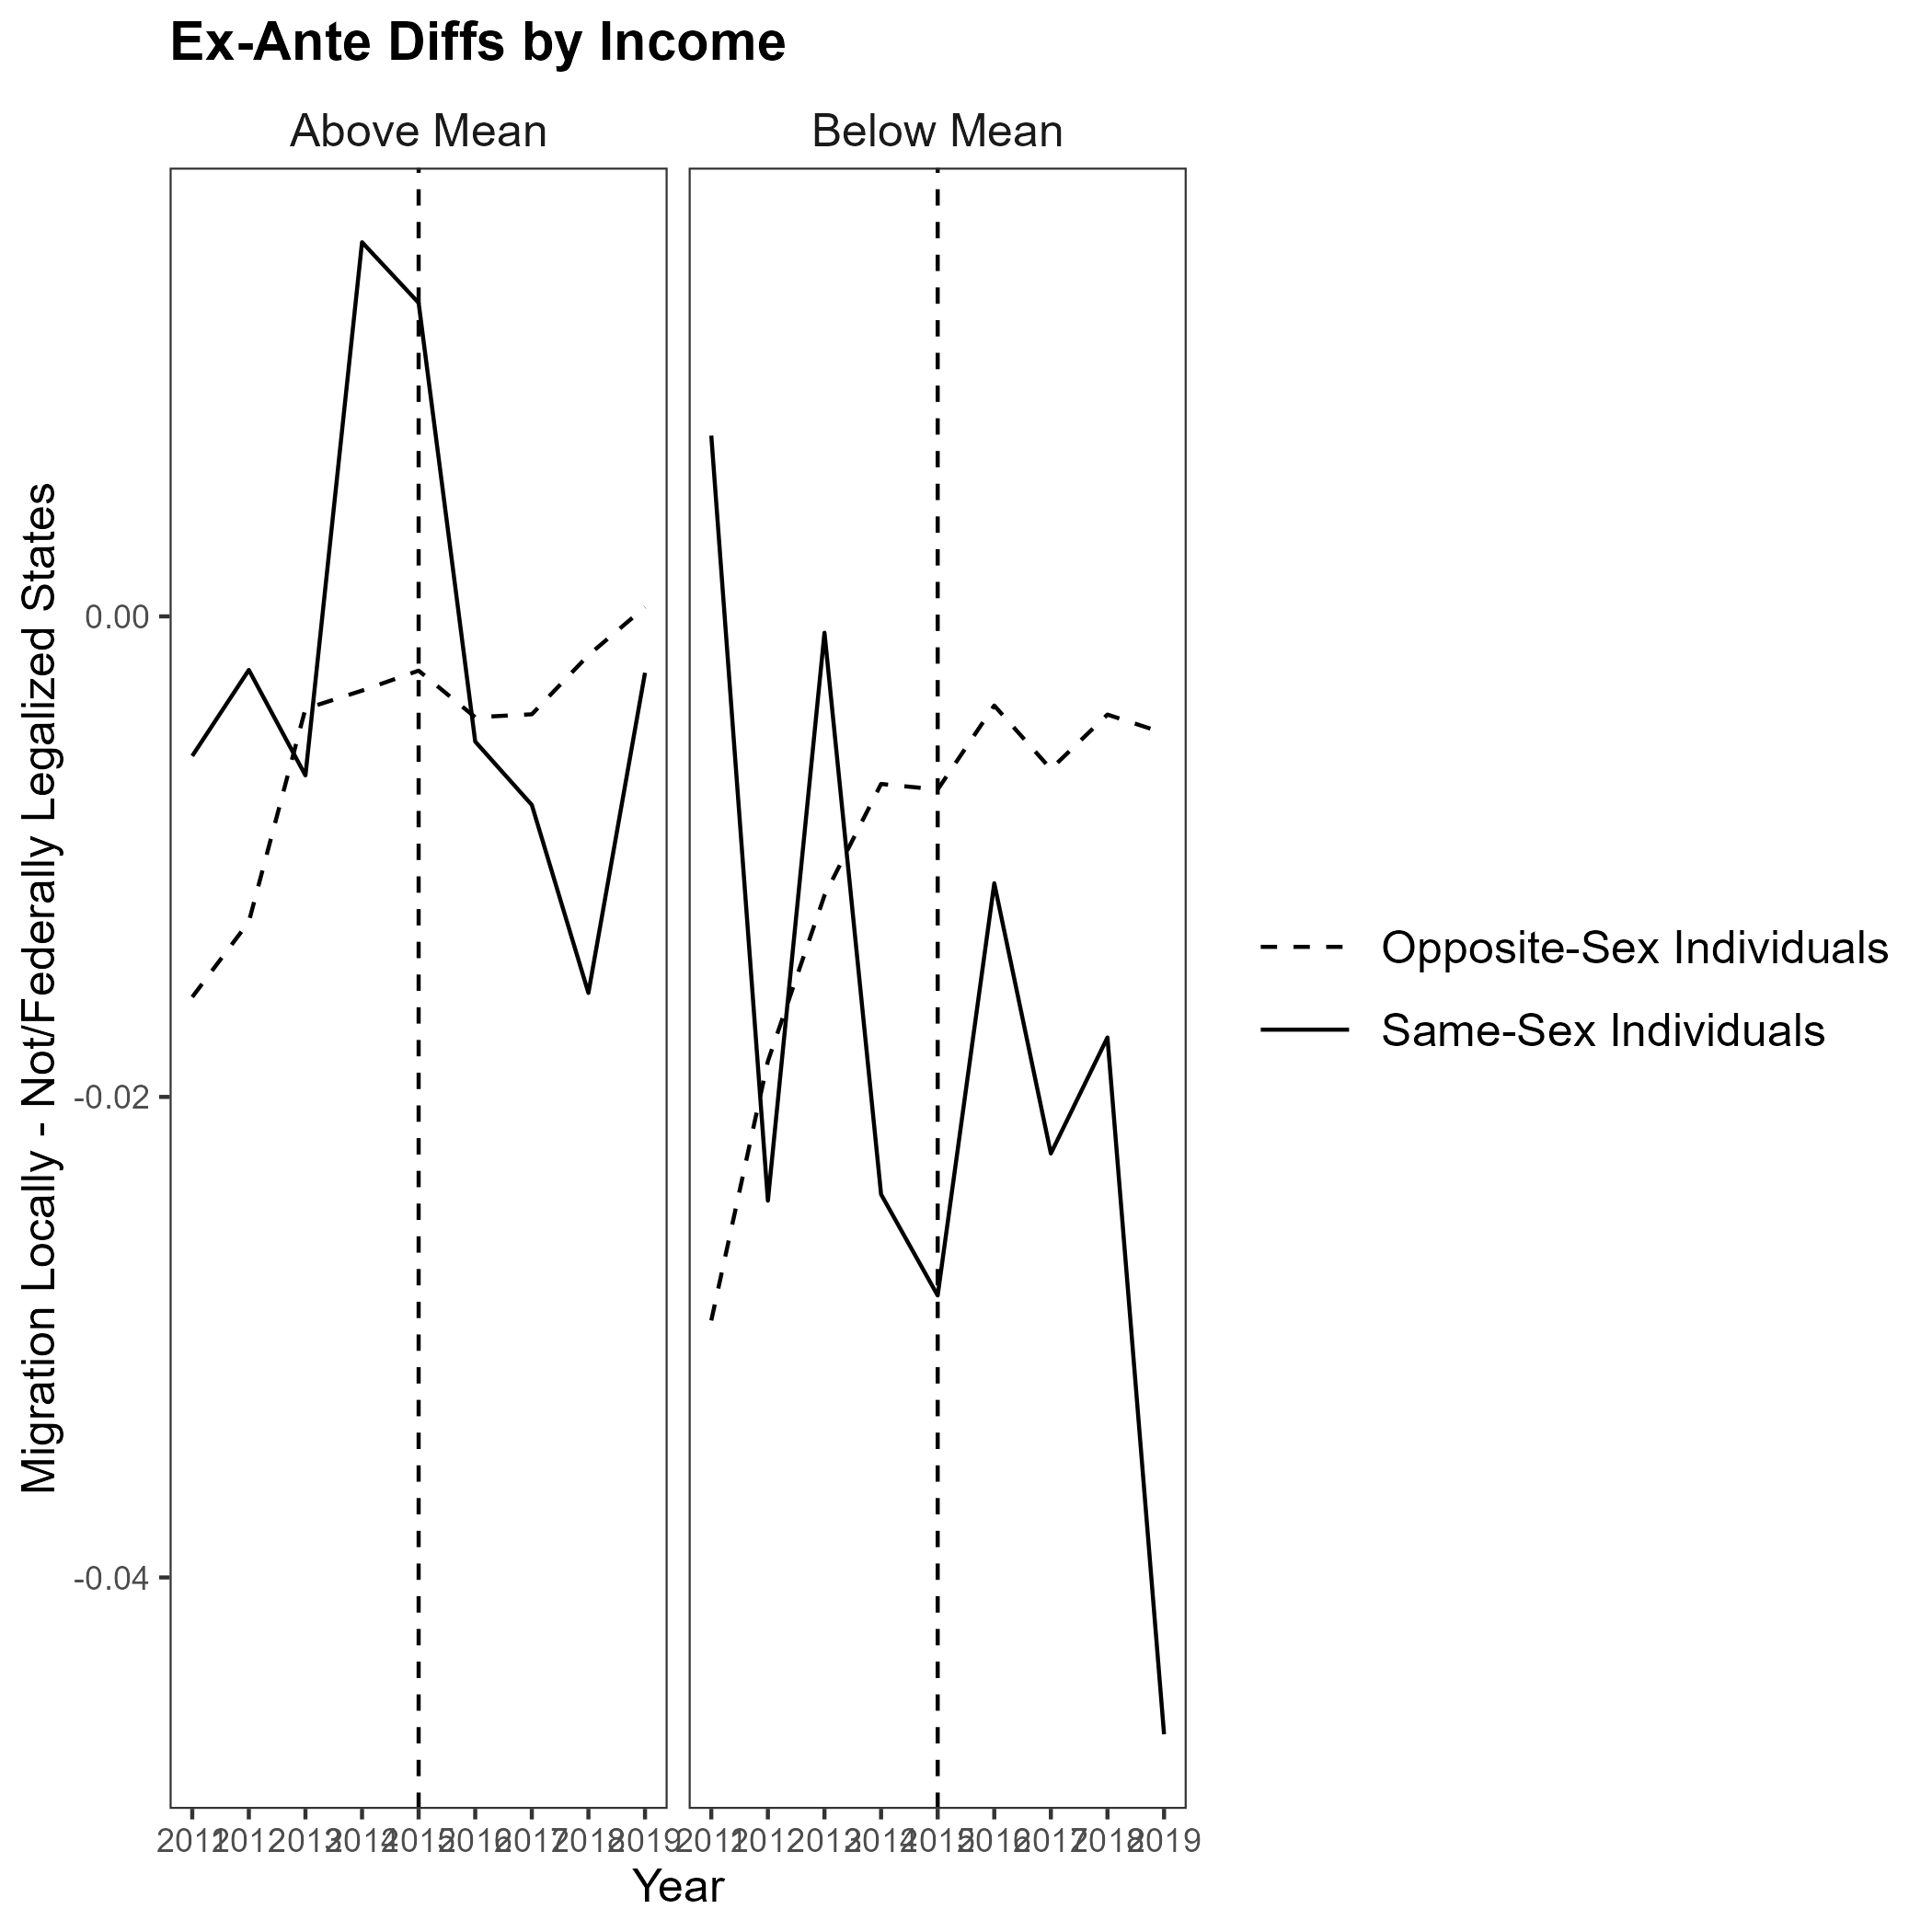
\includegraphics[width=0.75\linewidth]{outputs/summary_stats/inc_ante_diffs.png}
%    \caption{}
%    \label{fig: fig:enter-label}
%\end{figure}

%gender
\begin{figure}[htbp]
    \centering
    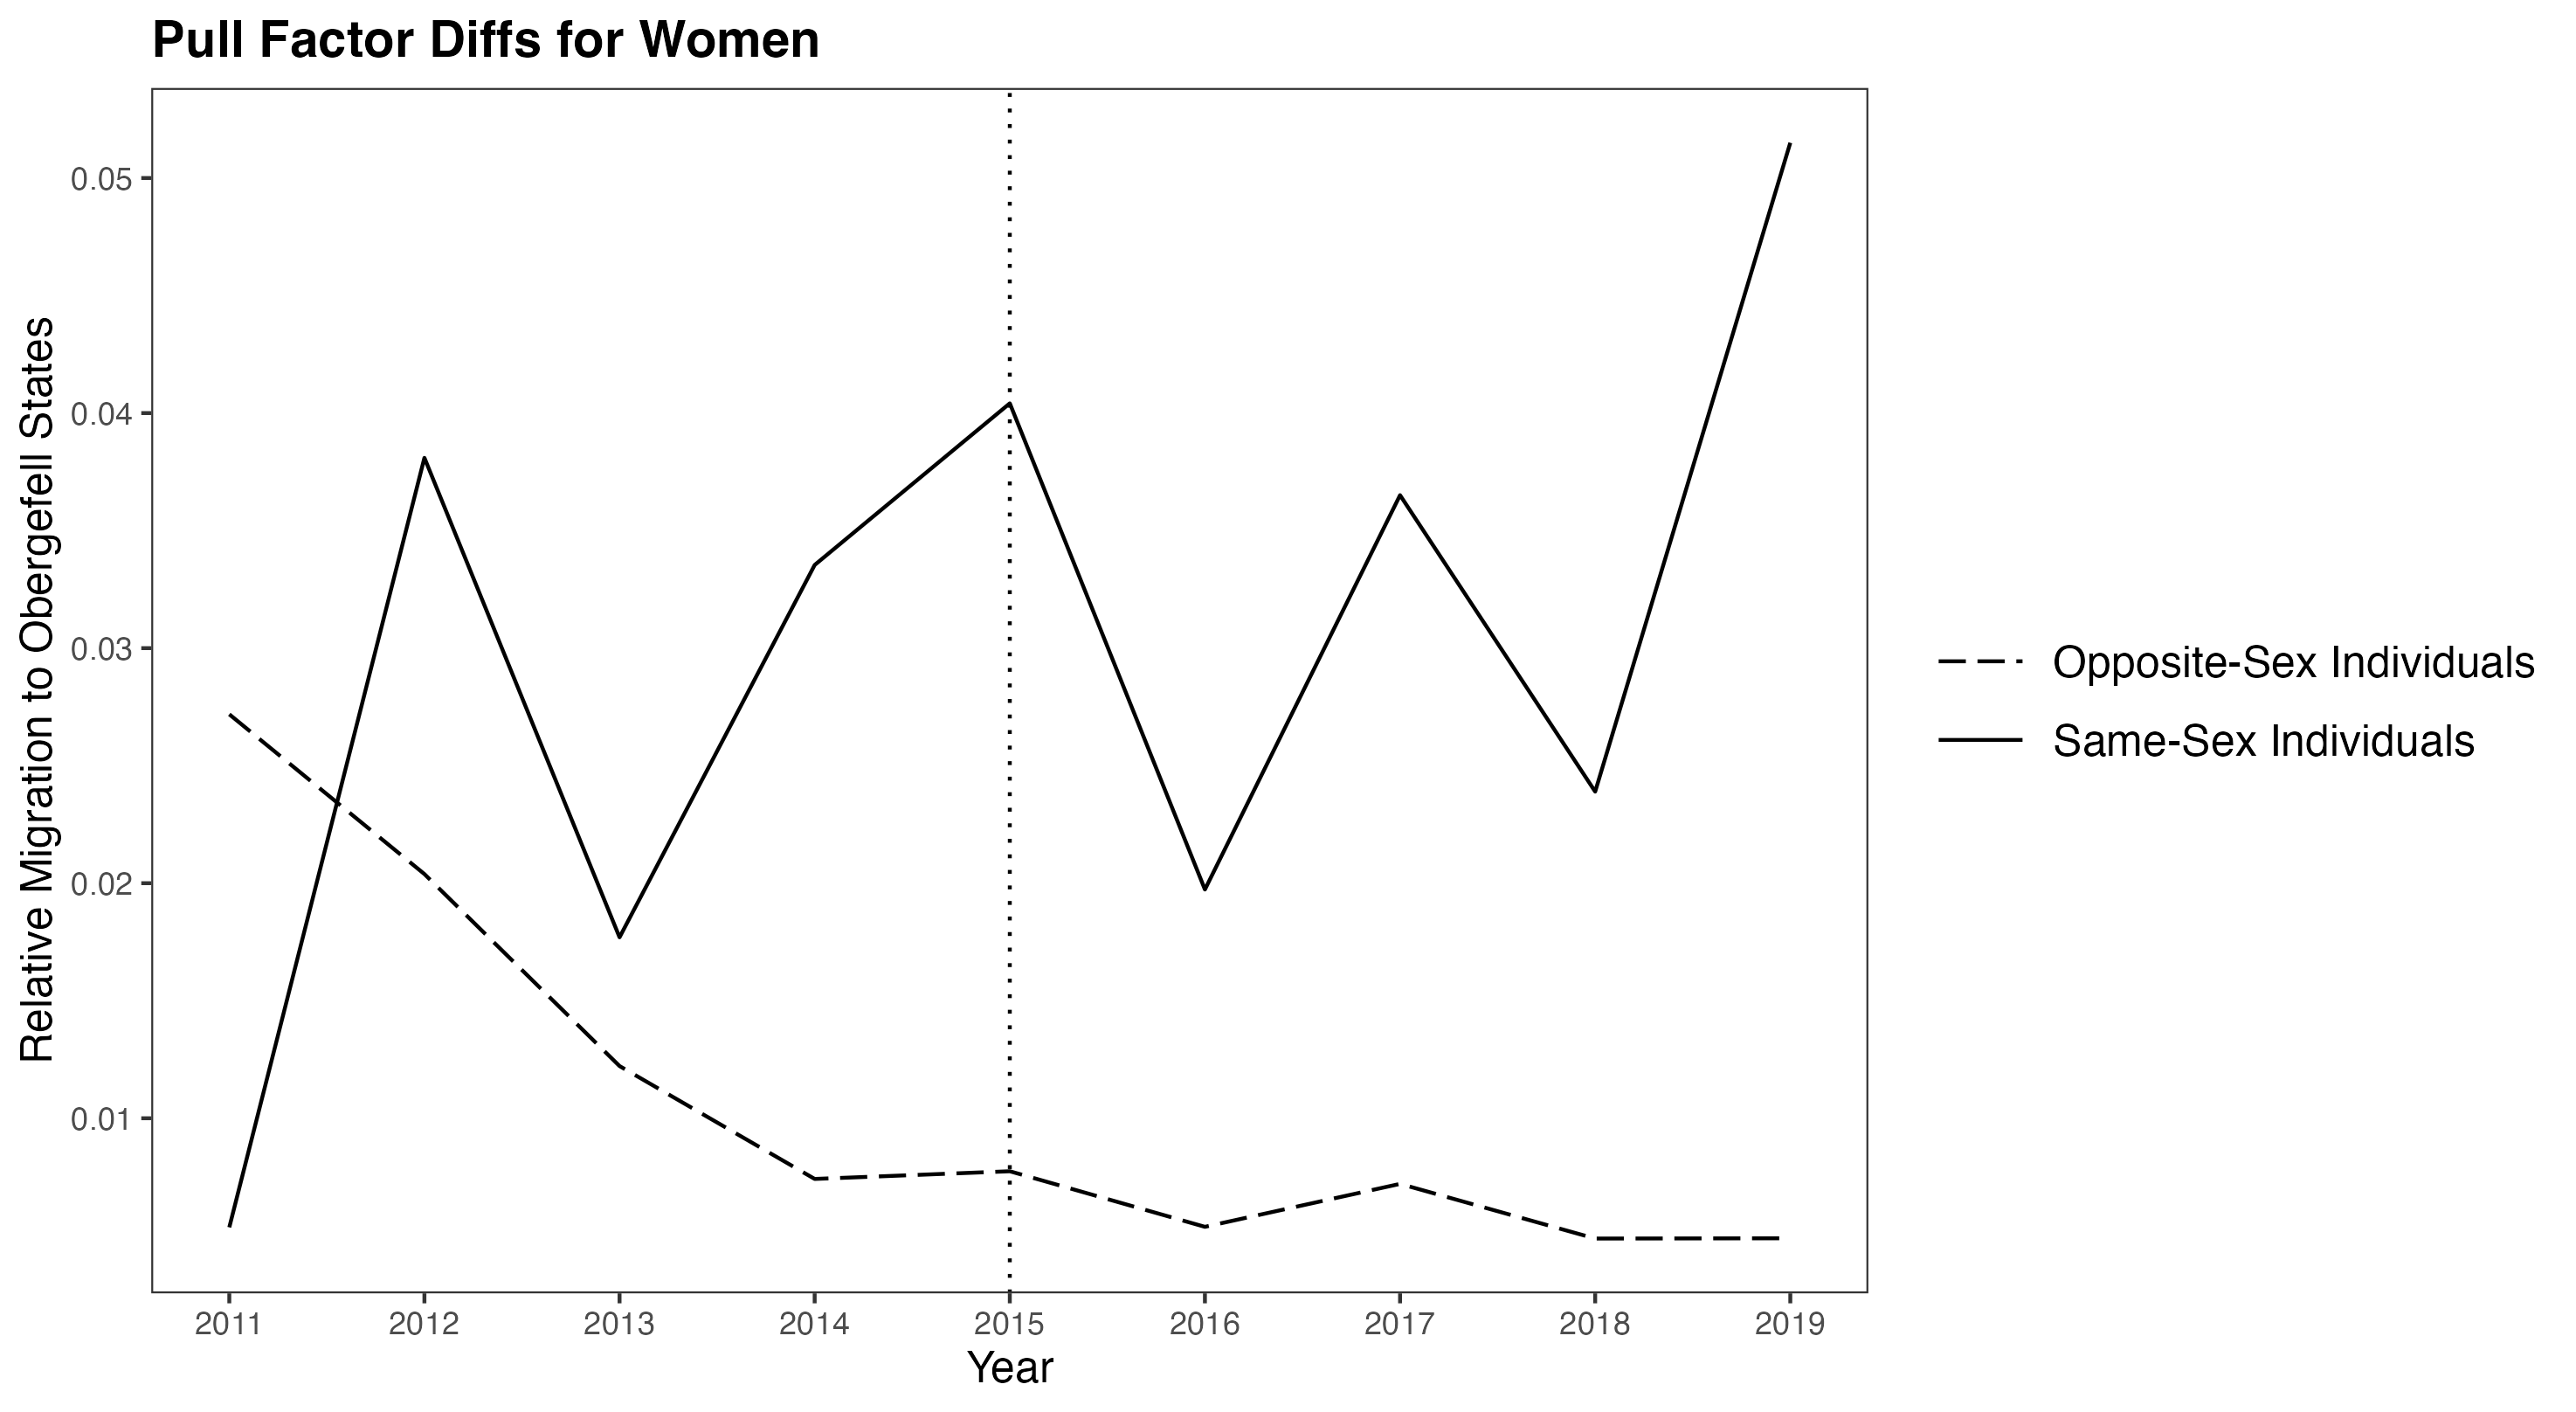
\includegraphics[width=1\linewidth]{outputs/summary_stats/women_post_diffs.png}
    \caption{}
    \label{fig: women_post_diffs}
\end{figure}
\begin{figure}[htbp]
    \centering
    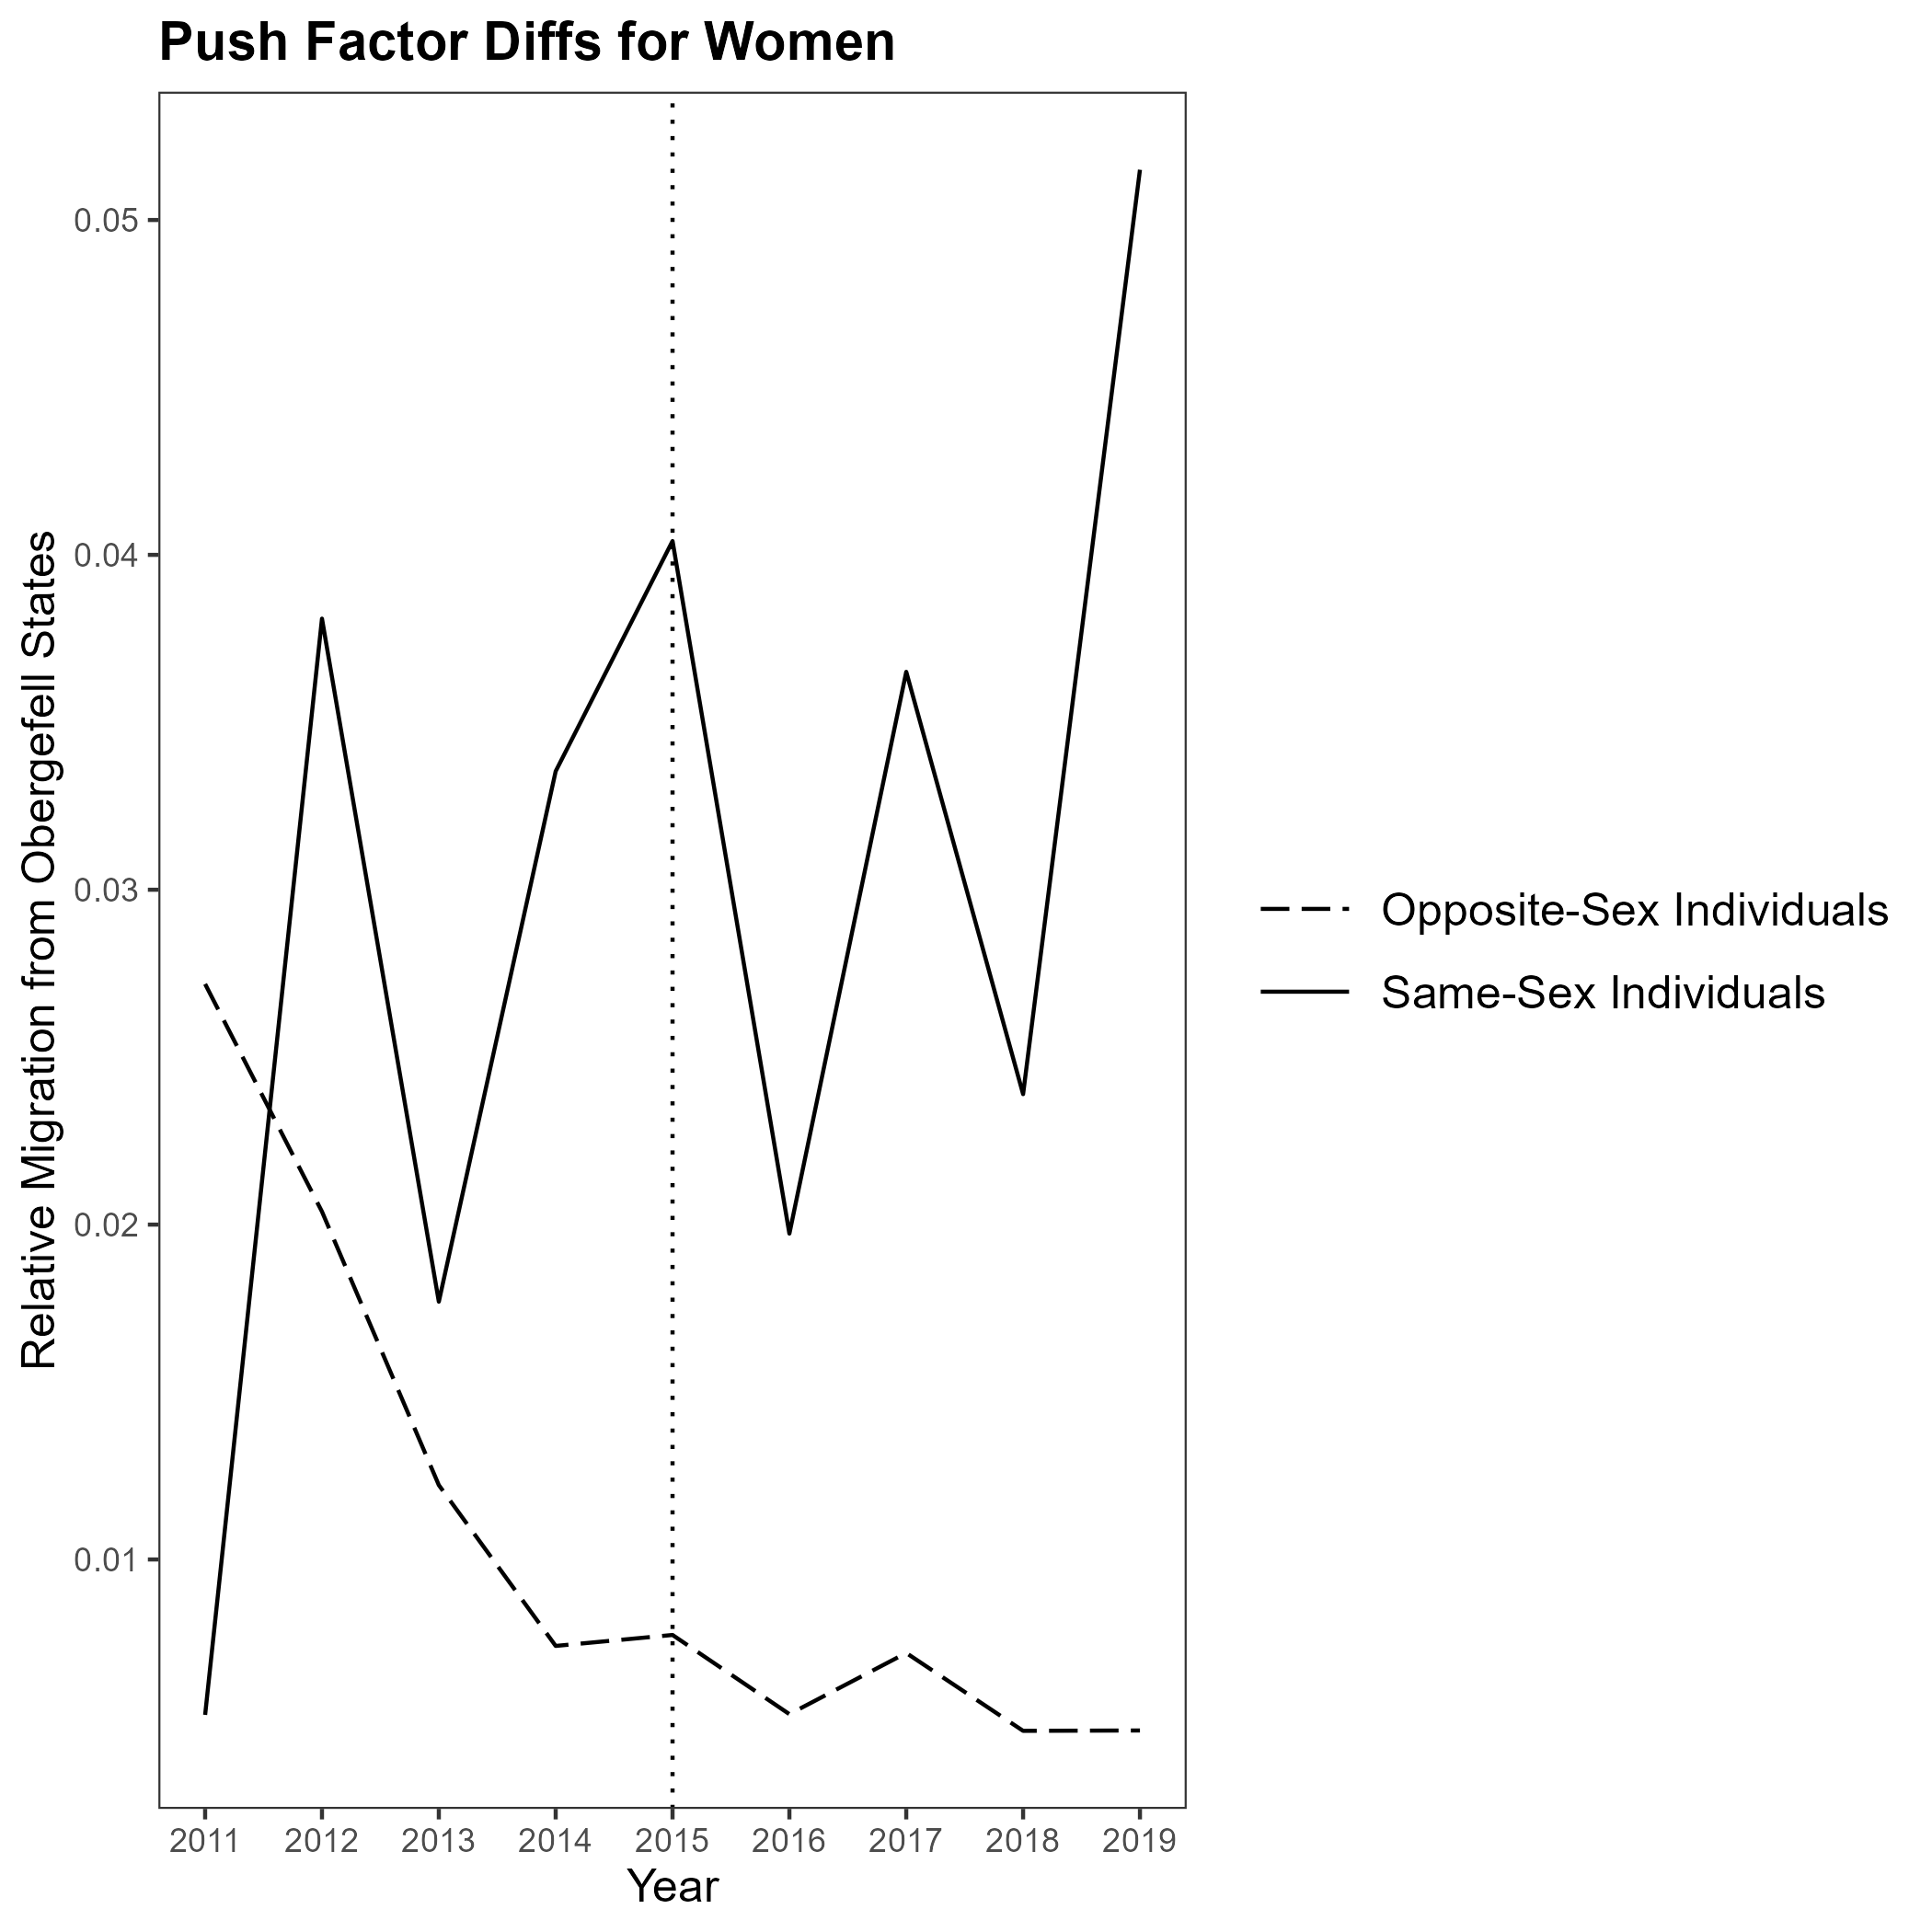
\includegraphics[width=1\linewidth]{outputs/summary_stats/women_ante_diffs.png}
    \caption{}
    \label{fig: women_ante_diffs}
\end{figure}

%region
\begin{figure}[htbp]
    \centering
    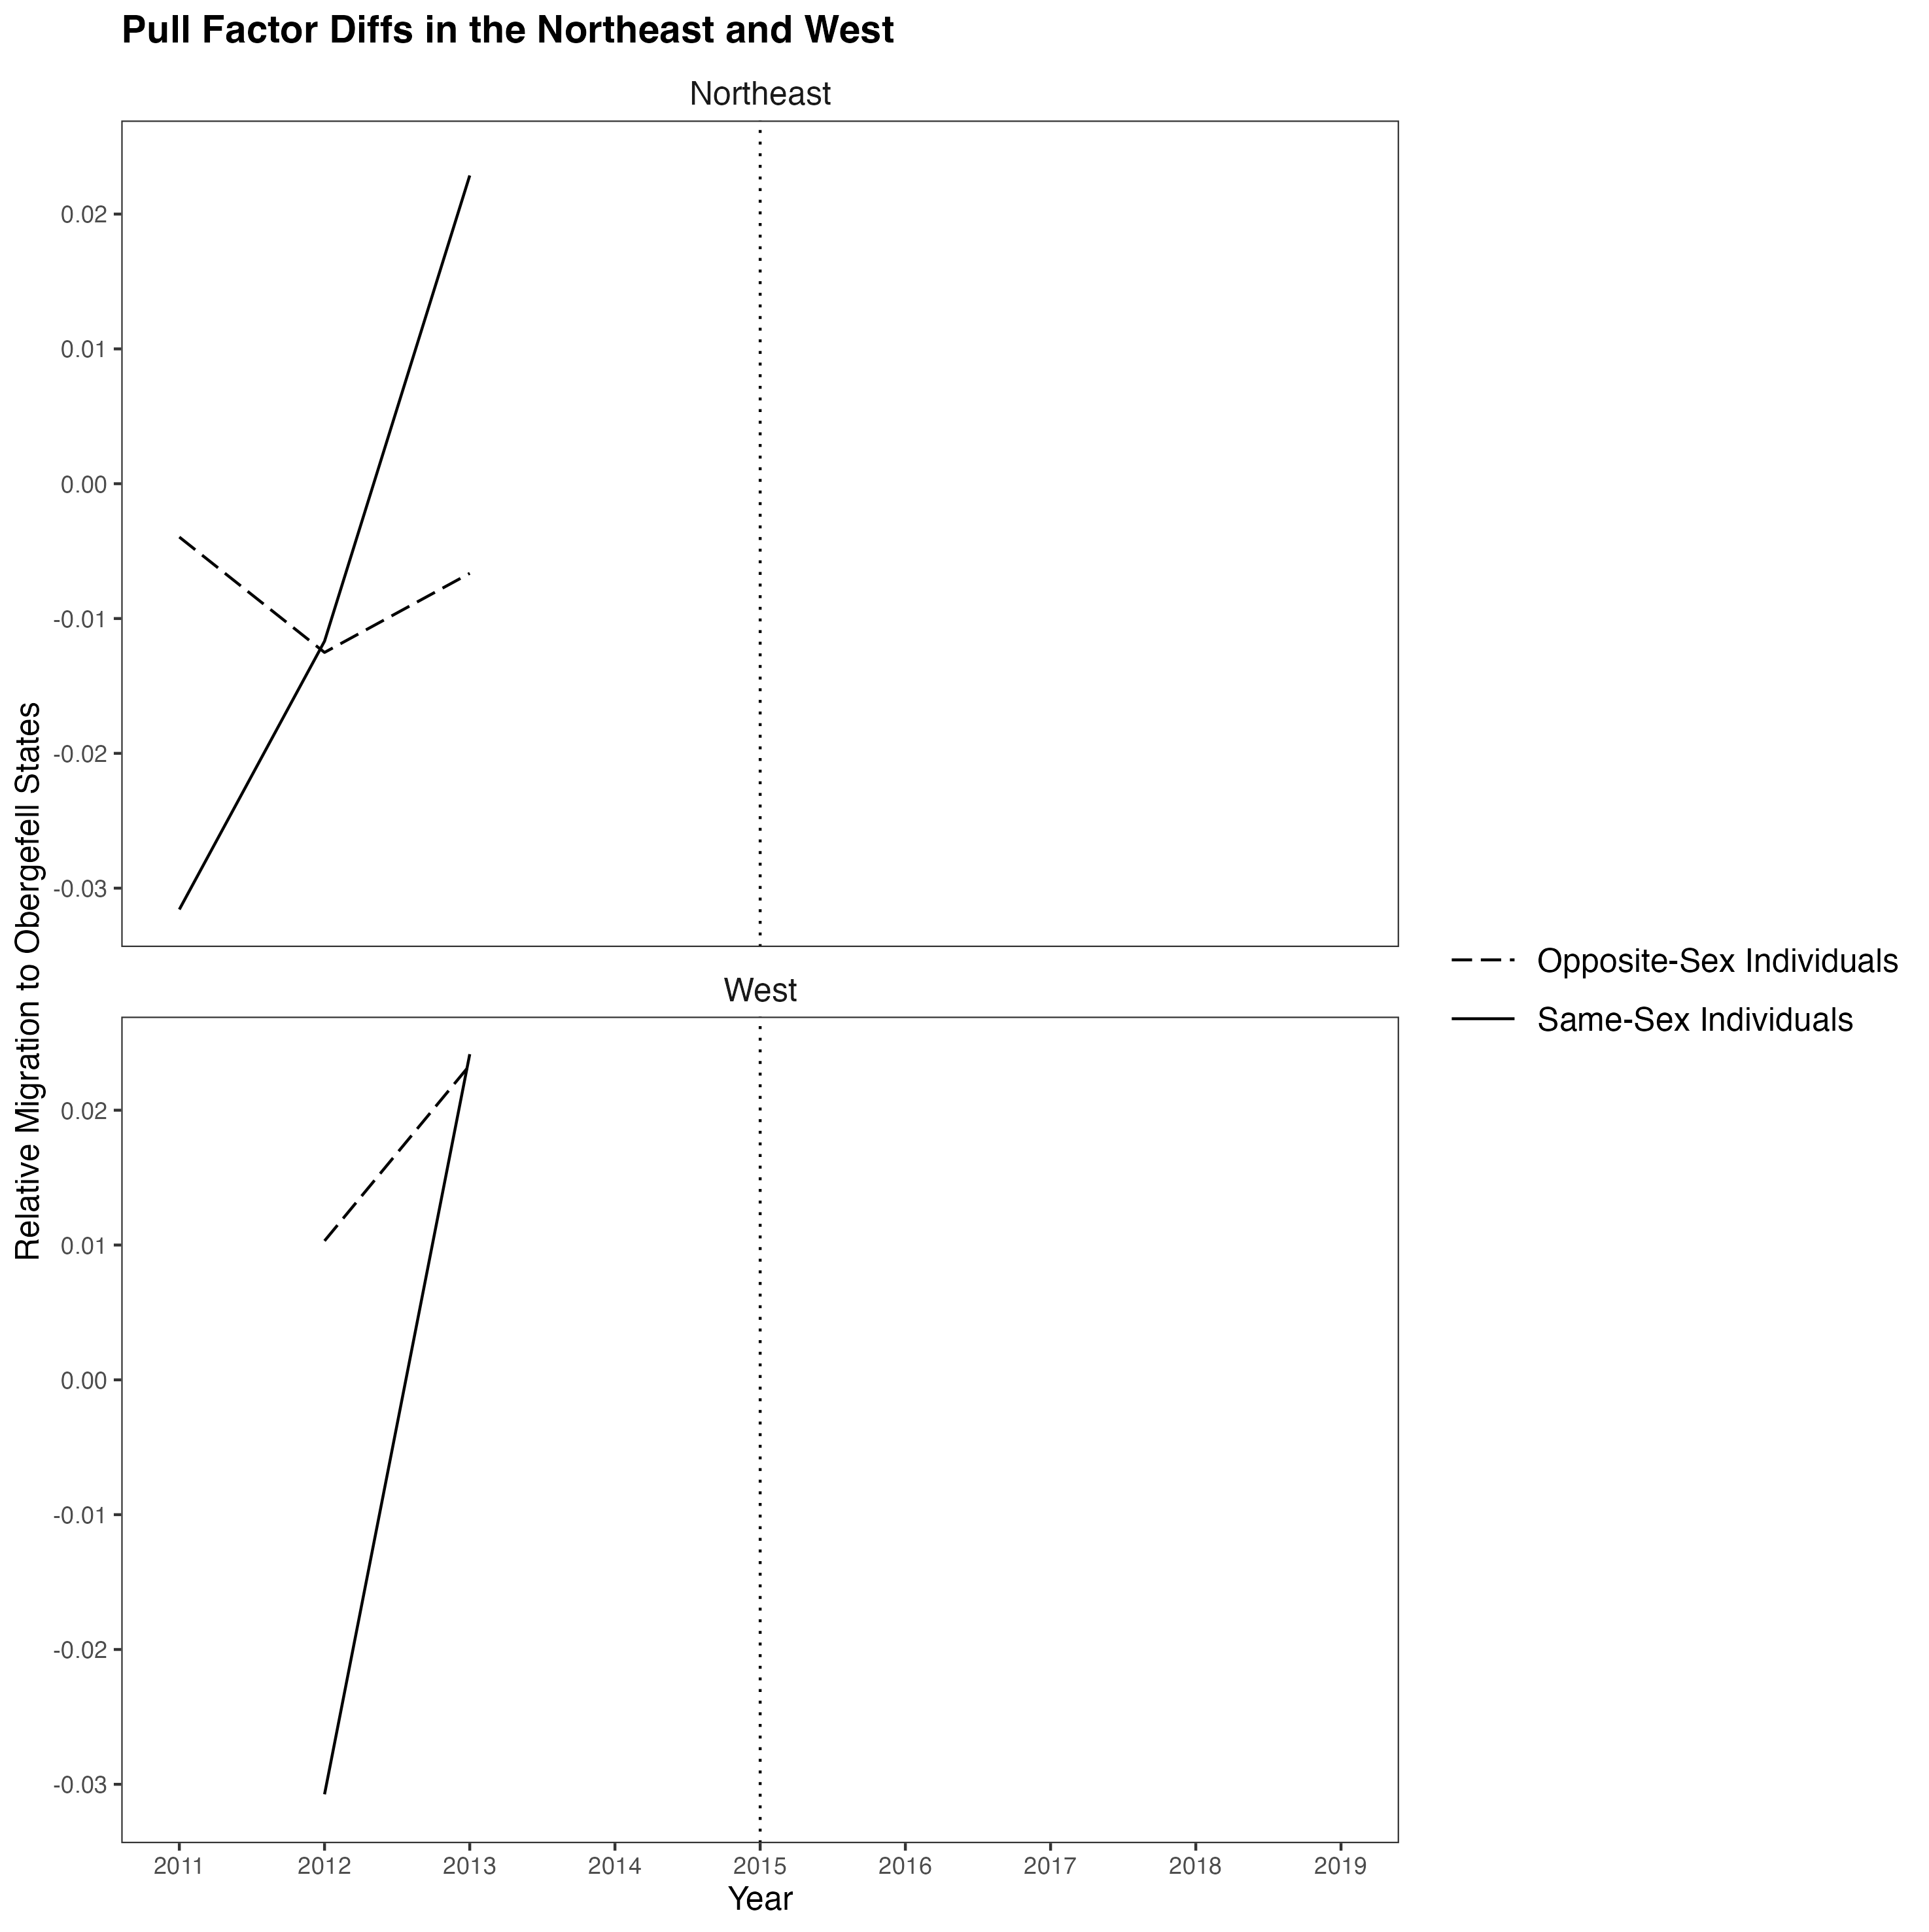
\includegraphics[width=1\linewidth]{outputs/summary_stats/region_post_diffs_app.png}
    \caption{}
    \label{fig: region_post_diffs_app}
\end{figure}

\begin{figure}[htbp]
    \centering
    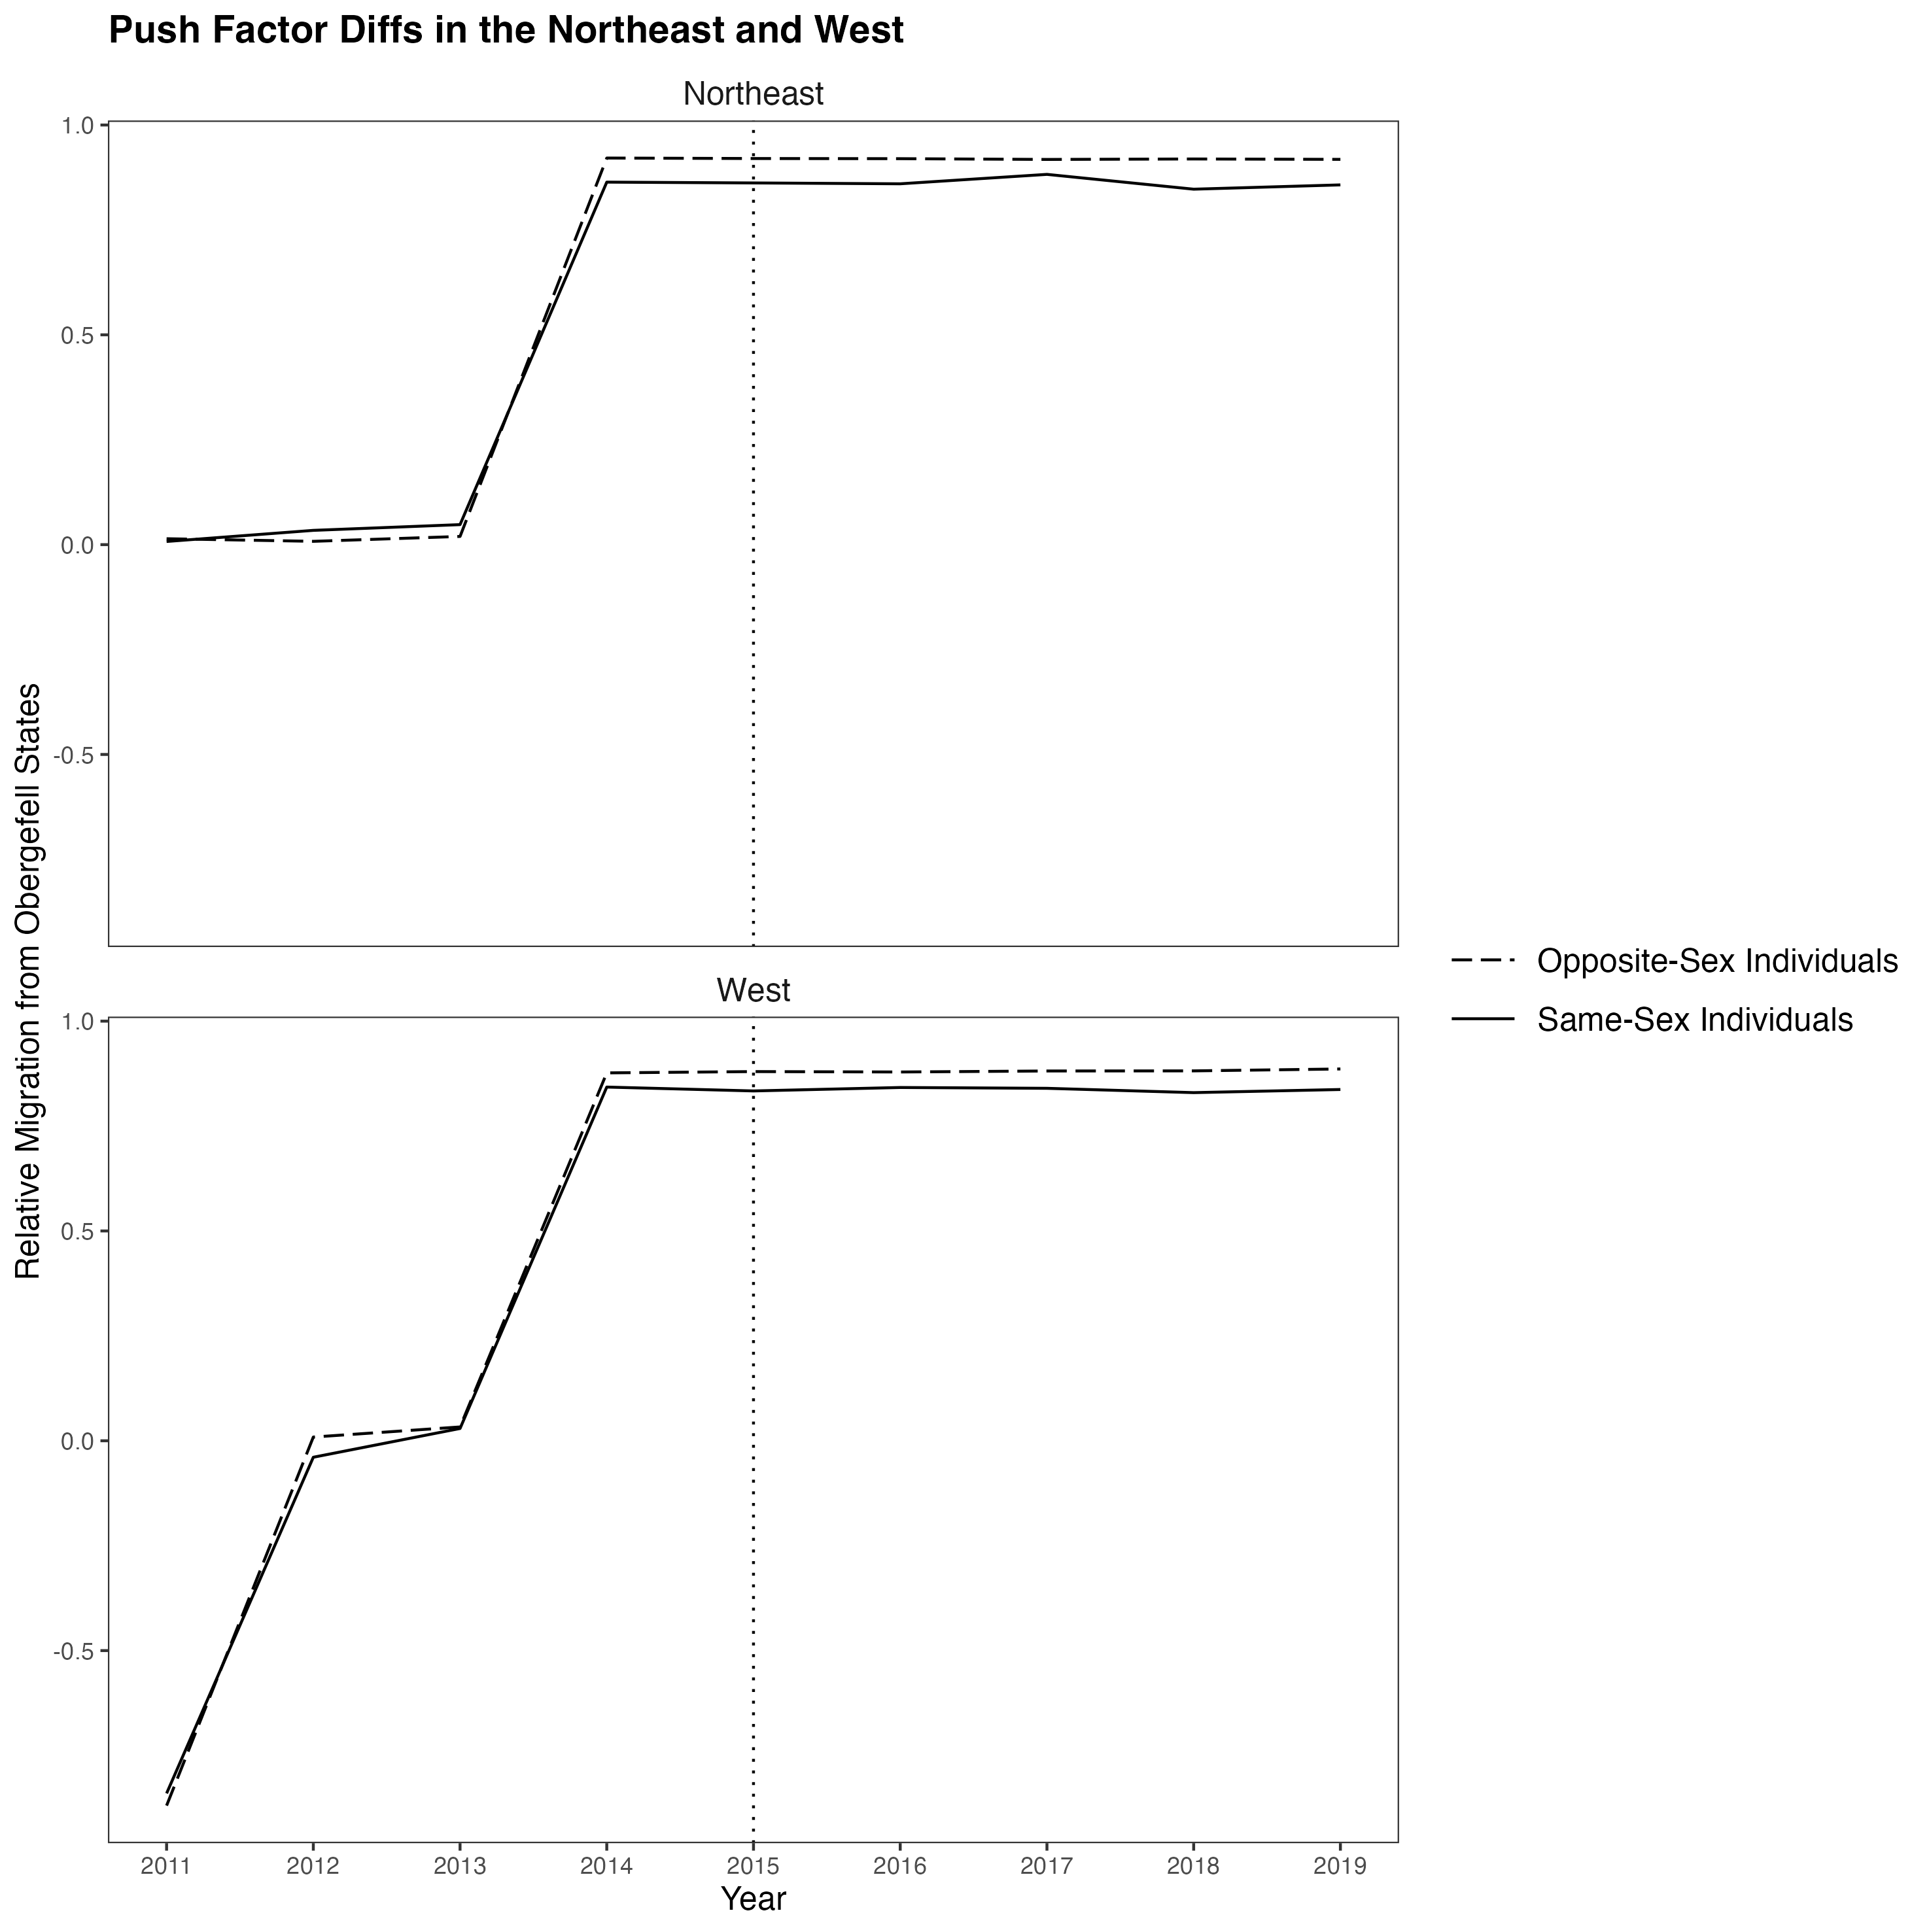
\includegraphics[width=1\linewidth]{outputs/summary_stats/region_ante_diffs_app.png}
    \caption{}
    \label{fig: region_ante_diffs_app}
\end{figure}

%flow
\begin{figure}[htbp]
    \centering
    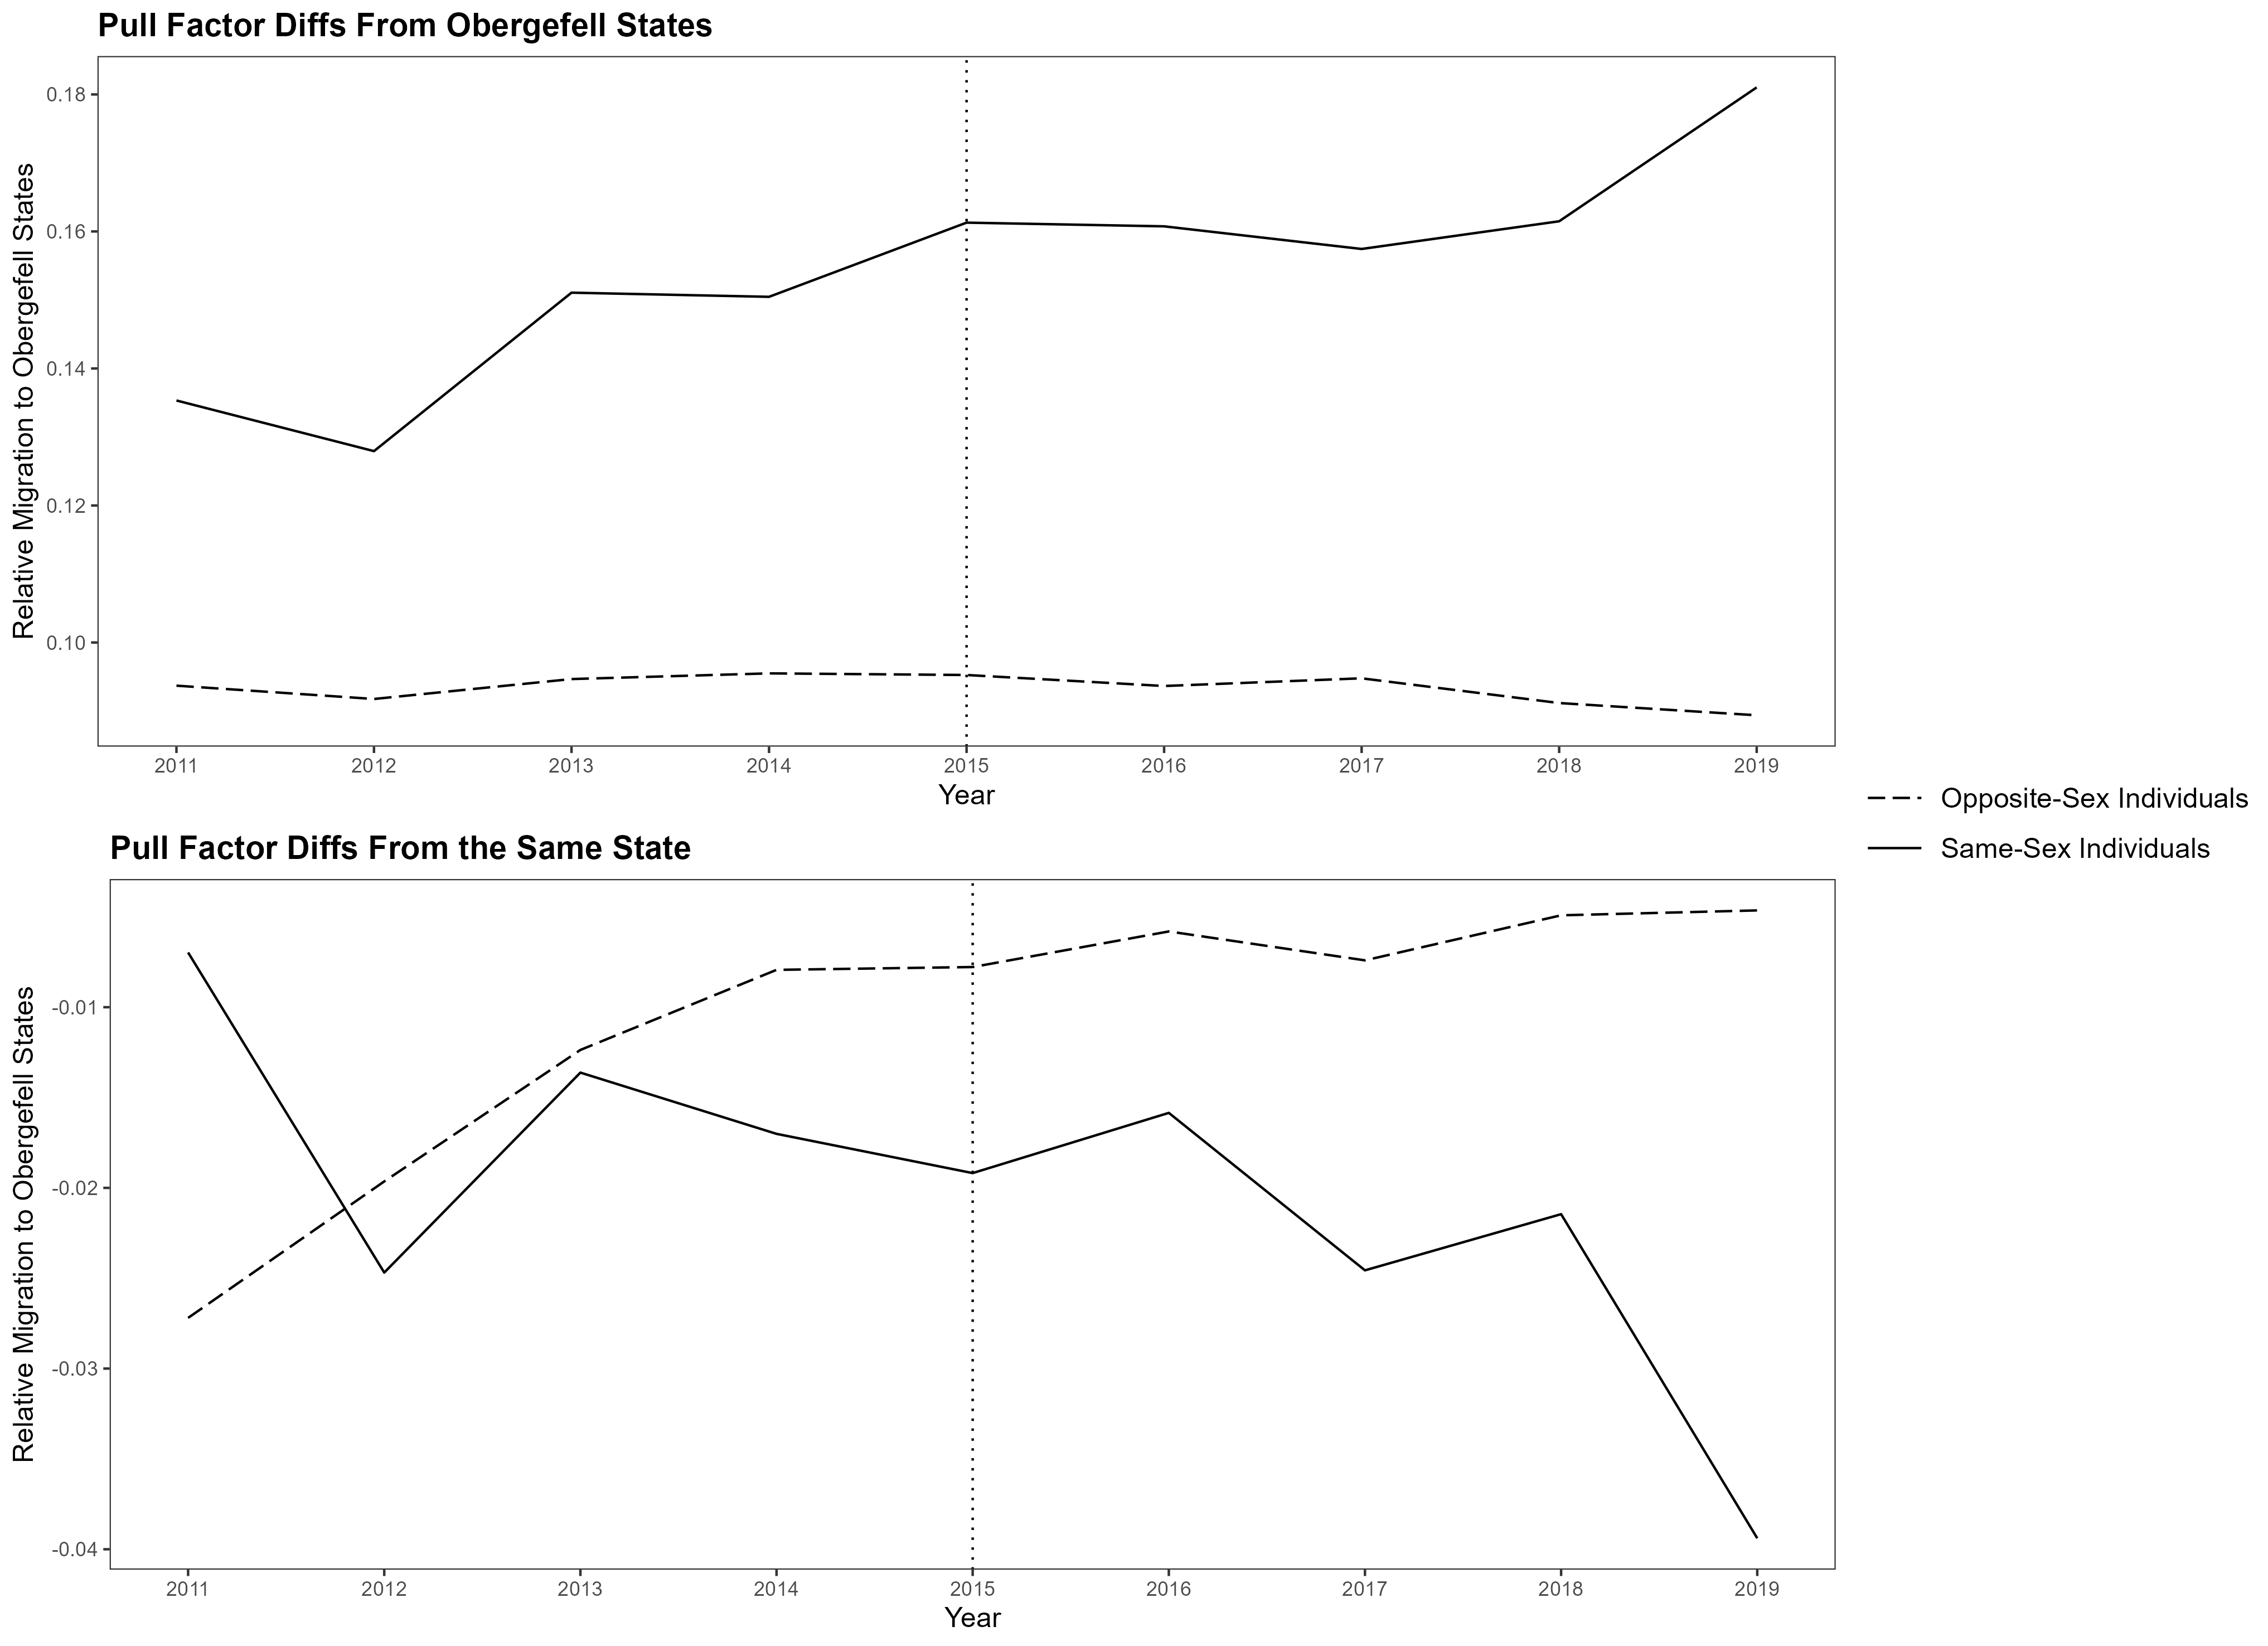
\includegraphics[width=1\linewidth]{outputs/summary_stats/flows_post_diffs_app.png}
    \caption{}
    \label{fig: flows_post_diffs_app}
\end{figure}
\begin{figure}[htbp]
    \centering
    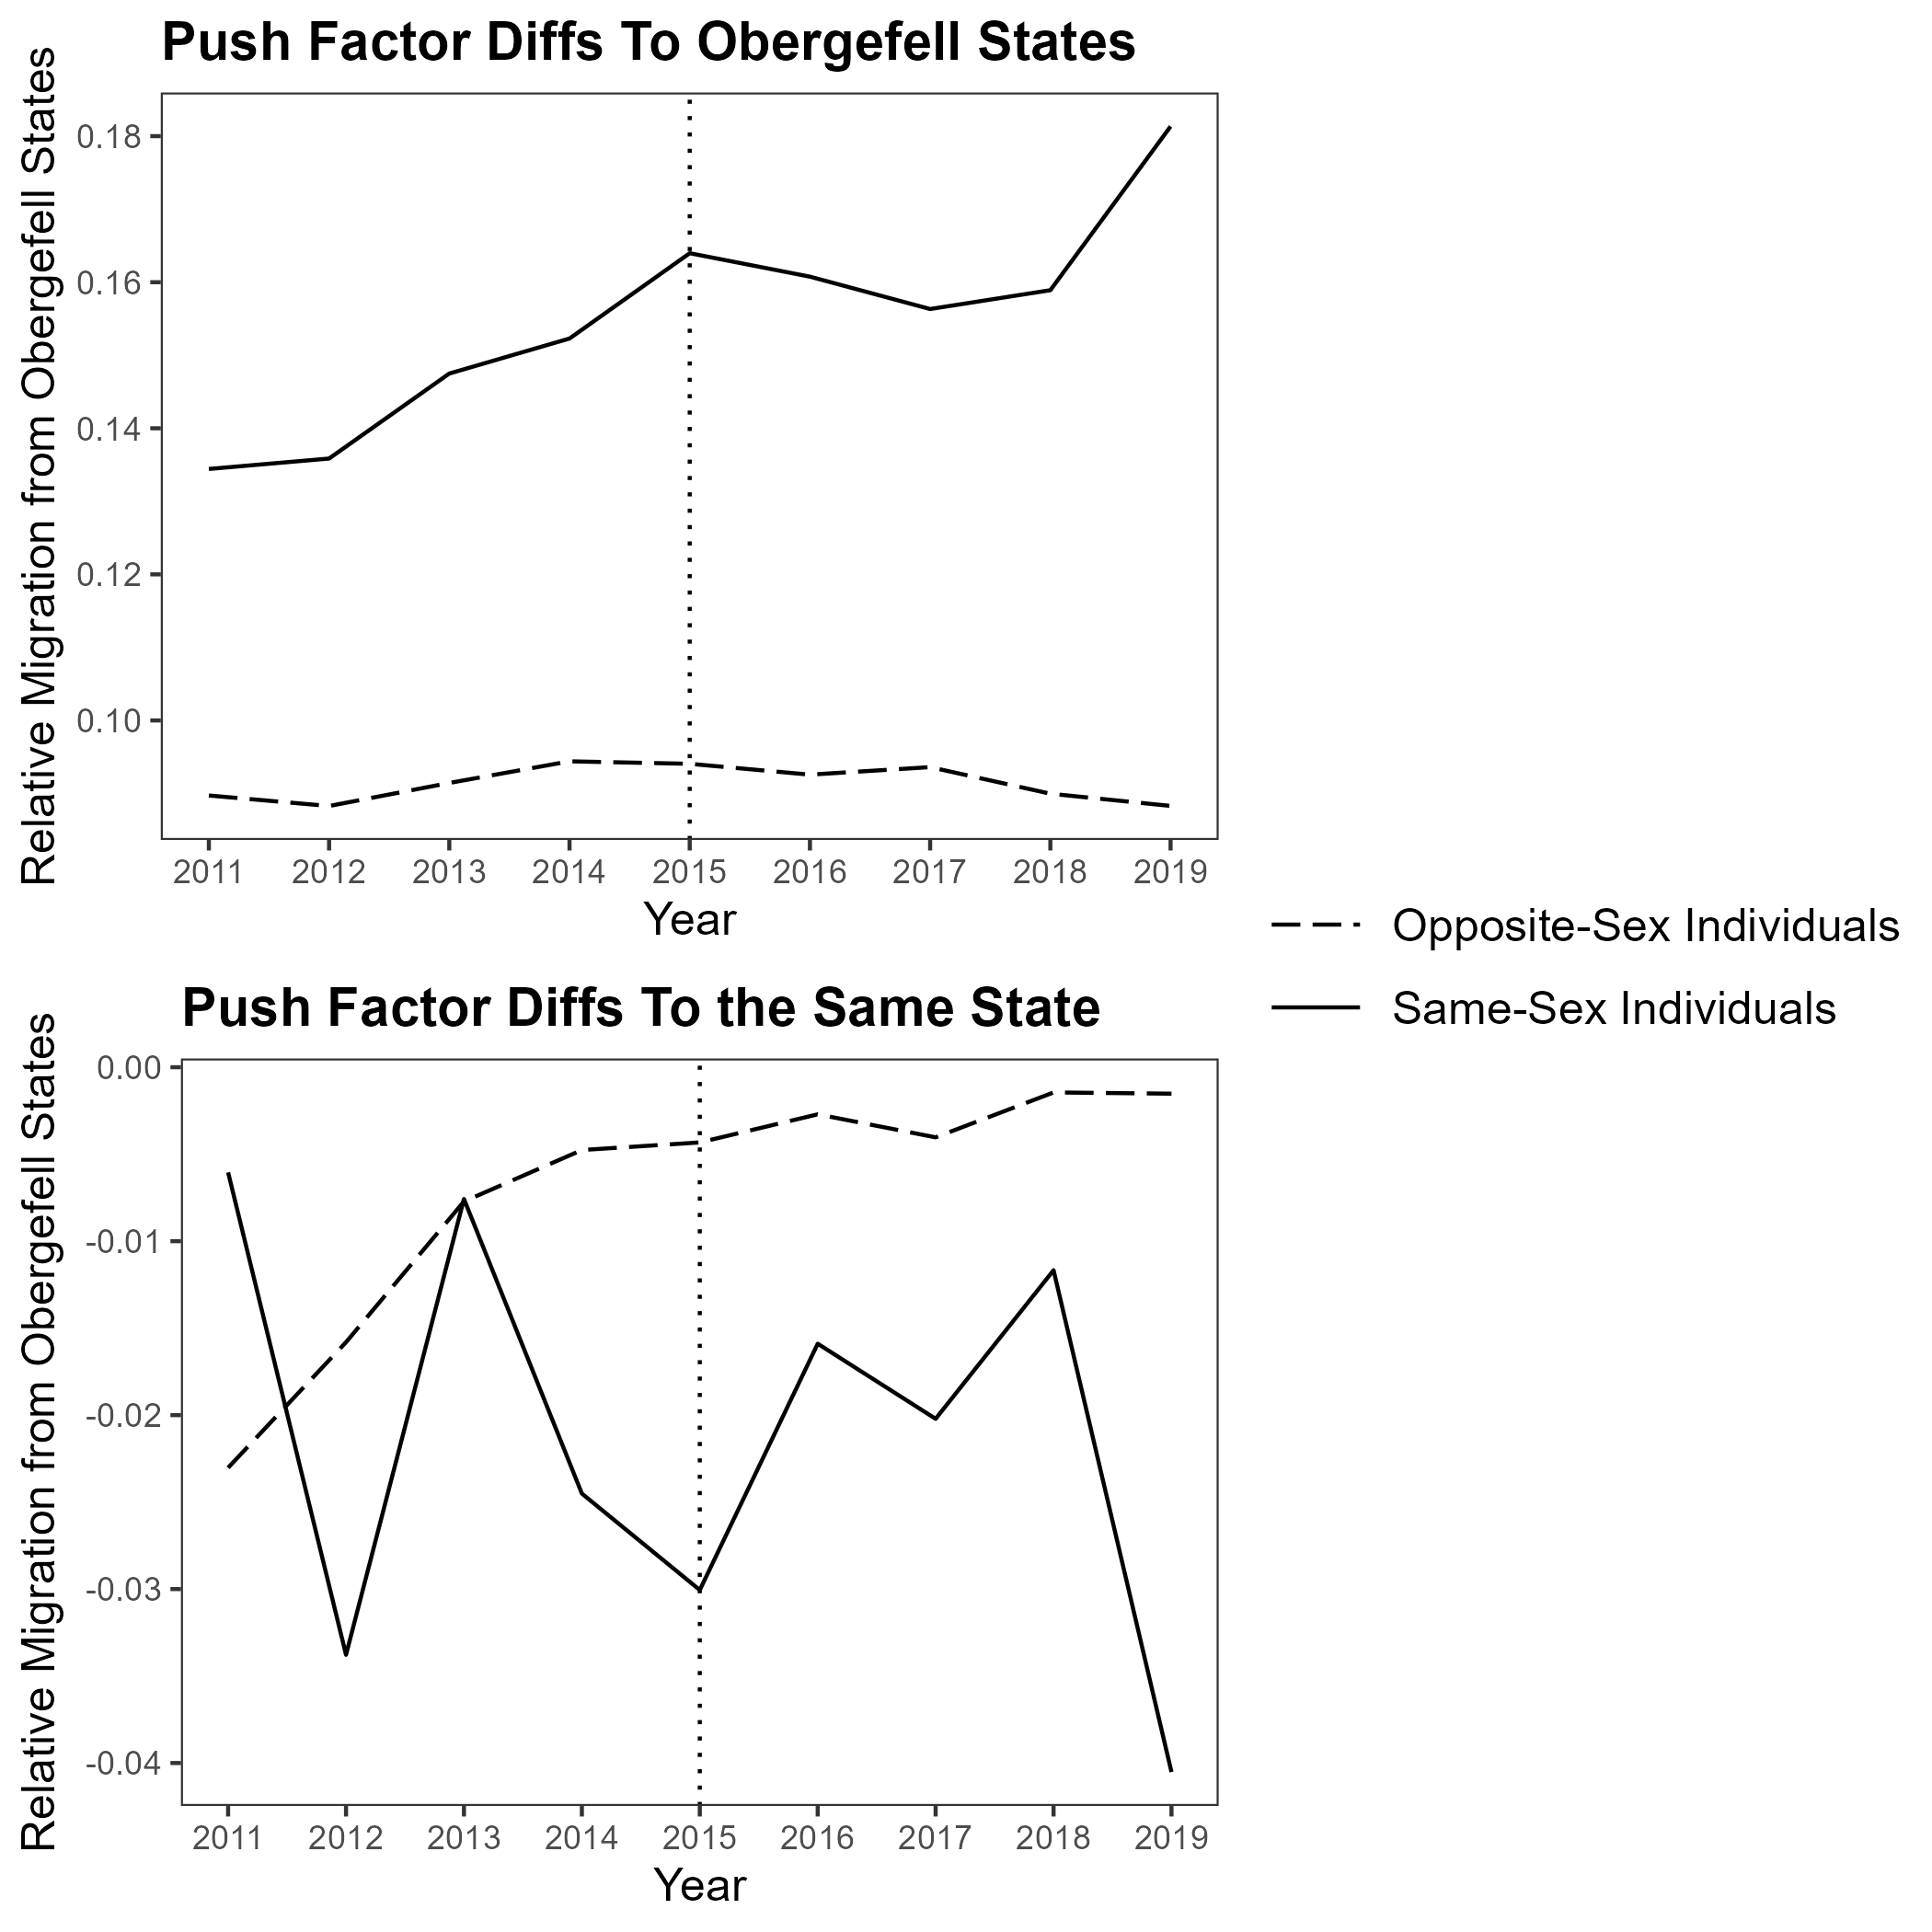
\includegraphics[width=1\linewidth]{outputs/summary_stats/flows_ante_diffs_app.png}
    \caption{}
    \label{fig: flows_ante_diffs_app}
\end{figure}

%regression tables
\FloatBarrier
\newpage
\section{Additional Regression Tables}
%additional sex tables
\begin{table}[htbp]
    \centering
    \caption{Pull Factor Model: Female}
    \label{tab: female_expost_model}
    \begin{tabular}{lccc}
\hline
 & (1) & (2) & (3) \\
VARIABLES & Model 1 & Model 2 & Model 3 \\ \hline
 &  &  &  \\
$\hat{\beta_1}$ & 0.006 & -0.007 & -0.008 \\
 & (0.012) & (0.030) & (0.033) \\
Constant & 0.104*** & 3.856*** & 3.753*** \\
 & (0.000) & (0.102) & (0.098) \\
 &  &  &  \\
Observations & 17,942 & 17,942 & 17,942 \\
 R-squared & 0.005 & 0.916 & 0.920 \\ \hline
\multicolumn{4}{c}{ Robust standard errors in parentheses} \\
\multicolumn{4}{c}{ *** p$<$0.01, ** p$<$0.05, * p$<$0.1} \\
\multicolumn{4}{p{0.8\linewidth}}{\small Column 1 reports the regression coefficient of a model with state, year, and relationship-type fixed effects including corresponding interactions; column 2 reports the regression coefficient of a model with these fixed effects and controls for sex, race, education level, the presence of children in the household, income level, and age; and column 3 reports the regression coefficients of a model with these fixed effects, controls, and controls for an individual’s birth state.} \\
\end{tabular}

\end{table}
\begin{table}[htbp] %own dedicated page
    \centering
    \caption{Push Factor Model: Female}
    \label{tab: female_exante_model}
    \begin{tabular}{lccc}
\hline
 & (1) & (2) & (3) \\
VARIABLES & Model 1 & Model 2 & Model 3 \\ \hline
 &  &  &  \\
$\hat{\beta_2}$ & 0.005 & -0.001 & -0.002 \\
 & (0.012) & (0.030) & (0.037) \\
Constant & 0.102*** & 3.914*** & 3.878*** \\
 & (0.000) & (0.070) & (0.092) \\
 &  &  &  \\
Observations & 17,942 & 17,942 & 17,942 \\
 R-squared & 0.004 & 0.913 & 0.914 \\ \hline
\multicolumn{4}{c}{ Robust standard errors in parentheses} \\
\multicolumn{4}{c}{ *** p$<$0.01, ** p$<$0.05, * p$<$0.1} \\
\multicolumn{4}{p{0.8\linewidth}}{\small Column 1 reports the regression coefficient of a model with state, year, and relationship-type fixed effects including corresponding interactions; column 2 reports the regression coefficient of a model with these fixed effects and controls for sex, race, education level, the presence of children in the household, income level, and age; and column 3 reports the regression coefficients of a model with these fixed effects, controls, and controls for an individual’s birth state.} \\
\end{tabular}

\end{table}

%additional region tables
\begin{table}[htbp]
    \centering
    \caption{Pull Factor Model: West}
    \label{tab: west_expost_model}
    \begin{tabular}{lccc}
\multicolumn{4}{c}{Ex-Post Model: West} \\ \hline
 & (1) & (2) & (3) \\
VARIABLES & Model 1 & Model 2 & Model 3 \\ \hline
 &  &  &  \\
Constant & 0.142*** & 3.864*** & 3.809*** \\
 & (0.000) & (0.180) & (0.158) \\
 &  &  &  \\
Observations & 5,185 & 5,185 & 5,185 \\
 R-squared & 0.002 & 0.913 & 0.919 \\ \hline
\multicolumn{4}{c}{ Robust standard errors in parentheses} \\
\multicolumn{4}{c}{ *** p$<$0.01, ** p$<$0.05, * p$<$0.1} \\
\end{tabular}

\end{table}
\begin{table}[htbp] %finagling to get formatting to work
    \centering
    \caption{Push Factor Model: West}
    \label{tab: west_exante_model}
    \begin{tabular}{lccc}
\multicolumn{4}{c}{Ex-Ante Model: West} \\ \hline
 & (1) & (2) & (3) \\
VARIABLES & Model 1 & Model 2 & Model 3 \\ \hline
 &  &  &  \\
ante\_treatment &  & 0.061 & 0.057 \\
 &  & (0.045) & (0.046) \\
Constant & 0.120*** & 4.092*** & 4.012*** \\
 & (0.000) & (0.127) & (0.156) \\
 &  &  &  \\
Observations & 5,044 & 6,807 & 6,807 \\
 R-squared & 0.002 & 0.934 & 0.937 \\ \hline
\multicolumn{4}{c}{ Robust standard errors in parentheses} \\
\multicolumn{4}{c}{ *** p$<$0.01, ** p$<$0.05, * p$<$0.1} \\
\end{tabular}

\end{table}
\begin{table}[htbp]
    \centering
    \caption{Pull Factor Model: Northeast}
    \label{tab: northeast_expost_model}
    \begin{tabular}{lccc}
\hline
 & (1) & (2) & (3) \\
VARIABLES & Model 1 & Model 2 & Model 3 \\ \hline
 &  &  &  \\
$\hat{\beta_1}$ & 0.064*** & 3.873*** & 3.555*** \\
 & (0.000) & (0.107) & (0.200) \\
 &  &  &  \\
Observations & 3,011 & 3,011 & 3,011 \\
 R-squared & 0.001 & 0.936 & 0.940 \\ \hline
\multicolumn{4}{c}{ Robust standard errors in parentheses} \\
\multicolumn{4}{c}{ *** p$<$0.01, ** p$<$0.05, * p$<$0.1} \\
\multicolumn{4}{p{0.8\linewidth}}{\small Column 1 reports the regression coefficient of a model with state, year, and relationship-type fixed effects including corresponding interactions; column 2 reports the regression coefficient of a model with these fixed effects and controls for sex, race, education level, the presence of children in the household, income level, and age; and column 3 reports the regression coefficients of a model with these fixed effects, controls, and controls for an individual’s birth state.} \\
\end{tabular}

\end{table}
\begin{table}[htbp] %finagling to get formatting to work
    \centering
    \caption{Push Factor Model: Northeast}
    \label{tab: northeast_exante_model}
    \begin{tabular}{lccc}
\multicolumn{4}{c}{Ex-Ante Model: Midwest} \\ \hline
 & (1) & (2) & (3) \\
VARIABLES & Model 1 & Model 2 & Model 3 \\ \hline
 &  &  &  \\
ante\_treatment & 0.003 & -0.017 & 0.004 \\
 & (0.017) & (0.046) & (0.048) \\
Constant & 0.095*** & 4.167*** & 4.651*** \\
 & (0.000) & (0.159) & (0.367) \\
 &  &  &  \\
Observations & 4,684 & 4,684 & 4,684 \\
 R-squared & 0.002 & 0.917 & 0.924 \\ \hline
\multicolumn{4}{c}{ Robust standard errors in parentheses} \\
\multicolumn{4}{c}{ *** p$<$0.01, ** p$<$0.05, * p$<$0.1} \\
\end{tabular}

\end{table}

%additional flow tables
\begin{table}[htbp]
    \centering
    \caption{Pull Factor Model: From a State that Legalized After 2015}
    \label{tab: ffed_expost_model}
    \begin{tabular}{lccc}
\hline
 & (1) & (2) & (3) \\
VARIABLES & Model 1 & Model 2 & Model 3 \\ \hline
 &  &  &  \\
$\hat{\beta_1}$ & 0.035*** & 0.016 & 0.005 \\
 & (0.010) & (0.029) & (0.034) \\
Constant & 0.103*** & 1.968*** & 1.812*** \\
 & (0.000) & (0.325) & (0.342) \\
 &  &  &  \\
Observations & 19,755 & 19,755 & 19,755 \\
 R-squared & 0.047 & 0.531 & 0.557 \\ \hline
\multicolumn{4}{c}{ Robust standard errors in parentheses} \\
\multicolumn{4}{c}{ *** p$<$0.01, ** p$<$0.05, * p$<$0.1} \\
\multicolumn{4}{p{0.8\linewidth}}{\small Column 1 reports the regression coefficient of a model with state, year, and relationship-type fixed effects including corresponding interactions; column 2 reports the regression coefficient of a model with these fixed effects and controls for sex, race, education level, the presence of children in the household, income level, and age; and column 3 reports the regression coefficients of a model with these fixed effects, controls, and controls for an individual’s birth state.} \\
\end{tabular}

\end{table}
\begin{table}[htbp] %finagling to get formatting right
    \centering
    \caption{Push Factor Model: To a State that Legalized After 2015}
    \label{tab: tfed_exante_model}
    \begin{tabular}{lccc}
\multicolumn{4}{c}{To Not Locally Legalized} \\ \hline
 & (1) & (2) & (3) \\
VARIABLES & Model 1 & Model 2 & Model 3 \\ \hline
 &  &  &  \\
$\hat{\beta_2}$ & 0.031*** & 0.025 & 0.015 \\
 & (0.009) & (0.028) & (0.031) \\
Constant & 0.100*** & 2.094*** & 1.977*** \\
 & (0.000) & (0.314) & (0.357) \\
 &  &  &  \\
Observations & 19,755 & 19,755 & 19,755 \\
 R-squared & 0.045 & 0.519 & 0.551 \\ \hline
\multicolumn{4}{c}{ Robust standard errors in parentheses} \\
\multicolumn{4}{c}{ *** p$<$0.01, ** p$<$0.05, * p$<$0.1} \\
\multicolumn{4}{p{0.8\linewidth}}{\small Column 1 reports the regression coefficient of a model with state, year, and relationship-type fixed effects including corresponding interactions; column 2 reports the regression coefficient of a model with these fixed effects and controls for sex, race, education level, the presence of children in the household, income level, and age; and column 3 reports the regression coefficients of a model with these fixed effects, controls, and controls for an individual’s birth state.} \\
\end{tabular}

\end{table}

%MA - maybe do not use
%\clearpage
%\newpage
%\section{Massachusetts Figures}
%\begin{figure}[htbp]
%    \centering
%    \includegraphics[width=0.75\linewidth, trim= 0 0 0 20, clip]%{outputs/summary_stats/MA_post_trends.png}
%    \caption{MA Pull Factor Model}
%    \label{fig: MA_post_trends}
%    \vspace{0.5em}
%    \begin{minipage}{0.85\textwidth}
%    \small \textit{Note:} There are data reliability concerns between 2005 and 2008 \citep{3, 4, 7}.
%    \end{minipage}
%end{figure}

%\begin{figure}[htbp]
%    \centering
%    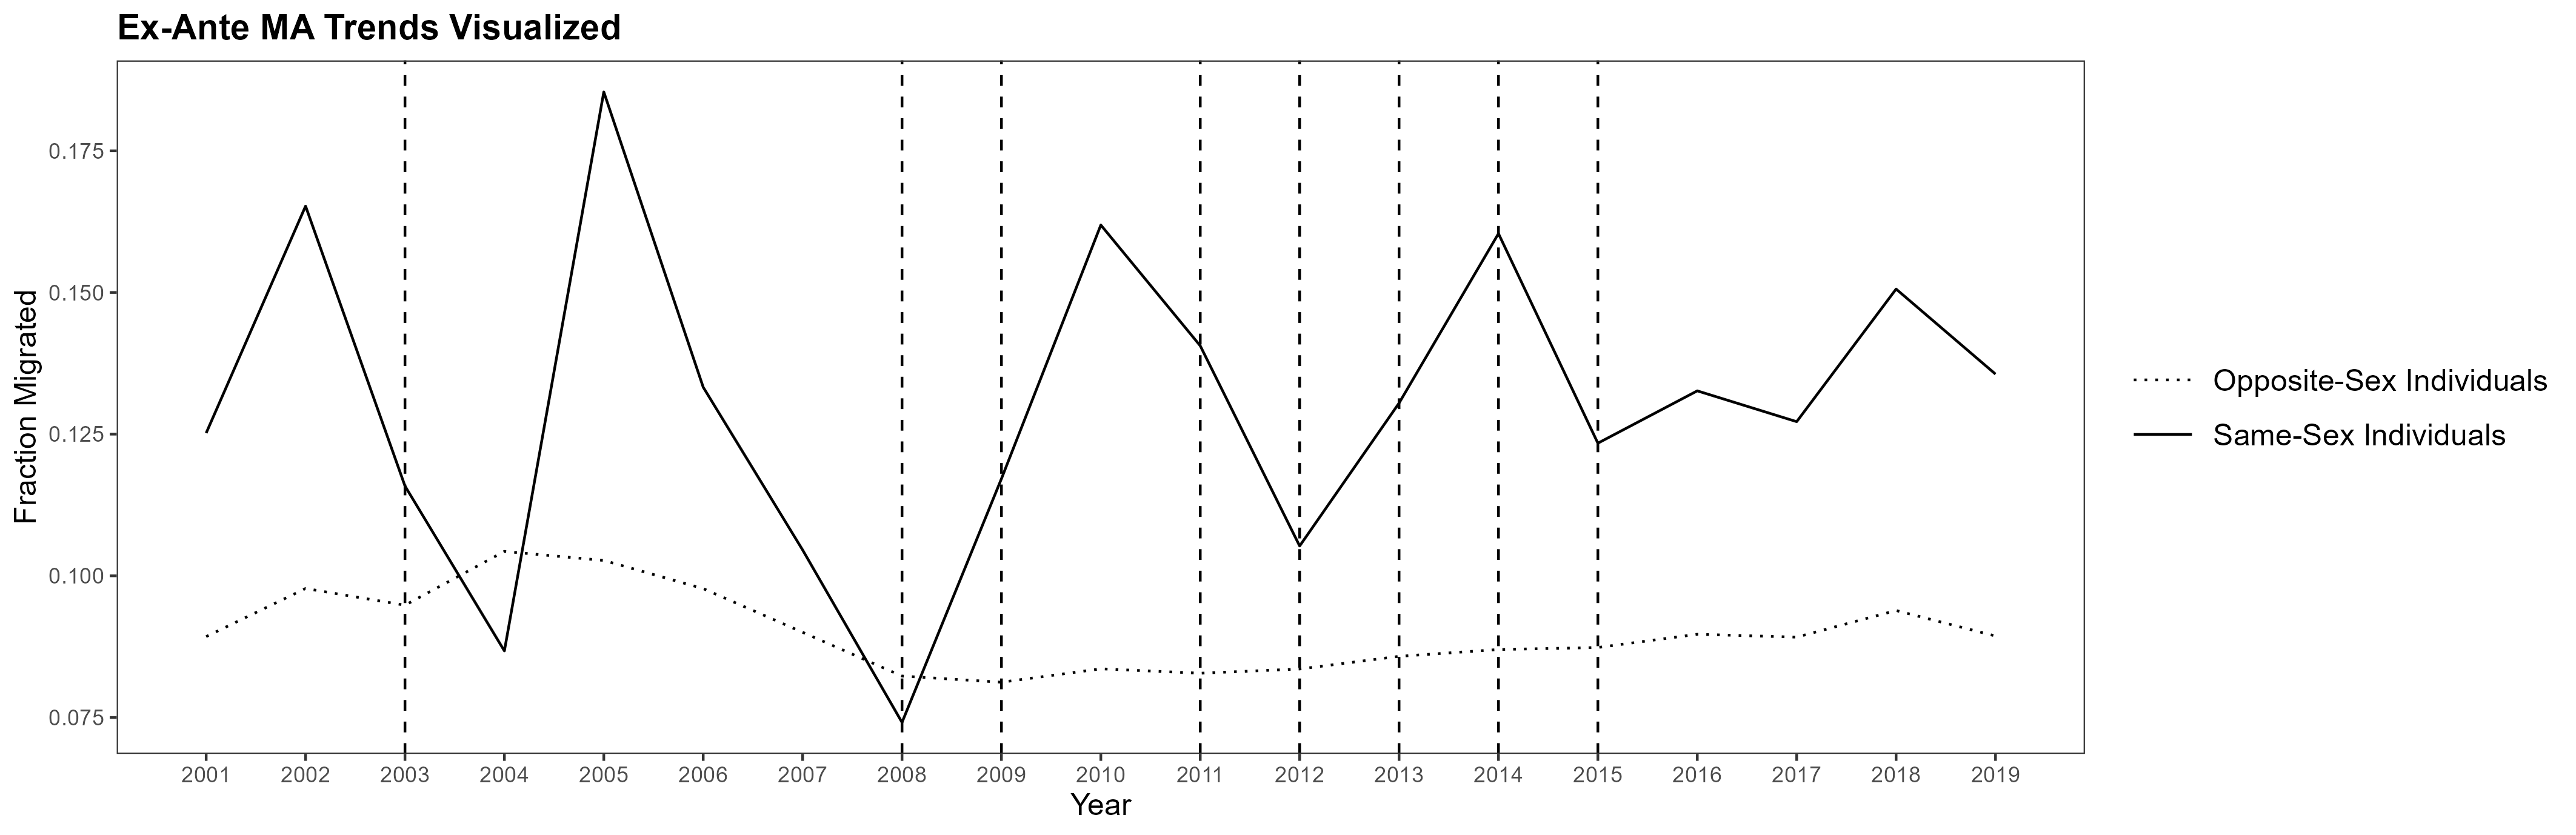
\includegraphics[width=0.75\linewidth, trim= 0 0 0 20, clip]{outputs/summary_stats/MA_ante_trends.png}
%    \caption{MA Push Factor Model}
%    \label{fig: MA_ante_trends}
%    \vspace{0.5em}
%    \begin{minipage}{0.85\textwidth}
%    \small \textit{Note:} There are data reliability concerns between 2005 and 2008 \citep{3, 4, 7}.
%    \end{minipage}
%\end{figure}

\end{document}